\documentclass[twoside,openany,msc]{IUST-Thesis}
\usepackage{amsthm,amssymb,amsmath}
\usepackage[top=40mm, bottom=40mm, left=25mm, right=35mm]{geometry}
\usepackage{graphicx}
\usepackage{framed} 
\usepackage{lastpage}
\usepackage[numbers,square,sort&compress]{natbib}
\usepackage[version=4]{mhchem}
% \usepackage{imakeidx}
\usepackage[xindy]{imakeidx}
\usepackage{pdfpages}

% \usepackage[pagebackref=false,colorlinks=false,linkcolor=black,citecolor=blue]{hyperref}
\usepackage[pagebackref=false]{hyperref}
\hypersetup{
  colorlinks   = true, %Colours links instead of ugly boxes
  urlcolor     = black, %Colour for external hyperlinks
  linkcolor    = black, %Colour of internal links
  citecolor   = black %Colour of citations
}
% \usepackage[xindy,acronym, nonumberlist]{glossaries}
\usepackage[xindy,acronym,nonumberlist=true]{glossaries}
% \usepackage[xindy,,acronym,nonumberlist]{glossaries-extra}

\usepackage{fancyhdr}
\usepackage{setspace}
\usepackage{algorithm}
\usepackage{algorithmic}
\usepackage{subfigure}
% \usepackage{graphicx}
\usepackage{caption}
\usepackage[subfigure]{tocloft}
\usepackage[nottoc]{tocbibind}
\usepackage{chemformula}


% % \usepackage{makeidx}
% % \usepackage[xindy]{imakeidx}
% \makeindex[columns=2,options={-s main.ist}] %load layout
% \makeindex
\newglossary[plg]{persian}{pym}{pbl}{واژه نامه}
\newglossary[elg]{english}{eym}{ebl}{واژه نامه انگلیسی }

% \newglossary{persian}{gls}{glo}{واژه‌نامه‌ی فارسی}
% \newglossary[persian]{persian}{ldx}{ldn}{واژه‌نامه‌ی فارسی}
% \newglossary{english}{gls}{glo}{\lr{Glossary}}
% \newglossary{main}{bls}{glo}{Glossary}
% \newglossary[edx]{english}{idx}{ind}{English Glossary}
\makeglossaries
% \loadglsentries{./pages/Persianglossaries.tex} % Import the glossary entries
% \loadglsentries{./pages/englishglossary.tex} % Import the glossary entries
% \newglossaryentry{computer}
% {
%     name=کامپیوتر,
%     description={ابزاری برای پردازش اطلاعات}
% }
% Acronyms
\newglossaryentry{svm}{type=acronym, name={SVM}, description={Support Vector Machine}}
\newglossaryentry{ann}{type=acronym, name={ANN}, description={Artificial Neural Network}}

\newglossaryentry{رایانه}
{
    type=persian,
    name={رایانه},
    description={دستگاهی الکترونیکی است که برای پردازش اطلاعات و انجام محاسبات استفاده می‌شود.}
}

\newglossaryentry{اینترنت}
{
    type=persian,
    name={اینترنت},
    description={شبکه‌ای از رایانه‌ها و دستگاه‌های مخابراتی است که به یکدیگر متصل شده‌اند و امکان ارتباط و تبادل اطلاعات را برای کاربران فراهم می‌کند.}
}
\newglossaryentry{internet}
{
    type=main,
    name={Internet},
    description={شبکه‌ای از رایانه‌ها و دستگاه‌های مخابراتی است که به یکدیگر متصل شده‌اند و امکان ارتباط و تبادل اطلاعات را برای کاربران فراهم می‌کند.}
}
\newglossaryentry{latex}
{
    type=english,
    name={LaTeX},
    description={A document preparation system}
}
\newglossaryentry{glossaries}
{
    type=english,
    name={Glossaries},
    description={A package for creating glossaries}
}


% \newglossarystyle{persian-block}
% {
%   \renewenvironment{theglossary}
%   {\begin{multicols}{2}\setlength{\parindent}{0pt}}
%   {\end{multicols}}
%   \renewcommand*{\glossaryheader}{}
%   \renewcommand*{\glsgroupheading}[1]{\subsection*{\begin{RTL}##1\end{RTL}}}
%   \renewcommand*{\glsgroupskip}{}
%   \renewcommand*{\glossaryentryfield}[5]{\glstarget{##1}{##2} & ##3\glspostdescription\space ##5\\}
% }
\makeindex[columns=2,options={-s indexstyle.ist}] %load layout

\makeindex[options=-L persian -C utf8, intoc=true,title={\Huge\textbf{فهرست الفبایی}}]
%%%%%%%%%%%%%%%%%%%%%%%%%%
% فراخوانی بسته زی‌پرشین و تعریف قلم فارسی و انگلیسی
\usepackage{xepersian}
\settextfont{XB Niloofar}
% \settextfont{B Nazanin}
% \setmainfont[Ligatures=TeX, Path=./fonts/, Scale=1.2]{XB Niloofar.ttf}
% \settextfont[Scale=1.2, Path=fonts/, BoldFont=B Nazanin Bold.ttf]{B Nazanin.ttf}
\setlatintextfont[Scale=0.8, Path=fonts/, BoldFont=timesbd.ttf]{times.ttf}

%%%%%%%%%%%%%%%%%%%%%%%%%%
% چنانچه می‌خواهید اعداد در فرمول‌ها، انگلیسی باشد، خط زیر را غیرفعال کنید
\setdigitfont[Scale=0.8, Path=fonts/]{XB Zar.ttf}%{Persian Modern}
%%%%%%%%%%%%%%%%%%%%%%%%%%
% تعریف قلم‌های فارسی و انگلیسی اضافی برای استفاده در بعضی از قسمت‌های متن
\defpersianfont\titlefont[Scale=0.8, Path=fonts/]{XB Titre.ttf}
% \defpersianfont\iranic[Scale=1.1]{XB Zar Oblique}%Italic}%
% \defpersianfont\nastaliq[Scale=1.2]{IranNastaliq}

%%%%%%%%%%%%%%%%%%%%%%%%%%
% دستوری برای حذف کلمه «چکیده»
% \renewcommand{\abstractname}{}
% دستوری برای حذف کلمه «abstract»
%\renewcommand{\latinabstract}{}
% دستوری برای تغییر نام کلمه «اثبات» به «برهان»
\renewcommand\proofname{\textbf{برهان}}
% دستوری برای تغییر نام کلمه «کتاب‌نامه» به «مراجع»
\renewcommand{\bibname}{مراجع}
% دستوری برای تعریف واژه‌نامه انگلیسی به فارسی
\newcommand\persiangloss[2]{#1\dotfill\lr{#2}\\}
% دستوری برای تعریف واژه‌نامه فارسی به انگلیسی 
\newcommand\englishgloss[2]{#2\dotfill\lr{#1}\\}
% تعریف دستور جدید «\پ» برای خلاصه‌نویسی جهت نوشتن عبارت «پروژه/پایان‌نامه/رساله»
\newcommand{\پ}{پروژه/پایان‌نامه/رساله }

%\newcommand\BackSlash{\char`\\}

%%%%%%%%%%%%%%%%%%%%%%%%%%
\SepMark{-}

% تعریف و نحوه ظاهر شدن عنوان قضیه‌ها، تعریف‌ها، مثال‌ها و ...
\theoremstyle{definition}
\newtheorem{definition}{تعریف}[section]
%\theoremstyle{theorem}
\newtheorem{theorem}[definition]{قضیه}
\newtheorem{lemma}[definition]{لم}
\newtheorem{proposition}[definition]{گزاره}
\newtheorem{corollary}[definition]{نتیجه}
\newtheorem{remark}[definition]{ملاحظه}
\theoremstyle{definition}
\newtheorem{example}[definition]{مثال}

%\renewcommand{\theequation}{\thechapter-\arabic{equation}}
%\def\bibname{مراجع}
\numberwithin{algorithm}{chapter}
\def\listalgorithmname{فهرست الگوریتم‌ها}
\def\listfigurename{فهرست تصاویر}
\def\listtablename{فهرست جداول}

%%%%%%%%%%%%%%%%%%%%%%%%%%%%
% دستورهایی برای سفارشی کردن سربرگ صفحات
% \newcommand{\SetHeader}{
% \csname@twosidetrue\endcsname
% \pagestyle{fancy}
% \fancyhf{} 
% \fancyhead[OL,EL]{\thepage}
% \fancyhead[OR]{\small\rightmark}
% \fancyhead[ER]{\small\leftmark}
% \renewcommand{\chaptermark}[1]{%
% \markboth{\thechapter-\ #1}{}}
% }
%%%%%%%%%%%%5
%\def\MATtextbaseline{1.5}
%\renewcommand{\baselinestretch}{\MATtextbaseline}
\doublespacing
%%%%%%%%%%%%%%%%%%%%%%%%%%%%%
% دستوراتی برای اضافه کردن کلمه «فصل» در فهرست مطالب

\newlength\mylenprt
\newlength\mylenchp
\newlength\mylenapp

\renewcommand\cftpartpresnum{\partname~}
\renewcommand\cftchappresnum{\chaptername~}
\renewcommand\cftchapaftersnum{:}

\settowidth\mylenprt{\cftpartfont\cftpartpresnum\cftpartaftersnum}
\settowidth\mylenchp{\cftchapfont\cftchappresnum\cftchapaftersnum}
\settowidth\mylenapp{\cftchapfont\appendixname~\cftchapaftersnum}
\addtolength\mylenprt{\cftpartnumwidth}
\addtolength\mylenchp{\cftchapnumwidth}
\addtolength\mylenapp{\cftchapnumwidth}

\setlength\cftpartnumwidth{\mylenprt}
\setlength\cftchapnumwidth{\mylenchp}	

\makeatletter
{\def\thebibliography#1{\chapter*{\refname\@mkboth
   {\uppercase{\refname}}{\uppercase{\refname}}}\list
   {[\arabic{enumi}]}{\settowidth\labelwidth{[#1]}
   \rightmargin\labelwidth
   \advance\rightmargin\labelsep
   \advance\rightmargin\bibindent
   \itemindent -\bibindent
   \listparindent \itemindent
   \parsep \z@
   \usecounter{enumi}}
   \def\newblock{}
   \sloppy
   \sfcode`\.=1000\relax}}
\makeatother

\usepackage{grfext}
\graphicspath{{figures/}}
\usepackage{caption}

\begin{document}
\tracinggroups=1
\pagenumbering{harfi}
% !TeX root=main.tex
% در این فایل، عنوان پایان‌نامه، مشخصات خود، متن تقدیمی‌، ستایش، سپاس‌گزاری و چکیده پایان‌نامه را به فارسی، وارد کنید.
% توجه داشته باشید که جدول حاوی مشخصات پروژه/پایان‌نامه/رساله و همچنین، مشخصات داخل آن، به طور خودکار، درج می‌شود.
%%%%%%%%%%%%%%%%%%%%%%%%%%%%%%%%%%%%
% دانشگاه خود را وارد کنید
\university{علم و صنعت ایران}
% دانشکده، آموزشکده و یا پژوهشکده  خود را وارد کنید
\faculty{دانشکده فیزیک}
% گروه آموزشی خود را وارد کنید
\department{گروه ماده چگال}
% گروه آموزشی خود را وارد کنید
\subject{فیزیک}
% گرایش خود را وارد کنید
\field{ماده چگال}
% عنوان پایان‌نامه را وارد کنید
\title{ترابرد اسپین و بار الکترونی در صفحات دوبعدي بورفین}
% نام استاد(ان) راهنما را وارد کنید
\firstsupervisor{دکتر امیرحسین احمدخان کردبچه}
%\secondsupervisor{استاد راهنمای دوم}
% نام استاد(دان) مشاور را وارد کنید. چنانچه استاد مشاور ندارید، دستور پایین را غیرفعال کنید.
%\firstadvisor{استاد مشاور اول}
%\secondadvisor{استاد مشاور دوم}
% نام دانشجو را وارد کنید
\name{عرفان}
% نام خانوادگی دانشجو را وارد کنید
\surname{نیکان}
% شماره دانشجویی دانشجو را وارد کنید
\studentID{9691117}
% تاریخ پایان‌نامه را وارد کنید
\thesisdate{بهمن  1402}
% به صورت پیش‌فرض برای پایان‌نامه‌های کارشناسی تا دکترا به ترتیب از عبارات «پروژه»، «پایان‌نامه» و »رساله» استفاده می‌شود؛ اگر  نمی‌پسندید هر عنوانی را که مایلید در دستور زیر قرار داده و آنرا از حالت توضیح خارج کنید.
\projectLabel{رساله}

% به صورت پیش‌فرض برای عناوین مقاطع تحصیلی کارشناسی تا دکترا به ترتیب از عبارات «کارشناسی»، «کارشناسی ارشد» و »دکترا» استفاده می‌شود؛ اگر  نمی‌پسندید هر عنوانی را که مایلید در دستور زیر قرار داده و آنرا از حالت توضیح خارج کنید.
\degree{دکتری}

\firstPage
\besmPage
\davaranPage

%\vspace{.5cm}
% در این قسمت اسامی اساتید راهنما، مشاور و داور باید به صورت دستی وارد شوند
%\renewcommand{\arraystretch}{1.2}
\begin{center}
\begin{tabular}{| p{8mm} | p{18mm} | p{.17\textwidth} |p{14mm}|p{.2\textwidth}|c|}
\hline
ردیف	& سمت & نام و نام خانوادگی & مرتبه \newline دانشگاهی &	دانشگاه یا مؤسسه & امضــــــــــــا\\
\hline
۱  & استاد راهنما & دکتر \newline امیرحسین احمدخان کردبچه
& دانشیار & دانشگاه \newline علم و صنعت ایران &  \\
\hline
۲ & استاد داور \newline داخلی	 & دکتر \newline ادریس فیض
آبادي  & استاد & 
دانشگاه  \newline علم ‌و صنعت ایران & \\
\hline
3 & استاد داور \newline داخلی	 & دکتر \newline افشین نمیرانیان  & دانشیار & 
دانشگاه  \newline علم ‌و صنعت ایران & \\
\hline
4 &	استاد داور \newline  خارجی  & دکتر 
\newline علی اصغر شکري
& استاد & دانشگاه \newline  پیام نور تهران  & \\
\hline
5 &	استاد داور \newline  خارجی  & دکتر 
\newline  مهران باقري 
& استادیار & دانشگاه \newline  شهید بهشتی  & \\
\hline
\end{tabular}
\end{center}

\esalatPage
\mojavezPage

 \newpage
\thispagestyle{empty}
{\Large تقدیم به:}\\
\begin{flushleft}
{\huge
%\lr{Pein}\\
%\vspace{7mm}
%و \\
%\vspace{7mm}
\textbf{
پدر و مادرم.
}}
\end{flushleft}

% 
% % سپاس‌گزاری
% \begin{acknowledgementpage}
% سپاس خداوندگار حکیم را که با لطف بی‌کران خود، آدمی را زیور عقل آراست.
% 
% 
% در آغاز وظیفه‌  خود  می‌دانم از زحمات بی‌دریغ استاد  راهنمای خود،  جناب آقای دکتر ...، صمیمانه تشکر و  قدردانی کنم  که قطعاً بدون راهنمایی‌های ارزنده‌  ایشان، این مجموعه  به انجام  نمی‌رسید.
% 
% از جناب  آقای  دکتر ...   که زحمت  مطالعه و مشاوره‌  این رساله را تقبل  فرمودند و در آماده سازی  این رساله، به نحو احسن اینجانب را مورد راهنمایی قرار دادند، کمال امتنان را دارم.
% 
% همچنین لازم می‌دانم از پدید آورندگان بسته زی‌پرشین، مخصوصاً جناب آقای  وفا خلیقی، که این پایان‌نامه با استفاده از این بسته، آماده شده است و همه دوستانمان در گروه پارسی‌لاتک کمال قدردانی را داشته باشم.
% 
%  در پایان، بوسه می‌زنم بر دستان خداوندگاران مهر و مهربانی، پدر و مادر عزیزم و بعد از خدا، ستایش می‌کنم وجود مقدس‌شان را و تشکر می‌کنم از خانواده عزیزم به پاس عاطفه سرشار و گرمای امیدبخش وجودشان، که بهترین پشتیبان من بودند.
% % با استفاده از دستور زیر، امضای شما، به طور خودکار، درج می‌شود.
% \signature 
% \end{acknowledgementpage}
%%%%%%%%%%%%%%%%%%%%%%%%%%%%%%%%%%%%
% کلمات کلیدی پایان‌نامه را وارد کنید
\keywords{یافتن اجتماعات، شبکه‌های پیچیده، الگوریتم‌های گراف}
%چکیده پایان‌نامه را وارد کنید، برای ایجاد پاراگراف جدید از \\ استفاده کنید. اگر خط خالی دشته باشید، خطا خواهید گرفت.
\fa-abstract{
ساختار اجتماع خصوصیتی فراگیر در شبکه‌های پیچیده است. مساله‌ی یافتن اجتماعات در این شبکه‌ها جزو‌ مسایل مورد توجه محققین در
چند سال اخیر بوده است.
اجتماع مجموعه‌ای از گره‌های گراف می‌باشد
که در عین حالی که با هم دارای اتصالات زیادی می‌باشند از بقیه گراف به خوبی مجزا هستند.
گراف‌ ‌شبکه‌های پیچیده دارای خواص ساختاری مانند کوتاهی فاصله‌ دو گره‌ دلخواه هستند
که آن‌ها را از گراف‌های تصادفی مطالعه شده در گذشته متمایز می‌نماید.
از طرفی الگوریتم‌های یافتن اجتماعات را می‌توان به دو دسته‌ی الگوریتم‌های محلی و سراسری تقسیم کرد.
یکی از چالش‌های الگوریتم‌های محلی انتخاب گره‌های دانه است.
در این پایان‌نامه روشی برای یافتن اجتماعات روی گراف شبکه‌های
پیچیده به کمک انتخاب دانه‌های مرغوب و بسط این گره‌ها توسط یک الگوریتم محلی ارایه شده است.
 روش‌ پیشنهادی ۳ مرحله دارد،
 در مرحله‌ی نخست گره‌های گراف ورودی به کمک یک استراتژی حریصانه به چندین افراز تقسیم می‌شوند.
 این افراز‌ها نشان دهنده‌ی اجتماعات اولیه گراف‌ ورودی خواهند بود.
 در گام دوم درون هر زیرگراف حاصل از گره‌های درون یک افراز و اتصالات میان گره‌های آن
 ‌  به دنبال گره‌هایی که به احتمال زیادی به خوبی در بطن یک اجتماع واقع شده‌اند می‌گردیم.
  در این مرحله در هر زیرگراف به صورت موازی به کمک بررسی همسایگی گره‌های
  با درجه‌ بالا، گره‌هایی را که می‌توانند به خوبی نشانگر اجتماع خود باشند را به عنوان گره‌ دانه برمی‌گزینیم.
 در گام آخر اجتماعاتی که هر گره دانه در آن قرار گرفته است را به کمک الگوریتمی که بر پایه محاسبه‌ی
 بردار
 \lr{Personalized Pagerank}
عمل می‌کند، می‌یابیم.
 برای آزمایش کیفیت اجتماعات خروجی
 روش پیشنهادی خود، از ۲۲ گراف استاندارد که در ۷ دسته مختلف از شبکه‌های پیچیده قرار می‌گیرند استفاده نموده ایم.
 برای سنجش کیفیت اجتماعات روش‌ پیشنهادی میزان ۵ معیار مختلف سنجش اجتماعات برای خروجی روش ‌ما و ۳ روش دیگر آزمایش شده است.
 کیفیت اجتماعات روش پیشنهادی برای ۲ معیار از ۵ معیار بسیار بهتر از خروجی دیگر روش‌هاست، برای ۳ معیار دیگر هم عملکرد
 روش‌ پیشنهادی بسیار شبیه عملکرد روش با بهترین خروجی بوده است.
نتایج‌ نشان‌ می‌دهد که نباید تنها درجه‌ یک گره‌ را به عنوان معیار صرف دانه بودن آن انتخاب کرد.
}

\abstractPage

\newpage\clearpage
\tableofcontents
\newpage
\listoffigures \newpage
\listoftables \newpage
% \addcontentsline{toc}{chapter}{\listalgorithmname}
\listofalgorithms \newpage
% \chapter*{فهرست علایم اختصاری}
\addcontentsline{toc}{chapter}{فهرست علایم اختصاری}

\persiangloss{اجتماع}{$C$}
\persiangloss{رسانش}{$\Phi$}
\persiangloss{ماژولاریتی}{$\Omega$}
\persiangloss{گراف}{$G$}
\persiangloss{مجموعه گره‌های گراف $G$}{$V$}
\persiangloss{مجموعه اتصالات گراف $G$}{$E$}
\persiangloss{تعداد گره‌ها}{$n = |V|$}
\persiangloss{تعداد یال‌ها}{$m = |E|$}
\persiangloss{درجه گره $v$}{$deg(v)$}
\persiangloss{تعداد گره‌هایی که $x$ یال دارند}{$N_{deg(x)}$}
\persiangloss{میانگین تعداد یال‌های هر گره گراف $G$}{$a_G$}
\persiangloss{\lr{Clustering Coefficient}}{$CC$}
\persiangloss{قطر حقیقی گراف}{$Dia$}
\persiangloss{قطر موثر گراف}{$Dia_{ef}$}
\persiangloss{مجموعه گره‌های گراف $g$}{$V_{g}$}
\persiangloss{مجموعه اتصالات گراف $g$}{$E_{g}$}
\pagestyle{fancy}

\chapter{فصل مقدمه} 
\pagenumbering{arabic}
\newpage
گرافن اولین ماده دوبعدی کشف شده است [1]. کشف خصوصیات حیرت انگیز گرافن مجموعه ای از مواد جدید را به وجود آورده است که به عنوان "مواد دو بعدی" شناخته می شوند [2-4]. فرم های دو بعدی برای بسیاری از کاربردها یک منطقه نسبتاً هیجان انگیز و جدید است [5 ، 6]. معمولاً مواد دو بعدی دارای بسیاری از خصوصیات فیزیکی برجسته هستند که برای دستگاه های الکترونیکی ، مهندسی نانو ، تبدیل انرژی و فوتونیک امیدوار کننده است [7–11]. با توسعه سریع گرافن ، اخیراً مواد دو بعدی ، مانند فسفرن ، 
\lr{BN} ، ژرمن ، آنتیمونن ، سیلیسن ، آرسنن و دی الكوژنیدهای فلزات انتقالی ، مورد توجه گسترده قرار گرفته اند.

توده ای از مواد با ضخامت اتم از نظر تئوری پیش بینی یا سنتز شده است [12–16]. با کمال تعجب ، آنها ساختارهای متفاوتی از گرافن دارند ، این اختلاف از درجه های متفاوت خمیدگی حاصل می‌شود [17]. علاوه بر مواد دو بعدی لایه برداری شده از نمونه های بالک، برخی از مواد دوبعدی نیز می توانند از مواد بالک بدون فرم لایه ای تولید شوند ، مانند ترکیب بور تخت دوبعدی  \lr{GaN 2D} و هافنن [18 ، 19].

تحقیقات در مورد بور در ترکیبات مختلف را می توان به چند صد سال پیش بازگرداند ، زیرا بور دارای خاصیت فوق العاده ای است که می تواند تقریباً با تمام عناصر دیگر ترکیب شود.


در میان آنها ، نیترید بور شش ضلعی \lr{(h-BN)} یک ترکیب بند وسیع \lr{III-V} است. این یک ماده لایه ای با ساختار گرافیت مانند است که در آن شبکه های مسطح شش ضلعی \lr{h-BN} مرتباً روی هم انباشته می شوند. \lr{h-BN} دارای پایداری شیمیایی بالا ، خصوصیات فیزیکی عالی و هدایت حرارتی بالایی است [20–23].

در سال 2015 ، ورق بور \lr{2D} با موفقیت بر روی بسترهای نقره  \lr{(Ag)} ساخته شد [25]. مطالعه بوروفن محققان زیادی را در بسیاری از زمینه ها مانند علوم مواد ، فناوری نانو ، فیزیک ، شیمی و مواد تغلیظ شده جذب کرده است [13 ، 26 ، 27]. \lr{"Borophene"} نانو صفحه جدید بور با ضخامت اتم برای سنتز در مقیاس بزرگ است [28]. این سبک ترین ماده دوبعدی تا به امروز است. بوروفن همسایه گرافن است و بنابراین ، داشتن برخی از خصوصیات مشابه گرافن مطلوب است [29].

هر دو الکترون $\sigma$ و $\pi$ در بوروفن حالات الکترونیکی سطح فرمی را اشغال می کنند و آن را ابررسانا می کنند. فشار زیاد و فشار خارجی وجود ندارد. بوروفن می تواند بالاترین \lr{Tc} را در بین مواد \lr{2D} داشته باشد. برای ساختارهای بور\lr{2D} ، پیچیدگی شیمیایی و ساختاری ، خصوصیات الکترونیکی و پایداری به طور گسترده مورد بررسی قرار گرفته است [27 ، 30 ، 31].

اخیراً ، یک نانوساختار کاملاً فلزی مبتنی بر بور بر روی یک کریستال نقره با رسوب بخار فیزیکی ، به نام بوروفن، ساخته شده است [32–36]. فازهای زیادی از آلوتروپهای بور بالک و دوبعدی مانند $\alpha$ ، $\beta$ و غیره وجود دارد که از لحاظ نظری پیشنهاد شده اند [37–39]. 

اگرچه ، بور از مشارکت در تشکیل پیوندهای شیمیایی برای ایجاد یک شبکه لانه زنبوری پایدار جلوگیری می کند ، اما ممکن است یک ساختار مسطح پایدار توسط مخلوطی از لانه زنبوری همراه با واحدهای مثلثی ایجاد شود [42،43] این ساختار شامل دو اتم در سلول واحد اولیه است که \lr{2B:Pmmn} نامیده می شود، که در آن \lr{Pmmn} مخفف گروه فضایی 59 است که در یک سیستم بلوری \lr{orthorhombic} وجود دارد. \lr{Xu} و همکاران [44] یک ماده جدید دیراک را پیش بینی کرد: بوروفن هیدروژنه (بوروفان) ، مشخصه‌های دیراک را با سرعت قابل توجه فرمی نشان می دهد که تقریبا دو برابر گرافن است.

ب )  اصول و فرضيات :
یک مخروط دیراک در ساختار نواری بوروفن هیدروژنه (بوروفان) بین نقاط گاما و ایکس دیده می‌شود، در مرجع[41].با مقایسه معادله دیراک برای ذرات با اسپین نیمه صحیح و هامیلتونی موثر بی جرم دو نوار انرژی صفحه که در انرژی های پایین معتبر است. همیلتونین مربوط به مخروط دیراک واقع در $k_d = (0.64،0،0 ±)^{-1}$\AA با معادله زیر آورده شده است:
$$
H_D = v_x \sigma_x p_x + v_y \sigma_y p_y + v_t I p_x
$$

جایی که $\sigma_x$ و $\sigma_y$ ماتریس های پاؤلی هستند و $I$ ماتریس یکانی به بعد 2 است. این عبارت یک مخروط دیراک \lr{2D} ناهمسانگرد کلی را تعریف می کند ، که با سه ثابت $v_x$ ، $v_y$ , $v_t$ توصیف می شود ، که به معنای سرعت در $x$ و $y$ است جهت و درجه شیب به ترتیب. قطری‌سازی این نتایج همیلتونین در پراکندگی انرژی است
$$
\epsilon(k_x,k_y) = (k_x - k_y) \pm \sqrt{(kx_ -k_y)^2 v_x^2 + k_y^2 v_y^2}
$$

طوری که $v_x = 19.58\times 10^5$ \lr{m / s} ، $v_y = 6.32\times 10^5$ \lr{m / s} ، $v_t = -5.06\times 10^5$ \lr{m / s}. یک نمودار کانتور از مخروط ناهمسانگرد دیراک در شکل 4 نشان داده شده است. سرعت در جهات $x$ مثبت و منفی به ترتیب توسط $v_x + | v_t | = 24.64 \times 10^5$  \lr{m / s} و $v_x - | v_t | = 14.52 \times 10^5$ متر در ثانیه $v_x + | v_t | ، v_x - | c_t|$ ، و $v_y$ برابر با $2.95$ ،$ 1.74$ و $0.76$ برابر سرعت فرمی گرافن هستند ($v_f =8.36\times 10^5$ \lr{m/s} ).[41]

روش ماتریس انتقال مورد بررسی قرار گرفته است [45] در این تحقیق تلاش خواهیم کرد که نتایج استفاده از روش تابع گرین غیر تعادلی که در بخش پایانی به آن اشاره شده است را برای این سیستم بررسی نماییم. می توانیم با استفاده از مدل تنگ بست با اضافه کردن اثرات مختلف به همیلتونی از طریق الگوریتم محاسباتی لوپز-سانشو اثر آن را روی ترابرد بررسی نماییم.
\index{مثال}
\chapter{مروری بر ادبیات و کار‌های انجام شده}
\clearpage
\begin{figure*}[!ht]
    \centering
    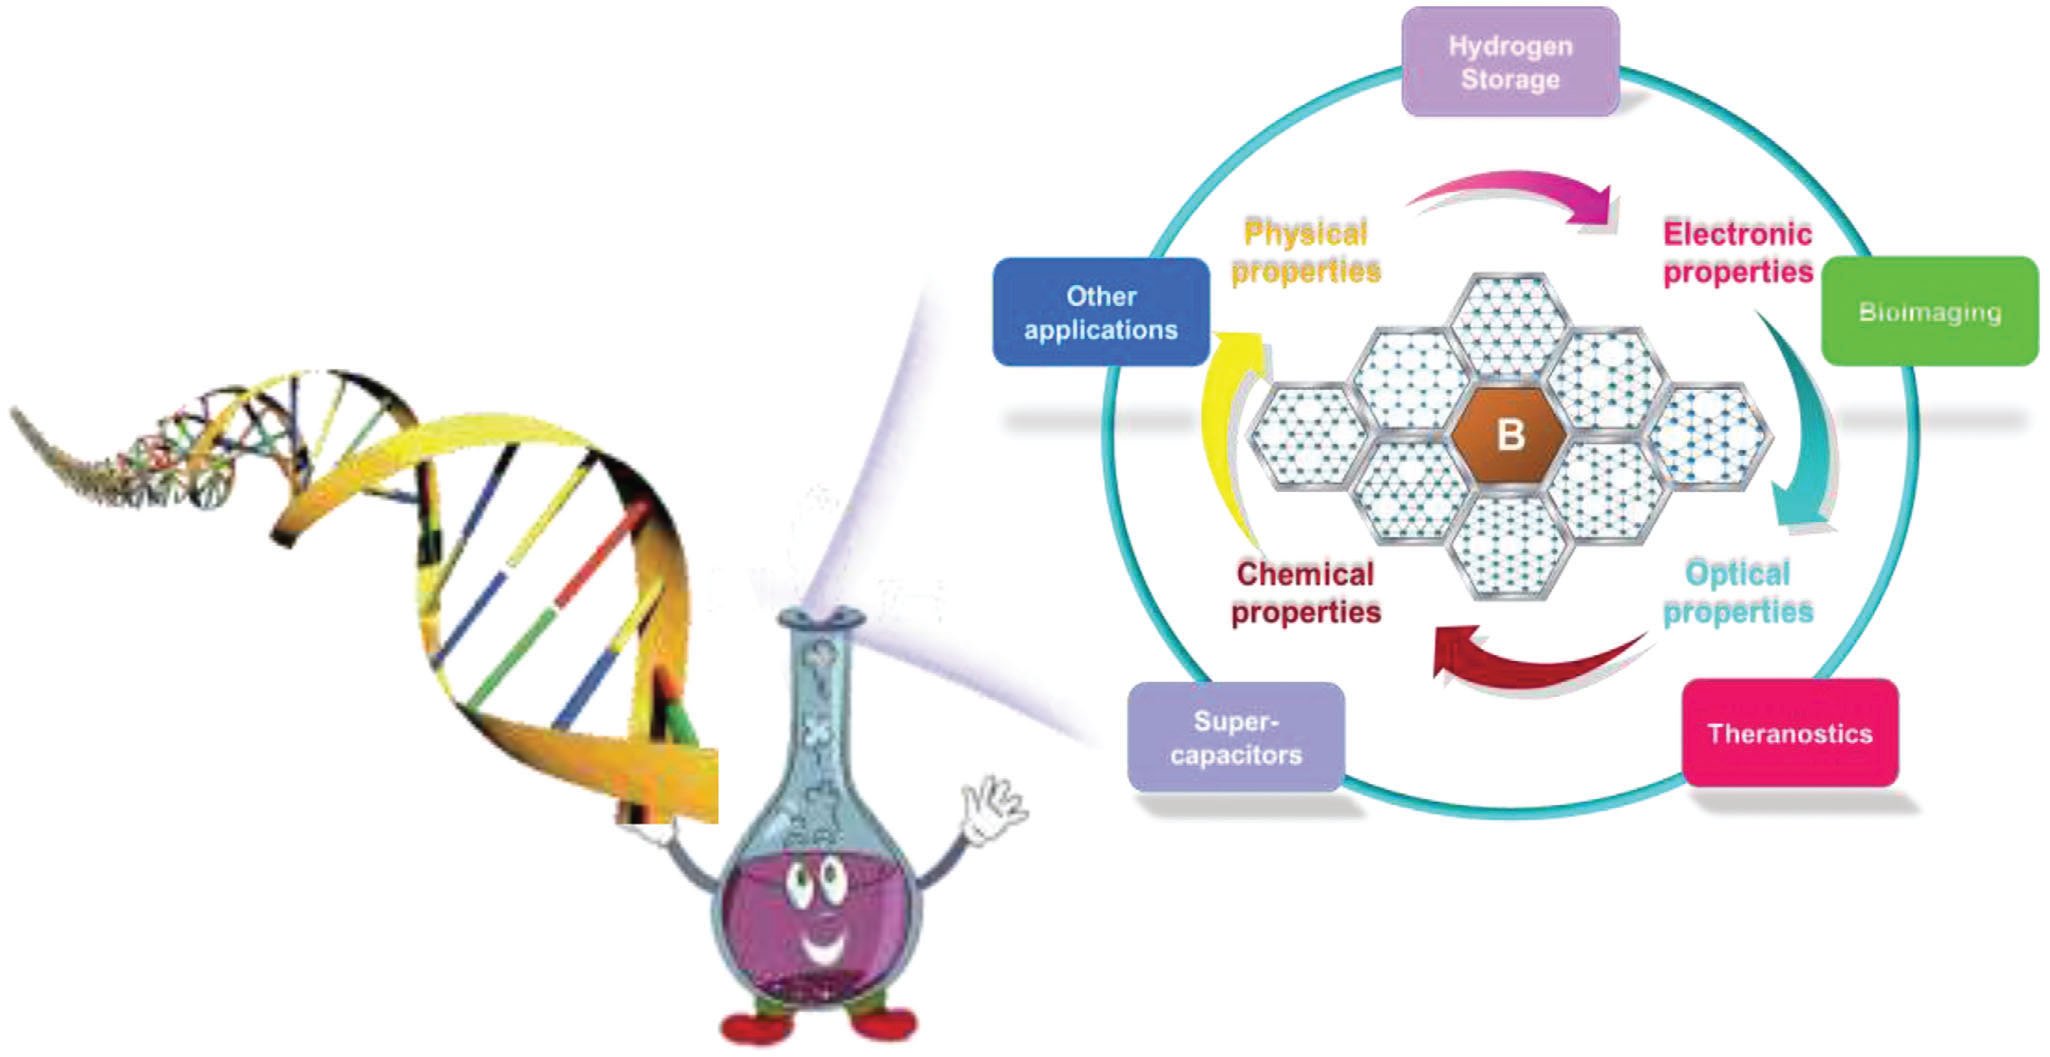
\includegraphics[width=\linewidth]{borophenedev.png}
    \caption{تصویری از توسعه منحصر به فرد بوروفین. نظریه های بوروفین فراوان است. اطلاعات کلیدی موثر بر خواص و سنتز بوروفین از طریق پیش‌بینی نظری، مشابه سنتز پروتئین مبتنی بر ژن، به دست آمده است تا به طور کلی سنتز بوروفین را هدایت کند.}
    \label{fig:borophenedev}
\end{figure*}
\section{مقدمه:}
نانومواد دو بعدی به دلیل ویژگی های منحصر به فرد و فوق العاده شان توجه زیادی را از جامعه علمی به خود جلب کرده اند.\cite{huangGraphenebasedComposites2012, huangGrapheneBasedMaterialsSynthesis2011}بر خلاف مواد \gls{bulk}، صفحه‌های نانوی فوق نازک دو بعدی که اکثر اتم‌های‌شان در معرض سطح قرار دارند، دارای سطح ویژه بزرگتر، فعالیت شیمیایی و فیزیکی بالاتر و اثرات \gls{quantum confinement} هستند که به آنها ویژگی های خاص فوتونی، الکترونی، کاتالیزوری و مغناطیسی می‌بخشد و پتانسیل کاربردی بالایی در مواد زیست سازگار، \gls{drug carriers}، بیوسنسورها، وسایل الکترونی و غیره دارند.\cite{lu2DTransitionMetalDichalcogenideNanosheetBasedComposites2016, chhowallaChemistryTwodimensionalLayered2013, sunElectronicStructuresSiC2008} در سال 2004 ظهور گرافین باعث تحول بزرگی در حوزه مواد شد و کاربردهای مواد دو بعدی را در زمینه های مختلف به طور چشمگیری بهبود بخشید. \cite{novoselovElectricFieldEffect2004, geimRiseGraphene2007} با این حال، \gls{bandgap} صفر گرافین بسیاری از کاربردهای آن را در قطعات الکترونیکی، تصویربرداری زیستی و فتودینامیک تراپی محدود می‌کند. در سال های اخیر، محققان به دنبال یافتن مواد دو بعدی با ساختار لانه زنبوری مانند گرافین یا صفحه های نانوی دو بعدی تک عنصری هستند که در گروه همانند یا مجاور عنصر کربن قرار دارند، به امید توسعه مواد مشابه گرافین با خواص عالی. خوشبختانه ظهور مواد دارای ساختار مشابه گرافین مانند سولفیدهای فلزات واسطه \gls{TMD}\cite{dingDefectEngineeredBioactive2019, liRatiometricImmunoassaysBuilt2019}، نیترید بور مربعی \gls{h-BN}\cite{deanBoronNitrideSubstrates2010}،و نیترید بور گرافیتی \gls{g-C3N4}\cite{caoPolymericPhotocatalystsBased2015}و همچنین مواد دو بعدی تک عنصری مانند \gls{Borophene}\cite{fengExperimentalRealizationTwodimensional2016}،سیلسین\cite{fengEvidenceSiliceneHoneycomb2012,chenEvidenceDiracFermions2012,duTuningBandGap2014}، استانن\cite{gouStraininducedBandEngineering2017, zhuEpitaxialGrowthTwodimensional2015}،و ژرمانن \cite{niTunableBandgapSilicene2012} نه تنها می توانند کمبود \gls{bandgap} صفر گرافین را جبران کنند، بلکه دارای خواص ویژه دیگری نیز هستند که انتظار می‌رود عملکردها و کاربردهای جدیدی را به ارمغان بیاورند. در مقایسه با سایر مواد دو بعدی، نانوموادهای تک عنصری دارای سه مزیت منحصر به فرد هستند: 1) سازگاری بیشتر با فناوری نیمه هادی موجود. به عنوان مثال، عناصر سیلیسیم و ژرمانیم عناصر اصلی ساخت مواد نیمه هادی سنتی هستند. 2) به دلیل تشکیل شده از یک عنصر، سنتز با کیفیت بالا نسبتا ساده است. 3) تجزیه و \gls{metabolize} شدن توسط سیستم های بیولوژیکی آسان تر است. فسفر سیاه یکی از نانوموادهای دو بعدی تک عنصری با سازگاری زیستی خوب است. این ماده می تواند در بدن به فسفات تجزیه شود و در حفظ بسیاری از فعالیت‌های فیزیولوژیکی مهم به عنوان ماده اولیه برای \gls{ATP} و \gls{DNA} شرکت کند.\cite{shaoBiodegradableBlackPhosphorusbased2016,taoBlackPhosphorusNanosheets2017}علاوه بر این، سطح ویژه بسیار بالا و سطوح مختلف پاسخ به \gls{pH}، نور، الکتریسیته و غیره، باعث می شود نانوموادهای دو بعدی تک عنصری به گزینه های برتر برای وسایل الکترونی، انتقال دارو، درمان نوری، تصویربرداری زیستی و سایر زمینه‌ها تبدیل شوند. \cite{liEngineeredFunctionalized2D2020,shiPHSensitiveNanoscaleMaterials2020}

همانطور که \gls{Borophene} یکی از مواد نانوی تک عنصری دوبعدی به حساب می‌آید، شباهت زیادی به گرافین و فسفر سیاه دارد. نه تنها سطح ویژه‌ای بالا و ظرفیت بارگذاری دارو بالایی دارد (\gls{Borophene}: 114\% \cite{jiNovelTopDownSynthesis2018}، فسفر سیاه: 108\% \cite{taoBlackPhosphorusNanosheets2017}، گرافین اکسید: 200\% \cite{zhangFunctionalGrapheneOxide2010}، سایر نانومواد: \lr{10-30\%}، بلکه در شرایط اسیدی، نوری و گرمایی قادر به رهاسازی دارو به صورت هوشمندانه نیز هست. \gls{Borophene} یکی از مرموزترین نانوموادهای تک عنصری دوبعدی است که منحصر به فردترین ویژگی‌اش \gls{Polymorphism} بودن (چند ساختار متفاوت داشتن) آن است. \gls{Borophene}‌هایی که با روش‌های مختلف و تحت شرایط گوناگون ساخته می‌شوند، ساختارهای متفاوتی دارند و این \gls{Allotropes} ویژگی‌های گوناگونی هم از خود نشان می‌دهند. برای مثال، پیش‌بینی می‌شود \gls{Borophene} فاز \lr{Pmmn} با مخروط‌های دیراک و ویژگی‌های الکتریکی جدید،\gls{intriguing Dirac materials} باشد \cite{zhouSemimetallicTwoDimensionalBoron2014}. خواص فاز $\beta_{12}$ \gls{Borophene} و فاز $\alpha$ \gls{Borophene} هم تفاوت دارند؛ اولی ناهمسانگرد و دومی همسانگرد است \cite{zhouSuperiorLatticeThermal2017, xiaoLatticeThermalConductivity2017}. این به این معنی است که می‌توانیم با کنترل و تنظیم شرایط ساخت، \gls{Borophene}‌هایی را سنتز کنیم که نیازهای کاربردی ما را برآورده کنند. امروزه هنوز گزارش‌های کمی در مورد \gls{Borophene} وجود دارد و این ویژگی‌های شگفت‌انگیز مشاهده شده، تنها بخش کوچکی از این کوه یخی هستند؛ هنوز جزئیات بسیاری برای کشف توسط محققان باقی مانده است.

بور، تنها عنصر نیمه‌رسانا در گروه \lr{IIIA} و پنجمین عنصر در جدول تناوبی عناصر، هم‌جوار کربن و دارای اوربیتال‌های ظرفیتی مشابه آن است. \cite{forteInitioPredictionBoron2010}این شباهت‌ها نشان می‌دهد که \gls{Borophene}، فلز دوبعدی سبک، ممکن است ویژگی‌های جالب مشابه گرافین داشته باشد. \cite{huangTwoDimensionalBoronPolymorphs2017, liuIntermixingPeriodicSelfassembly2018} ساختار الکترونی خاص، مکانیزم پیوند پیچیده و هم‌بستگی نزدیک با عناصر کربن نشان می‌دهد که \gls{Borophene} احتمالا خواص عالی مشابه گرافین خواهد داشت و حتی می‌تواند از آن فراتر رفته و به ابرماده جدیدی تبدیل شود. در واقع، محاسبات نظری حاکی از آن است که \gls{Borophene} دارای ساختارهای \gls{Allotropes} کم‌بعدی زیاد و خواص جالبی است. \cite{liuBorophenegrapheneHeterostructures2019} \gls{Boustani} و همکاران \cite{boustaniSYSTEMATICLSDINVESTIGATION1994} پیش‌بینی کردند که خوشه‌های بور ممکن است ساختاری شبه صفحه‌ای\LTRfootnote{quasi-planar} تشکیل دهند که نشان می‌دهد \gls{Borophene} دوبعدی را می‌توان به‌صورت تجربی تهیه کرد.به‌علت مکانیزم‌های پیوند پیچیده و ساختار غیرلایه‌ای بور \gls{bulk}، سنتز تجربی \gls{Borophene} تا سال 2015 به دست نیامد، زمانی که گروه‌های تحقیقاتی \gls{Guisinger} \cite{mannixSynthesisBorophenesAnisotropic2015} و \gls{Wu} \cite{fengExperimentalRealizationTwodimensional2016} به‌طور جداگانه بر روی \lr{Ag(111)} به سنتز آن دست یافتند. برخلاف اکثر مواد سنتی که با آزمایش‌های تجربی مستقیم طراحی می‌شوند، طراحی \gls{Borophene} با نظریه‌هایی آغاز شد که ویژگی‌های بالقوه و روش‌های احتمالی تهیه آن را پیش‌بینی می‌کردند و به‌طور موفقیت‌آمیزی فرآیند تهیه آزمایشگاهی و کاربردهای بعدی \gls{Borophene} را هدایت کردند (طرح‌واره\ref{fig:borophenedev}). توسعه \gls{Borophene} بدون شک نمونه موفقی از پروژه ژنوم مواد (\gls{MGI}) است. همانطور که انسان‌ها ژن‌هایی دارند که ویژگی‌های آن‌ها را تعیین می‌کند، مواد نیز دارای «ژن‌های» کلیدی هستند که خواص آن‌ها را مشخص می‌کنند. \gls{MGI} پیش‌نهاد می‌کند قبل از کشف مواد ناشناخته، رابطه بین ترکیب، ساختار و خواص مواد از طریق تحقیقات نظری روشن شود تا کارایی سنتز مواد، هزینه تحقیقات مواد و موفقیت طراحی مواد افزایش یابد. ظهور و تکامل \gls{Borophene} الگویی برجسته برای سنتز مواد جدید ارائه می‌دهد.
\begin{figure*}
    \centering
    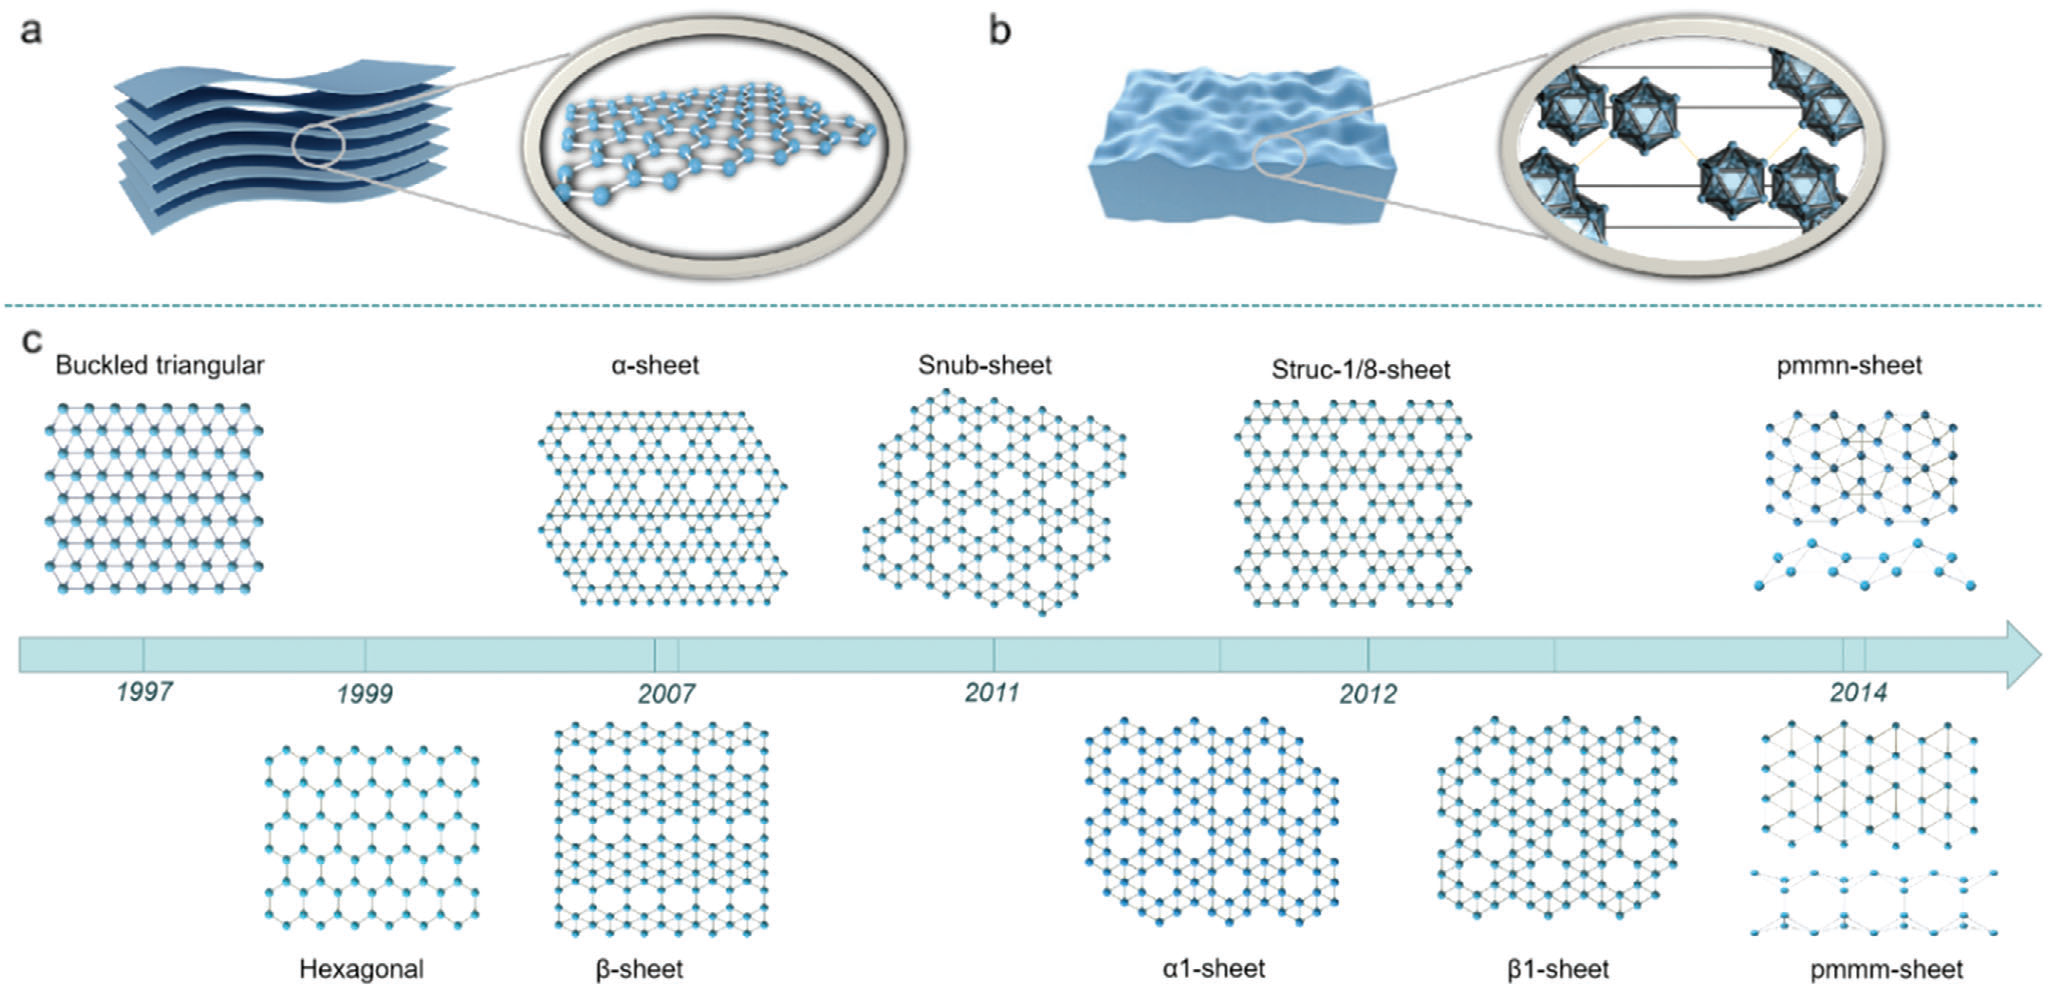
\includegraphics[width=\textwidth]{theory-borophene.png}
    \caption{انواع مختلف پیش سازهای \gls{bulk} مواد دو بعدی. الف) ساختار گرافیت \gls{bulk} که لایه آن توسط نیروی واندروالس به هم متصل شده است. ب) ساختار بور \gls{bulk} که واحدهای ساختاری آن از طریق پیوند پیچیده ترکیب می شوند. ج) تاریخچه توسعه بوروفین در مدل های نظری. ساختار مثلثی کماندار بوروفین برای اولین بار در سال 1997 پیش بینی شد. سپس یک ساختار جدید بور تک لایه، $\alpha$-صفحه، متشکل از شبکه مثلثی و سوراخ های لانه زنبوری شش ضلعی، از طریق محاسبه به دست آمد. اتم‌های بور صفحه $\alpha$ در یک صفحه قرار دارند که انرژی آن کمتر از ساختار مثلثی کمانش‌شده است که در مطالعات قبلی به عنوان پایدارترین ساختار در نظر گرفته می‌شد. بر این اساس، طی سال های 2007-2014، یک سری از ساختارهای کلاسیک بوروفین مانند صفحات $\beta$، \lr{snub}، $\alpha 1$، \lr{struc-1/8}، $\beta 1$، \lr{Pmmn}، \lr{Pmmm} رخ داده است. از طریق آرایش متفاوت شبکه های شش ضلعی و مثلثی. انرژی این سازه‌ها بسیار کم و تقریباً برابر است.}
    \label{theoryborophene}
\end{figure*}
\section{بررسی تئوری ساختار بور دوبعدی}
به دلیل کمبود الکترون در لایه بیرونی، اتم‌های بور به راحتی می‌توانند پیوندهای شیمیایی تشکیل دهند؛ بنابراین، بور از نظر شیمیایی فعال بوده و ترکیباتی با ساختارهای کریستالی متنوع ایجاد می‌کند. ساختار اصلی کریستالی بور توده (شکل \ref{theoryborophene}.ب) \gls{Icosahedron} بر اساس یک \ce{B12} به عنوان واحد ساختاری پایه استوار است، و انواع مختلف کریستال‌های بور از طریق اتصالات و روش‌های پیوند مختلف روی \gls{Icosahedron} \ce{B12} شکل می‌گیرند. \cite{albertBoronElementaryChallenge2009} بنابراین، توده بور برخلاف گرافین (شکل \ref{theoryborophene}.الف) یک ساختار لایه‌ای ندارد که باعث پیچیده و دشوار شدن تهیه \gls{Borophene} می‌شود.

در سال 2006، \gls{Kunstmann} , \gls{Quandt} \cite{kunstmannBroadBoronSheets2006} برای اولین بار ساختار پایه صفحه‌های بور دوبعدی را پیش‌بینی کردند و راز \gls{Borophene} را آشکار ساختند. در سال 2014، \gls{Wang} و همکاران \cite{zhaiObservationAllboronFullerene2014} برای اولین بار نشان دادند که \ce{B36} یک خوشه \gls{Borophene} شبه مسطح بسیار پایدار با ساختار توخالی شش ضلعی است و تأیید کردند که خوشه‌های \gls{Borophene} تک اتمی با حفره‌های شش ضلعی امکان‌پذیر هستند. همچنین برای اولین بار مفهوم \gls{Borophene} را ارائه دادند. در سال‌های اخیر، تحقیقات تئوری \gls{Borophene} به نتایج مثمری رسیده است، اما روش‌های سنتز و کاربردهای بور همچنان اندک هستند.

اولین سنتز \gls{Borophene} در آزمایشگاه در سال 2015 به دست آمد. \gls{Borophene} دارای انواع ساختارها است که بر اساس الگوهای ترکیب طبقه‌بندی می‌شوند: الف) صفحه \gls{distorted hexagonal} \gls{DH}، ب) صفحه \gls{buckled triangular} \gls{BT}، و ج) صفحه مثلثی-شش ضلعی ترکیبی \gls{MTH}، یا بر اساس \gls{coordination number} (\gls{CN}): نوع $\alpha$ (\lr{CN = 5، 6})، نوع $\beta$ (\lr{CN = 4، 5، 6})، نوع $\chi$ (\lr{CN = 4، 5})، نوع $\delta$ (\lr{CN = m}، که \lr{m} یک عدد واحد است)، و نوع $\psi$ (\lr{CN = 3، 4، 5}).\cite{wuTwoDimensionalBoronMonolayer2012}
صفحه \gls{DH} (ساختار شش ضلعی شکل \ref{theoryborophene}.ج)، ساختاری تقریبا مسطح متشکل از شش ضلعی‌های پیچ خورده \cite{bezuglyHighlyConductiveBoron2011}است، مشابه گرافین. صفحه \gls{BT} (ساختار مثلثی خمیده شکل \ref{theoryborophene}.ج)، صفحه‌ای است که واحد پایه آن \ce{B7} است. \ce{B7} یک ساختار هرمی شکل است که با قرارگیری یک اتم بور در وسط یک شش ضلعی اتم‌های بور تشکیل می‌شود. \cite{mannixSynthesisBorophenesAnisotropic2015, wuTwoDimensionalBoronMonolayer2012} اتم بور مرکزی، شش ضلعی را به شش مثلث کوچک تقسیم می‌کند، به طوری که مثلث نیز واحد پایه صفحه \gls{BT} است.

صفحه \gls{MTH} (صفحه $\alpha$ شکل \ref{theoryborophene}.ج) از یک نقش \gls{motif} شش ضلعی توخالی (\gls{HHM}) و یک نقش \gls{motif} مثلثی (\gls{TM}) تشکیل شده است که با تنظیم نسبت آنها منجر به انواع مختلف صفحات \gls{MTH} می‌شود. \cite{yangInitioPredictionStable2008, tianPlanar2hB26H82013, penevPolymorphismTwoDimensionalBoron2012, tangFirstprinciplesStudyBoron2010, lauThermodynamicStabilityNovel2008, lauStabilityElectronicProperties2007} با ترکیب این دو طبقه‌بندی، می‌توانیم متوجه شویم که هم صفحه \gls{DH} و هم صفحه \gls{BT} به صفحه نوع $\delta$ تعلق دارند و صفحه \gls{MTH} شامل تمام صفحات به جز نوع $\delta$ می‌شود.

چندشکلی یکی از مهم‌ترین ویژگی‌های \gls{Borophene} است که به دلیل مکانیزم پیوند پیچیده بین اتم‌های بور و انرژی‌های تشکیل بسیار نزدیک \gls{Borophene} آزاد (بدون تکیه‌گاه) است. در سال 2006، \gls{Kunstmann} و همکاران \cite{kunstmannBroadBoronSheets2006} برای اولین بار ساختار پایه بور دوبعدی را بر اساس اصل \gls{Aufbau} پیش‌بینی کردند و ساختار خمیده با \ce{B7} به عنوان واحد پایه (شکل \ref{fig:charecterboro}.الف) را پیشنهاد دادند، که ساختار اصلی \gls{Borophene} در مطالعات نظری اولیه است. در سال 2007، \gls{Tang} و همکاران \cite{tangSelfdopingBoronSheets2009, tangNovelPrecursorsBoron2007} یکی از کلاسیک‌ ترین ساختارهای غالب انرژی، یعنی صفحه $\alpha$ را پیش‌بینی کردند. اتم‌های بور صفحه $\alpha$ در یک صفحه قرار دارند که انرژی آن به ازای هر اتم 0.12 الکترون ولت کمتر از ساختار مثلثی خمیده است که قبلا پایدارترین در نظر گرفته می‌شد. این را می‌توان به عنوان حذف اتم‌ها از شبکه مثلثی مسطح در نظر گرفت؛ یعنی بر اساس صفحه مثلثی خمیده (\gls{BT})، با حذف اتم بور مرکزی واحد پایه \ce{B7}، می‌توان حفره شش ضلعی توخالی را به دست آورد و در نتیجه ساختار ترکیبی از حفره‌های شش ضلعی و شبکه‌های مثلثی را ایجاد کرد. صفحه $\alpha$ را می‌توان به عنوان گسترش \ce{B80} در نظر گرفت که همه اتم‌های بور در یک صفحه با انرژی کم قرار دارند. تعداد و توزیع شش ضلعی‌های توخالی (\gls{HH}) ساختارهای مختلف \gls{Borophene} را تعیین می‌کند.
\begin{equation}
    \eta=\frac{\text{\lr{No. of hexagon holes}}}{\text{\lr{No. of atoms in the original triangular sheet}}}
\end{equation}

مقدار $\eta$ و الگوی حفره‌های شش ضلعی، انرژی بور دوبعدی را تعیین می‌کنند و سیستم \gls{self-doping} می‌تواند با بهینه کردن $\eta$، \gls{stability} بهینه را حفظ کند. طبق فرمول، $\eta$ صفحه \gls{BT} برابر با 0، صفحه \gls{DH} برابر با 1/3 و صفحه $\alpha$ برابر با 1/9 است. \cite{yuPredictionTwoDimensionalBoron2012} با این حال، از آنجایی که چیدمان‌های متعددی از حفره‌های شش ضلعی در \gls{Borophene} وجود دارد، پیش‌بینی مستقیم همه ساختارهای ممکن با استفاده از روش تئوری تابع چگالی (\gls{DFT}) غیر واقعی است. \gls{Yakobson} و همکاران \cite{penevPolymorphismTwoDimensionalBoron2012} \gls{Borophene} را به عنوان \gls{pseudo-alloy} $B_{1-\nu[]\nu}$ در نظر گرفتند که از حفره‌های شش ضلعی و شبکه‌های مثلثی تشکیل شده است، تا به طور مؤثر تنوع و پایداری ساختاری را ارزیابی کنند. در آنجا، مکان‌های خالی در شبکه‌های مثلثی با بسته‌بندی بسته "[]" نامگذاری شده‌اند و $\nu = m/N$ غلظت حفره‌های شش ضلعی و تعداد حفره‌های شش ضلعی در یک سلول فوقانی با $N$ موقعیت شبکه با $m$ نشان داده می‌شود.\cite{zhangTwodimensionalBoronStructures2017} آن‌ها همچنین با محاسبات نظری به این نتیجه رسیدند که \gls{Borophene} زمانی که غلظت حفره‌های شش ضلعی بین 10\% تا 15\% باشد نسبتاً پایدار است و انرژی‌های پیوستگی \gls{Borophene} با ساختارهای مختلف در محدوده باریکی از غلظت‌های حفره‌های شش ضلعی که به آن اشاره شد، بسیار کم و نزدیک به هم هستند. بر اساس این مطالعات نظری، ساختارهای پایدارتری مانند \lr{g1/8-sheet}،\lr{g2/15-sheet}،\lr{$\alpha_1$-sheet}،\lr{$\beta_1$-sheet}،\lr{snub-sheet}،\lr{struc-1/8-sheet}،\lr{Pmmn} و\lr{2-Pmmm} به ترتیب پیش‌بینی شده‌اند. \cite{zhouSemimetallicTwoDimensionalBoron2014, wuTwoDimensionalBoronMonolayer2012, penevPolymorphismTwoDimensionalBoron2012, yuPredictionTwoDimensionalBoron2012, zopeSnubBoronNanostructures2011} \ref{theoryborophene} ساختارهای خاص آن‌ها را بر اساس سال کشف نشان می‌دهد. \gls{Borophene} به دست آمده به صورت تجربی، اغلب به دلیل مشابه بودن انرژی‌های ساختارهای پایدار به لحاظ ترمودینامیکی، از ساختارهای مختلفی تشکیل شده است.

% \section{سنتز بوروفین}
% \begin{figure*}
%     \centering
%     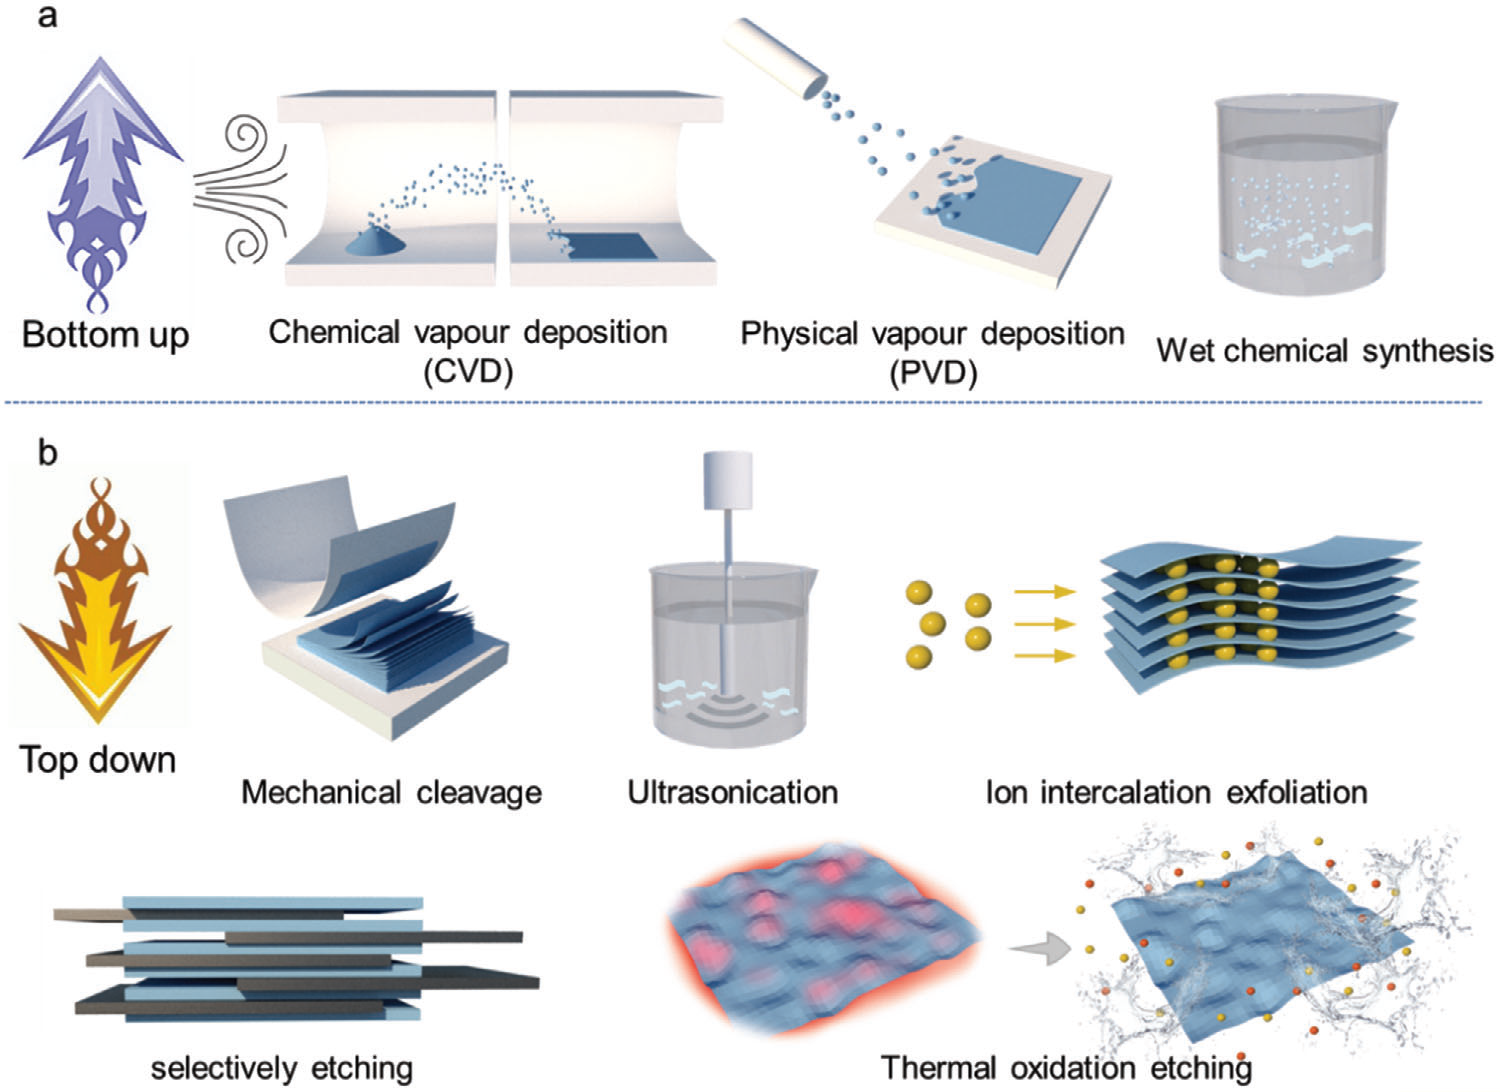
\includegraphics[width=0.7\linewidth]{synthesis.png}
%     \caption{روش سنتز اصلی نانوصفحات دو بعدی الف) روش پایین به بالا: \lr{CVD}، \lr{PVD}، و مواد شیمیایی مرطوب. ب) روش بالا به پایین: برش مکانیکی، فراصوت، لایه برداری بین یونی، اچ کردن انتخابی، و اچ اکسیداسیون گرمایی.}
%     \label{fig:borosynthesis}
% \end{figure*}
% تکنیک‌های «پایین به بالا» و «بالا به پایین» دو روش اصلی برای تهیه نانومواد دو بعدی هستند. رویکرد "پایین به بالا" شامل رسوب فیزیکی بخار \gls{PVD}، \cite{parkCrystallizationInducedPropertiesMorphologyControlled2014, zhaoPatternedGrowthVertically2010, zhaoVerticalOrganicNanowire2009} رسوب بخار شیمیایی \lr{(CVD)}،\cite{zhangReviewChemicalVapor2013, akhavanToxicityGrapheneGraphene2010} و روش های سنتز شیمیایی مرطوب، \cite{hanSynthesisStructuralTransformations2013, wuWelldefinedBiOClColloidal2015} در میان دیگران است (شکل \ref{fig:borosynthesis}.الف\cite{mannixSynthesisChemistryElemental2017}. \gls{CVD} شامل تشکیل یک لایه روی یک بستر از طریق پیش سازهای فاز گاز مربوطه است که روی آن واکنش می دهند. محیط، بسترها و پیش سازها سه عامل بسیار مهم بر خواص و رشد محصولات در این روش هستند. اکسیدهای فلزی، گرافین و \gls{h-BN} همگی توسط \gls{CVD} سنتز شده‌اند. در طول فرآیند \gls{PVD}، منبع ماده از طریق روش فیزیکی در شرایط خلاء به حالت گازی تبخیر می‌شود و روی یک بستر رسوب می‌کند تا یک فیلم کاربردی تشکیل دهد. "
% صفحه های نانو دو بعدی از مواد بدون لایه اغلب توسط واکنش های شیمیایی در محلول تهیه می شوند که سنتز شیمیایی مرطوب نامیده می شود. بسیاری از مواد مانند \lr{\ce{CuS}}، \lr{\ce{Co3O4}}، $\alpha$-\lr{\ce{Fe2O3}}، \lr{\ce{WO3}} و \lr{\ce{Rh}} با این روش پربازده و کم هزینه تهیه شده‌اند. به طور کلی، رویکردهای پایین به بالا را می توان برای سنتز تقریباً همه انواع نانومواد دو بعدی استفاده کرد. 

% رویکردهای "بالا به پایین" شامل \gls{Mechanical cleavage}، \cite{liPreparationApplicationsMechanically2014, yiReviewMechanicalExfoliation2015} \gls{ultrasonication}، \cite{nicolosiLiquidExfoliationLayered2013} \gls{intercalation exfoliation} یونی، \cite{yuwenRapidPreparationSinglelayer2016, zengSingleLayerSemiconductingNanosheets2011} و \gls{etching} \cite{anasoriTwoDimensionalOrderedDouble2015, naguibNewTwoDimensionalNiobium2013, naguibTwoDimensionalNanocrystalsProduced2011} (شکل \lr{2b}) است. \gls{Mechanical cleavage} به نیروهای \gls{shear} برای غلبه بر نیروهای واندروالس بین لایه‌های اتصال متکی است و به طور گسترده در لایه‌برداری مواد دو بعدی از مواد \gls{bulk} استفاده می‌شود.
% فراصوت بسته به نیروهای \gls{shear} باعث لایه برداری مایع می شود. انرژی صوتی آن می تواند مواد لایه ای مانند گرافیت و \ce{MoS2} را جدا کند. در این روش می توان اندازه، کیفیت و پراکندگی مواد دو بعدی را با حلال فراصوت و زمان کنترل کرد. مزایای استفاده از اولتراسونیک هزینه کم و مقیاس تولید بزرگ است، اما بازده مواد دو بعدی تک لایه کم است. در طول لایه برداری یونی، یون‌ها در فاصله لایه‌ها قرار می‌گیرند تا نیروهای واندروالس بین لایه‌ها را کاهش دهند و باعث ایجاد لایه برداری شوند. مواد لایه ای، از جمله دی‌کالکوژنیدهای فلزات واسطه \ch{(TMDs)} و گرافیت، می توانند به راحتی با این روش لایه برداری شوند. روش‌های بالا به پایین ذکر شده در بالا عمدتاً برای جامدات واندروالسی مناسب هستند، در حالی که روش‌های اچ مانند اچ اسید و اچ اکسیداسیون گرمایی معمولاً در جامدات غیر واندروالسی استفاده می‌شوند. اچینگ و لایه برداری انتخابی برای تهیه مواد دو بعدی با پیوند بین لایه ای قوی در مواد \gls{bulk} آنها استفاده می شود که با لایه برداری مکانیکی ساده نمی توان به دست آورد. ماده دو بعدی \lr{Mxene} را می توان از طریق اچ کردن انتخابی لایه های \lr{A MAX} (پیش ساز \lr{Mxene}) توسط \lr{HF} بدست آورد. در فرآیند اچینگ اکسیداسیون گرمایی، ماده در دمای بالا به سرعت اکسید می شود و اکسیدهایی را روی سطح تشکیل می دهد که در هوا یا آب ناپایدار هستند. بنابراین، مواد موجود در سطح مواد را می توان از طریق اکسیداسیون و لایه برداری چندگانه اکسید کرد و نانو صفحها را به دست آورد.
% \begin{figure*}[!ht]
%     \centering
%     \includegraphics[width=0.7\linewidth]{characterizborophene.png}
%     \caption{سنتز و خصوصیات بورفین الف) شماتیک سنتز بوروفین روی نقره. الف) ه است ساختار بوروفین که توسط کامپیوتر پیش بینی شده است. c–h) تصاویر حلقه بسته dI/dV از بوروفین در سمت راست و توپوگرافی STM در مقیاس بزرگ بوروفین در سمت چپ، نمایش کم (c,d)، متوسط ​​(e,f) و بالا (g,h) پوشش. علامت های آبی، قرمز و سفید به ترتیب نشان دهنده نانوروبان های فاز راه راه، جزایر فاز راه راه و فاز همگن هستند. i) تصاویر STM در مورد ساختار سطح اتمی فاز راه راه. شبکه مستطیلی که در تصویر نشان داده شده است بردارهای شبکه را پوشانده است. j) پیکان ارغوانی و لوزی سفید به ترتیب نشان دهنده الگوهای مویره لانه زنبوری و لوزی شکل در فاز راه راه هستند. ک) رشد حالت فرش با جزیره فاز راه راه نشان داده شده است. تصویر نشان می‌دهد که اتم‌های روی مرحله Ag (111) پیوستگی دارند. ج-ک) [36] STM شبیه سازی شده از صفحه β12. m) تصویر STM در مورد بوروفین روی بستر Ag (111). n) تصویر سه بعدی از (m) و نوارهای 1.5 نانومتری را می توان به وضوح دید. o) تصویر STM با وضوح بالا در مورد فازهای S1. ص) تصویر STM شبیه سازی شده در مورد صفحه χ3. q) تصویر STM از بوروفین روی Ag (111) (650 K); بیشتر جزایر بوروفین از فاز S1 به فاز S2 تبدیل می شوند. r) تصویر STM از ناحیه (f) (با مستطیل برجسته کنید). s) تصویر STM با وضوح بالا در مورد (r) ("S2"). l–s) تکثیر با اجازه.[13] حق چاپ 2016، Springer Nature. t-w) تصاویر STM با وضوح بالا برای P1-P4 نانوروبان های بور در Ag (110)، به ترتیب. t–w)}
%     \label{fig:charecterboro}
% \end{figure*}
% \gls{Borophene} و \ch{g}-\ch{C3N4} با این روش با موفقیت تهیه شدند.
% \subsection{سنتز پایین به بالا:}
% \subsubsection{سنتز بر روی \lr{Ag(111)} }
% در سال 2015، \lr{Guisinger} و همکاران.\cite{mannixSynthesisBorophenesAnisotropic2015}[36] \gls{Borophene} لایه تک اتمی فوق نازک با موفقیت روی نقره تمیز در دمای بین 723 تا 973 کلوین، تحت شرایط خلاء فوق العاده بالا با استفاده از بخار بور سنتز شد (99.9999 درصد خلوص، شار بور در 0.01 تا 0.1 تک لایه در دقیقه به عنوان \lr{[$ML min^{-1}]$} کنترل می شود). منبع بور (شکل \ref{fig:charecterboro}\lr{3a,b}). منبع با خلوص بالا اتم‌های بور از استفاده از پیش‌سازهای سمی (مانند دی‌بوران) اجتناب می‌کند و بستر نقره تمیز، سطح بی‌اثر خوبی برای رشد \gls{Borophene} فراهم می‌کند. این روش منجر به تشکیل دو فاز \gls{Borophene} شد. فاز همگن و فاز راه راه بیشتر روی نقره در دمای 820 کلوین شکل گرفت (شکل \ref{fig:charecterboro}\lr{3c,d}). دما و نرخ رسوب هر دو بر غلظت‌های نسبی دو فاز تأثیر می‌گذارند، که در آن نرخ‌های رسوب پایین به نفع تولید فاز راه راه هستند در حالی که نرخ‌های رسوب بالاتر به نفع تولید جزایر همگن هستند (شکل \ref{fig:charecterboro}\lr{3c-h}). علاوه بر این، تشکیل فاز راه راه ارتباط نزدیکی با دما داشت، با حداقل حضور این فاز در 720 کلوین و یک فاز تقریباً منحصراً راه راه در 970 کلوین (ساختار در مقیاس اتمی و حالت رشد فاز راه راه در شکل \ref{fig:charecterboro}\lr{3i-k} نشان داده شده است.). نویسندگان همچنین ماده \gls{Borophene} لایه تک اتمی فوق نازک را با طیف‌سنجی الکترونی اوگر \lr{(AES)}، میکروسکوپ تونلی روبشی \lr{(STM)} و میکروسکوپ الکترونی عبوری روبشی تصحیح شده با انحراف \lr{(AC-STEM)} در این مطالعه توصیف کردند و نشان دادند که \gls{Borophene} دارای خواص فلزی در طول جهت نوار و شکاف باند در امتداد جهت چین خارج از صفحه، همانطور که بر اساس ساختار نوار محاسبه شده پیشنهاد شده است. بنابراین، \gls{Borophene} یک ماده دو بعدی بسیار ناهمسانگرد است که قادر به هدایت الکتریسیته در جهت نوار است. علاوه بر این، به دلیل برهمکنش های قوی بین اتم های بور، مدول یانگ در جهت چروک خارج از صفحه بالاتر از گرافین است و در نتیجه خواص مکانیکی ناهمسانگرد ساختار \gls{Borophene} چروکیده ایجاد می شود. بنابراین، احتمالاً \gls{Borophene} دوبعدی با خواص فلزی و استحکام مکانیکی بالا نقش مهمی در کاربردهای مرتبط دارد. در همین دوره وو و همکاران.\cite{fengDirectEvidenceMetallic2016} \gls{Borophene} لایه تک اتمی را روی بستر \lr{Ag(111)} با استفاده از بور با خلوص \lr{99.9999\%} به عنوان منبع بور تحت شرایط خلاء فوق‌العاده رشد داد.
% دو فاز \gls{Borophene} به نام‌های \lr{S1} (شکل \ref{fig:charecterboro}\lr{3l-o}) و \lr{S2} (شکل \ref{fig:charecterboro}\lr{3p-s})، مطابق با پیش‌بینی‌های نظری $\beta_{12}$ و $\chi_{3}$ مشاهده شد. هر دوی این فازها دارای شبکه های مثلثی بودند، البته با ترتیب متفاوت سوراخ های تناوبی. علاوه بر این، دما بر تشکیل \gls{Borophene} تأثیر گذاشت - فازهای \lr{S1} و \lr{S2} ترجیحاً به ترتیب در دمای 570 و 650 کلوین تشکیل شدند، در حالی که بین 650 و 800 کلوین، فازهای \lr{S1} و \lr{S2} با هم وجود داشتند. علاوه بر این، زمانی که پوشش بور به یک تک لایه نزدیک شد، خوشه های بور سه بعدی شروع به شکل گیری کردند، که نشان می دهد برهمکنش بور-نقره نقش مهمی در رشد \gls{Borophene} تک لایه ایفا می کند. در سال 2017، پس از به دست آوردن موفقیت آمیز \gls{Borophene} در \lr{Ag(111)}، چن و وو و همکاران.[81] نانو نوارهای \gls{Borophene} با کیفیت بالا و یکنواختی خوب \lr{(BNRs)} روی \lr{Ag(110)} با عرض متمرکز در حدود 10 نانومتر در دمای 570 کلوین سنتز شد. چهار فاز روی \lr{BNR} وجود دارد که عبارتند از \lr{P1}، \lr{P2}،\lr{P3} و \lr{P4}. سلول های واحد \lr{P1} و \lr{P4} هر دو مستطیلی هستند. مدل‌های اتمی آن‌ها را می‌توان به ترتیب با $\chi_3$ و $\beta_8$ صفحه با ثابت‌های شبکه a = 0.40 نانومتر، $b = 0.43$ نانومتر برای \lr{P1} و $a = 0.89$ نانومتر، $b = 0.77$ نانومتر برای \lr{P4} توضیح داد (شکل \ref{fig:charecterboro}\lr{3t}) . سلول واحد \lr{P2} و \lr{P3} لوزی هستند. هر دوی آنها را می توان با مدل ساختار $\beta$، با ثابت های شبکه $a = 0.44$ نانومتر، $b = 0.82$ نانومتر برای \lr{P2} و $a = 0.45$ نانومتر، $b = 0.76$ نانومتر برای \lr{P3} توضیح داد (شکل \ref{fig:charecterboro}\lr{3v,w}). با این حال، ساختارهای ذکر شده در بالا همگی بر اساس زنجیره‌های بور هستند که ممکن است انحراف داشته باشند، و به منظور درک دقیق‌تر ساختار \lr{BNPs}، \lr{Chen} و \lr{Wu} و همکاران. یک نماد جدید، \lr{BC (n, m)} طراحی کرد که در آن مقادیر اتم‌ها در یک زنجیره بور با \lr{m} (باریک‌ترین مناطق) و \lr{n} (عریض‌ترین مناطق) تعریف می‌شوند. با توجه به این نماد، \lr{(P2، P3)}، $\chi_3$ \lr{(P1)} و $\beta_{8}$ \lr{(P4)} را می توان به ترتیب \lr{BC(3،4)}، \lr{BC(2،2)}، و \lr{BC(4،4}) توصیف کرد.
% \begin{figure*}[!ht]
%     \centering
%     \includegraphics[width=0.7\linewidth]{cvdboro.png}
%     \caption{}
%     \label{fig:cvdboro}
% \end{figure*}
% \subsubsection{سنتز روی \lr{Cu (111)}}
% وانگ و همکاران.\cite{taiSynthesisAtomicallyThin2015}[82] برای سنتز \gls{Borophene} از یک دیگ بخار دو بخشی \lr{CVD} خانگی استفاده کرد (شکل \ref{fig:cvdboro} \lr{4a}). قبل از سنتز \gls{Borophene}، فویل مسی (ضخامت 25 میکرومتر) در \lr{T2} تا 1237 کلوین گرم شد تا مرزهای دانه بزرگتر شود و سطح فویل مسی صاف شود. پس از آن، منطقه \lr{T1} روی \lr{1337 K} تنظیم شد و \ch{B} $(99.99٪)$ و \ch{2B3O} $(99.98٪)$ در نسبت 1:1 در \lr{T1} برای تولید بخار \ch{2B2O} قرار گرفتند. در نهایت، هیدروژن بخار \ch{2B2O} را به منطقه \lr{T2} منتقل کرد و \gls{Borophene} روی فویل مسی تشکیل شد. ساختار \gls{Borophene} سنتز شده با روش فوق یک شبکه سه بعدی متشکل از دمبل های \ch{2B} و \ch{12B} ایکو وجهی بود (شکل \ref{fig:cvdboro}\lr{4b,c}). تصاویر نوری \gls{Borophene} نشان داد که فیلم بزرگ و پیوسته است (شکل \ref{fig:cvdboro}\lr{4d,e}). میکروسکوپ نیروی اتمی \lr{(AFM)} (شکل \ref{fig:cvdboro}\lr{4f}) و تصاویر میکروسکوپ الکترونی عبوری \lr{(TEM)} (شکل \ref{fig:cvdboro}\lr{4g}) ضخامت لبه تاشو \gls{Borophene} 0.80 نانومتر را نشان می دهد که نشان می دهد فیلم از یک لایه تشکیل شده است. تصاویر میکروسکوپ الکترونی عبوری با وضوح بالا \lr{(HRTEM)} نشان داد که \gls{Borophene} حاوی یک نوار طولی 1 بعدی متشکل از دو صفحه شبکه قابل انتخاب با گام 0.923 نانومتر است که نشان می‌دهد ساختار \gls{Borophene} دارای ویژگی‌های \lr{Pnnm} است. ساختار شبکه \gls{Borophene} با تبدیل فوریه سریع \lr{(FFT)} و تصاویر \lr{HRTEM} آشکار شد (شکل \ref{fig:cvdboro}\lr{4h,i}). با ترکیبی از نتایج مشخص‌سازی فوق با پراش پرتو ایکس تک بلور/پودر و محاسبات اصول اول، نشان داده شد که تک لایه $\gamma$-\ch{28B} (شکل \ref{fig:cvdboro}\lr{4j}) با موفقیت روی مس توسط \lr{CDV} سنتز شد. گذر و همکاران.\cite{wuLargeareaSinglecrystalSheets2019}[83] در سال 2019، \gls{Borophene} را به ترتیب روی \lr{Ag (111)} و \lr{Cu (111)} سنتز کرده‌اند و ویژگی‌های سنتزی این دو شرایط و ساختار کریستالی \gls{Borophene} را به‌طور سیستماتیک، با ترکیب از ابتدا \lr{DFT}، \lr{STM}، پراش و الکترون کم‌انرژی مورد مطالعه قرار داده‌اند. میکروسکوپ آنها دریافتند که حوزه های \gls{Borophene} روی \lr{Ag (111)} در همه شرایط رشد مانند دماهای مختلف بستر، مقیاس نانو را حفظ می کنند. با این حال، حوزه‌های تک‌کریستالی نانومقیاس که تاکنون به دست آمده‌اند، برای ساخت دستگاه‌ها بسیار کوچک هستند، در حالی که هرچه اندازه دامنه تک‌کریستالی بزرگ‌تر باشد، کاربرد \gls{Borophene} در دستگاه‌ها مفیدتر خواهد بود.

% علاوه بر این، گزارش شده است که مواد زیرلایه فلزی می توانند بر چسبندگی و موج دار شدن فیلم، دینامیک رشد و سایر خواص \gls{Borophene} تأثیر بگذارند. آنچه در بالا گفته شد نشان می دهد که مواد بستر فلزی انتخاب شده برای ساخت دستگاه بسیار مهم است. با کمال تعجب، گذر و همکاران. ثابت کرد که \lr{Cu(111)}، کم‌تر از نقره، رسانایی بیشتری نسبت به حوزه‌های بزرگ‌تر در حال رشد در تئوری دارد، و آنها حوزه‌های تک بلوری بزرگی از \gls{Borophene}، تا اندازه 100 میکرومتر مربع، روی سطح \lr{Cu(111)} به دست آورده‌اند. \lr{T = 770 K} و با نرخ 0.05 $ML min^{-1. 3.1.3.}$ سنتز بر روی \lr{Al(111)} محاسبات نظری نشان داد که به دلیل عدم وجود الکترون، ساختار اصلی \gls{Borophene} یک شبکه فشرده مثلثی متراکم است که با \lr{HH} ‌هاهمراه است و تشکیل یک ساختار \gls{Borophene} شش ضلعی لانه زنبوری مشابه ساختار گرافین بسیار زیاد است. دشوار. با این حال، چنین ساختار لانه زنبوری شش ضلعی 2 بعدی منحصربفرد، ساختار نوار فرمیون دیراک را به \gls{Borophene} می بخشد، که اثرات کوانتومی موجود در گرافم مانند ظهور اثر هال کوانتومی، فرمیون های بدون جرم و تحرک الکترون بسیار بالا را نشان می دهد. این ویژگی‌ها یک سری از کاربردهای \gls{Borophene}، از جمله به عنوان حسگرهای زیستی و نانو مواد الکترونی را ترویج می کند. ماده ابررسانای معروف \ce{MgB2} از آرایش متناوب لایه‌های اتمی بور با ساختار لانه زنبوری شش ضلعی و لایه‌های اتمی منیزیم با ساختار بسته‌بندی مثلثی شکل تشکیل می‌شود. علاوه بر این، ابررسانایی آن از جفت شدن الکترون-فونون حاصل می شود که در آن لایه اتمی بور فلزی نقش کلیدی ایفا می کند. بنابراین، سنتز موفقیت‌آمیز \gls{Borophene} با ساختار لانه زنبوری از اهمیت ویژه‌ای برخوردار است. وو و همکاران.\cite{liSurfaceMorphologyElectrical2018}[84] به یک پیشرفت بزرگ در سنتز \gls{Borophene} با ساختار لانه زنبوری شش ضلعی مسطح که مدت‌ها در انتظار بودیم دست یافت. \gls{Borophene} لایه تک اتمی بر روی یک بستر \lr{Al (111)} با استفاده از بخار بور با خلوص 99.\lr{9999٪} در شرایط خلاء فوق‌العاده با نرخ رسوب 0.1 میلی‌لیتر در دقیقه (دما: \lr{500 K}) رشد کرد. اتم‌های \gls{Borophene} معادل به نظر می‌رسند، که نشان می‌دهد شبکه لانه زنبوری به صورت موضعی صاف بوده است (شکل \ref{fig:cvdboro}\lr{4k,l,n,q,r}). با این حال، شبکه های لانه زنبوری همپوشانی دارند، با راه راه اتمی کمتر از 1.5 بعد از ظهر در دوره بزرگ (شکل \ref{fig:cvdboro}\lr{4m}). منحنی های $dI/dV$ آن نشان داد که ساختار لانه زنبوری شش ضلعی \gls{Borophene} دارای خواص فلزی است (شکل \ref{fig:cvdboro}\lr{4o}). علاوه بر این، منحنی $dI/dV$ شکل $V$ نشان داد که ساختار لانه زنبوری شش ضلعی بوروفین دارای انرژی فرمی شیب مشابه با نوارهای دیراک مشخصه گرافین است (شکل \ref{fig:cvdboro}\lr{4p}). 
% \begin{figure*}
%     \centering
%     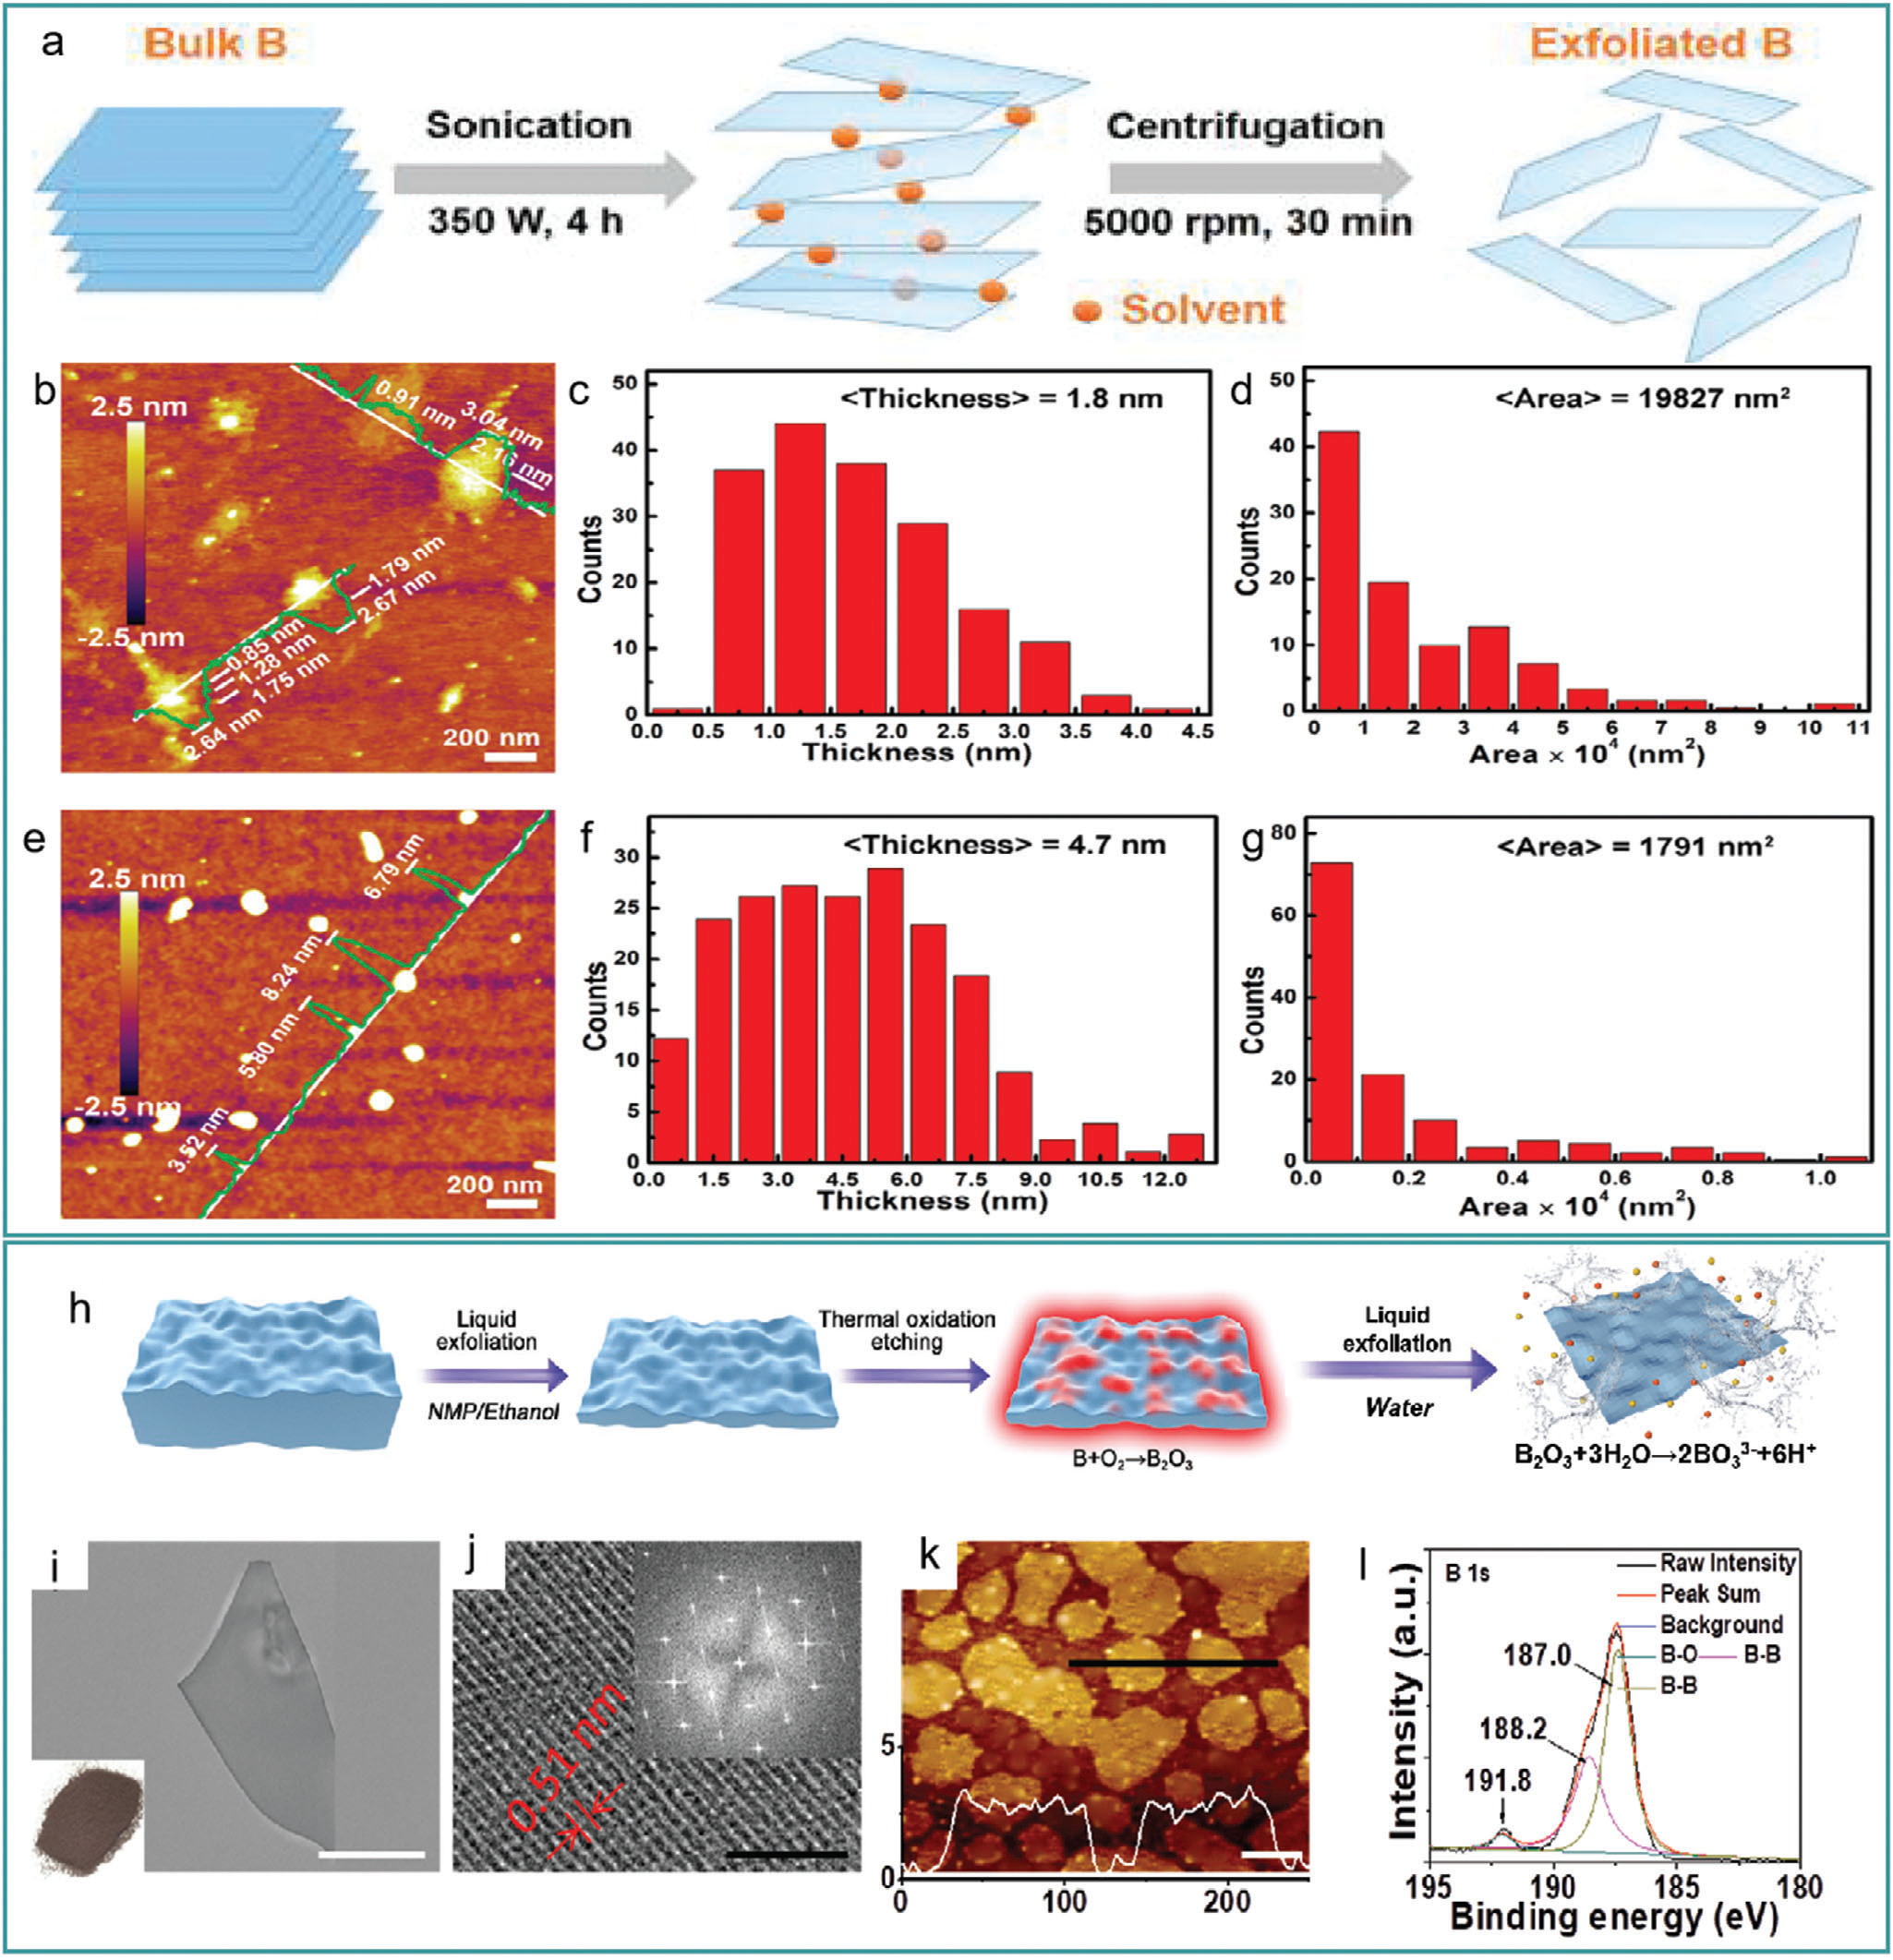
\includegraphics[width=0.7\linewidth]{AFM.png}
%     \caption{الف) شماتیک سنتز لایه برداری فاز مایع بوروفین های با کیفیت بالا به کمک فراصوت. b-g) خصوصیات AFM بوروفین سنتز شده در DMF (b-d) و IPA (e-g) توسط فراصوت. ب، ه) تصاویر توپوگرافی AFM و مشخصات ارتفاع. c,f,d,g) ضخامت و اندازه بوروفین آماده شده. الف – ز) تکثیر با اجازه.[86] حق چاپ 2018، انجمن شیمی آمریکا. ح) شماتیک اچینگ اکسیداسیون گرمایی و سنتز لایه برداری مایع بوروفین. i-l) تصاویر TEM، HRTEM، AFM، و طیف XPS بوروفین که با لایه برداری مایع در آب سنتز می شوند. نوار مقیاس سفید = 100 نانومتر و نوار مقیاس سیاه = 5 نانومتر. h–l) با اجازه تکثیر شده است.[25] حق چاپ 2018، Wiley-VCH.}
%     \label{fig:afm}
% \end{figure*}
% \subsubsection{سنتز روی \lr{Au (111)}}
% اخیراً \lr{Guisinger} و همکاران.\cite{kiralyBoropheneSynthesisAu2019}[85] \gls{Borophene} را با موفقیت روی یک زیرلایه \lr{Au(111)} سنتز کرد و تأثیر زیرلایه‌های \lr{Au(111)} با دمای متفاوت را بر رسوب گرمایی اتم‌های بور بررسی کرد. تصاویر \lr{SEM} از تمیز \lr{Au(111)} و \gls{Borophene} سنتز موفقیت آمیز \gls{Borophene} روی طلا را نشان دادند (شکل \ref{fig:cvdboro}\lr{4u,v}). بر خلاف سنتز \gls{Borophene} بر روی سوبستراهای \lr{Ag(111)}، \lr{Cu(111)} و \lr{Al(111)}، در زیرلایه \lr{Au(111)}، اتم های بور ابتدا در اتم های طلا در دماهای بالا (برابر یا بیشتر از 823 کلوین) حل می شوند. پس از سرد شدن به سطح جدا می شود و \gls{Borophene} را تشکیل می دهد (شکل \ref{fig:cvdboro}\lr{4s}). در فرآیند سنتز \gls{Borophene} بر روی یک زیرلایه \lr{Au(111)}، جزایر \gls{Borophene} نانومقیاس بر روی سطح Au(111) مشاهده شد (شکل \ref{fig:cvdboro}\lr{4v})، که از 1 تا 8 ساختار لوزی شکل 1 نانومتر مربع در مساحت سطح با یک \gls{Borophene} تشکیل شده است. 12 ساختار اتمی و هدایت فلزی (شکل \ref{fig:cvdboro}\lr{4t,w}). با افزایش غلظت بور، شبکه سه ضلعی شکسته شد و جزایر \gls{Borophene} بزرگتری را در سطح بستر تشکیل داد (شکل \ref{fig:cvdboro}\lr{4x}). بنابراین، بر اساس مطالعات فعلی، هرچه غلظت اتم بور بزرگتر باشد، اندازه \gls{Borophene} بزرگتر است. با این حال، کاربردهای بیشتر \gls{Borophene} به دلیل دشواری انتقال \gls{Borophene} از بسترهای فلزی محدود است.

% با توجه به پیوندهای ضعیف و انتقال بار محدود بین \lr{Au (111)} و \gls{Borophene} تشکیل شده بر روی سطح، \gls{Borophene} به راحتی جدا می شود که امکان کاربرد بیشتر را فراهم می کند. با این حال، تنها چند گزارش در مورد سنتز \gls{Borophene} در آزمایشگاه موجود است. همه نمونه‌های بالا از سنتز موفق \gls{Borophene} که تاکنون گزارش شده‌اند شامل روش‌های پایین به بالا هستند، به جز دو گزارش از سال 2018، که در آنها از روش‌های بالا به پایین استفاده شده است، همانطور که در زیر توضیح داده شده است.
% \subsection{سنتز بالا به پایین}
% تئو و همکاران.\cite{liScalableProductionFewLayer2018}[86] ثابت کرد که \gls{Borophene} چند لایه با کیفیت بالا با اندازه و ضخامت کنترل شده را می توان با لایه برداری فاز مایع به کمک اولتراسونیک سنتز کرد. در طول فرآیند سنتز، پودر بور در یک حلال دی متیل فرمامید \lr{(DMF)} / ایزوپروپیل الکل \lr{(IPA)} (1 میلی گرم در میلی لیتر) پراکنده شد و به مدت 4 ساعت در 350 وات فراصوت شد. \gls{Borophene} با ضخامت های مختلف با تنظیم سرعت سانتریفیوژ جمع آوری شد (شکل \ref{fig:afm}\lr{5a}). پس از آن، \gls{Borophene} به دست آمده توسط \lr{AFM} مشخص شد (شکل \ref{fig:afm}\lr{5b,e}). \gls{Borophene} جدا شده در \lr{DMF} دارای ضخامت متوسط 1.8 نانومتر و مساحت 19827 نانومتر بود (شکل \ref{fig:afm}\lr{5c,d})، در حالی که \gls{Borophene} جدا شده در \lr{IPA} دارای ضخامت 4.7 نانومتر و مساحت 1791 نانومتر بود (شکل \ref{fig:afm}\lr{5f,g}). بنابراین، اندازه و ضخامت \gls{Borophene} را می توان با تنظیم حلال مورد استفاده در لایه برداری اولتراسونیک کنترل کرد. جی و همکاران با الهام از خواص شیمیایی ویژه بور، که در آن \gls{Borophene} بی اثری در مقابل اکسیداسیون نشان می دهد، در حالی که لبه بیرونی آن و بور توده ای سه بعدی هر دو به راحتی اکسید می شوند.\cite{jiNovelTopDownSynthesis2018}[25] روش دیگری برای سنتز از بالا به پایین با استفاده از اچینگ در دمای بالا و سلب فاز مایع ایجاد کرد. پودر بور در یک حلال N-متیل پیرولیدون \lr{(NMP)} و الکل 1:1 پراکنده شد و به مدت 5 ساعت در 500 وات اولتراسونیک شد. سپس، صفحه های بور جدا شده و در یک ظرف سرامیکی حاوی اکسیژن در دمای 923 کلوین قرار داده شدند تا سطح دانه های بور به \ch{2B3O} اکسید شود. متعاقبا، از روش لایه برداری فاز مایع برای حل شدن سطح \ch{2B3O} در \ch{B3O} 3- استفاده شد (شکل \ref{fig:afm}\lr{5h}). در نهایت، \gls{Borophene} با اندازه مسطح ≈110 نانومتر و ضخامت کمتر از 3 نانومتر به دست آمد (شکل \ref{fig:afm}\lr{5i,k}). \gls{Borophene} حاوی حاشیه‌های تداخلی بود و گام راه راه آن 0.51 نانومتر بود که با ویژگی‌های ساختار بور $\beta$-لوزی وجهی مطابقت داشت (شکل \ref{fig:afm}\lr{5j}). طیف \lr{XPS} \gls{Borophene} (شکل \ref{fig:afm}\lr{5l}) سنتز موفقیت آمیز \gls{Borophene} را پس از لایه برداری لایه های اکسید شده در آب تایید کرد. این کار اولین گزارشی است که در مورد سنتز توده‌های بور به \gls{Borophene} با روشی از بالا به پایین بحث می‌کند، سطح ویژه \gls{Borophene} را تا حد زیادی بهبود می‌بخشد و کاربرد آن در دارورسانی را بهبود می‌بخشد. 3.3. عوامل کلیدی در سنتز \gls{Borophene} بر اساس نتایج تحقیقات نظری و سنتز تجربی، بستر، دما و حلال به عنوان عوامل کلیدی موثر بر تشکیل \gls{Borophene} نشان داده شده است. در ادامه، این عوامل کلیدی را به تفصیل تجزیه و تحلیل خواهیم کرد.

% \subsection{تأثیر بستر فلزی بر سنتز بوروفین}
% نظریه هسته‌زایی کلاسیک نشان می‌دهد که سد انرژی هسته‌زایی تشکیل مواد را تنظیم می‌کند، در حالی که مانع هسته‌زایی بور 2 بعدی بالاتر از ساختار \gls{bulk} سه بعدی آن است و از هسته‌زایی طبیعی \gls{Borophene} جلوگیری می‌کند.\cite{liuProbingSynthesisTwoDimensional2013, piazzaPhotoelectronSpectroscopyInitio2012, sergeevaB22B23AllBoron2012, kiranPlanartotubularStructuralTransition2005, ogerBoronClusterCations2007}[87-91] نقص‌های ترمودینامیکی. و پلی مورفیسم \gls{Borophene} دشواری سنتز آن را افزایش می دهد. بنابراین، کاهش سد هسته‌زایی بور دو بعدی و القای هسته‌زایی دوبعدی یک مسیر انرژی مطلوب برای سنتز \gls{Borophene} است.\cite{liEvolutionGrapheneGrowth2009}[92] در سال 2013، یاکوبسون و همکاران.\cite{liuProbingSynthesisTwoDimensional2013}[87] نشان داد که برهمکنش بین لایه‌های فلزی و بور به هسته‌زایی بورنن کمک می‌کند، زیرا مانع هسته‌زایی سه‌بعدی بور در برخی از بسترهای فلزی بالاتر از دو بعدی است.

% چه نوع بستری برای سنتز \gls{Borophene} مناسب است؟ دو معیار برای انتخاب زیرلایه‌های فلزی مناسب پیشنهاد شده است: باید حلالیت کمی در اتم‌های بور داشته باشد و نیروی اتصال بین بستر و اتم‌های بور باید متوسط باشد.\cite{liEvolutionGrapheneGrowth2009}[92] اگر نیرو بیش از حد قوی باشد، جدا کردن \gls{Borophene} از بستر دشوار است و \gls{Borophene} حتی ممکن است به راحتی یک بورید تشکیل دهد. به عنوان مثال، هنگامی که \gls{Borophene} بر روی بسترهای آهن، کو، یا نیکل سنتز می شود، \cite{vajeestonElectronicStructureBonding2001, burdettELECTRONICSTRUCTURETRANSITIONMETALBORIDES1986}[93،94] بورید می تواند به راحتی تشکیل شود. علاوه بر این، در زیرلایه های طلا، از آنجایی که برهمکنش بین اتم طلا و بور بسیار ضعیف است، بور غیرمسطح ممکن است به راحتی تشکیل شود.\cite{zhangTwoDimensionalBoronMonolayers2015}[95] با توجه به برهمکنش بین \gls{Borophene} و بستر فلزی، بسترهای رایج مورد استفاده را می توان به دو دسته عمده تقسیم کرد: یکی دارای انرژی اتصال قوی و انتقال بار زیاد با \gls{Borophene}، از جمله \lr{Mg(0001)}، \lr{Al(111)}، و \lr{Ti(0001)} است. \cite{hyamEffectParticleSize2008, cepekEpitaxialGrowthMgB22004}[96،97] مشخصات نوارهای $\sigma$ (داخلی) \gls{Borophene} شش ضلعی سنتز شده روی این بسترها، به جز تغییر سطح فرمی، شبیه به فاز ایستاده آن است. دیگری انرژی پیوند نسبتاً پایین‌تری با \gls{Borophene} دارد، از جمله \lr{Au(111)} و \lr{Ag (111)}، و باندهای درون صفحه \gls{Borophene} شش ضلعی به زیر باندهای زیادی تقسیم می‌شوند.\cite{zhangBoronSheetAdsorbed2012}[98] خو و همکاران \cite{xuNucleationGrowthBorophene2016}[99] به طور نظری مکانیسم هسته‌زایی و فرآیند رشد \gls{Borophene} را در سطح \lr{Ag(111)} ارزیابی کرد و تأیید کرد که ساختار پایدار بهینه، ساختاری است که \lr{HHs} به‌طور موازی مرتب شده‌اند و غلظت \lr{HHs} با آزمایش 1/6 بود. ژائو و همکاران \cite{liuBoronClusterTwoDimensional2013}[100] دریافتند که خوشه های بور متراکم دوبعدی به راحتی روی سطح مس (111) تشکیل می شوند. علاوه بر این، هر چه اندازه خوشه بزرگتر باشد، انرژی تشکیل کوچکتر است. بنابراین، بسترهای فلزی تفاوت زیادی در ساختار \gls{Borophene} ایجاد شده ایجاد می کنند و انتخاب یک بستر مناسب با توجه به محصول مورد نظر اهمیت ویژه ای دارد.

\section{خواص بوروفین}
\subsection{خواص شیمیایی}
نشان داده شده است که بور دو بعدی نسبت به اکسیداسیون بی اثر است، در حالی که لبه بیرونی آن و بور \gls{bulk} سه‌بعدی کمتر است.\cite{fengExperimentalRealizationTwodimensional2016} بور دارای سه الکترون ظرفیت است $[\text{He}]2S^22P^1$. با این حال، یک الکترون ارتقا یافته از اوربیتال $\text{2S}$ به $\text{2P}$ می تواند بور را قادر سازد که چهار اوربیتال ظرفیت در دسترس داشته باشد. بنابراین، تعداد الکترون‌های ظرفیت کمتر از تعداد اوربیتال‌های ظرفیت است و اوربیتال‌های الکترونی را نمی‌توان به طور کامل با الکترون‌های اتم بور در هنگام تشکیل پیوندهای شیمیایی پر کرد و منجر به تشکیل اتم‌های بور فاقد الکترون می شود. ترکیب اتم‌های بور سه‌بعدی \gls{bulk} واتم‌های بور دو بعدی در اطراف محیط، هر دو بر اساس پیوندهای دو الکترونی کلاسیک دو مرکزی هستند، اما اتم‌های داخلی پیوندهای دو الکترونی چند مرکزی بورون دوبعدی ناجایگزیده شده‌اند که منجر به تفاوت آنها در پایداری اکسیداسیون می‌شود. \cite{zhangTwodimensionalBoronStructures2017} به عنوان مثال، در یک صفحه بور، \glsdesc{HH} ها به عنوان "\gls{acceptors}" عمل می کنند و اتم های بور در مرکز شش ضلعی‌ها به عنوان "\gls{donors}" عمل می کنند، بنابراین کمبود الکترون در بور را جبران می کنند و صفحه های بور را نسبت به اکسیداسیون بی اثر می کنند.[51] \gls{Wu} و همکاران\cite{fengExperimentalRealizationTwodimensional2016} از طیف‌سنجی فوتوالکترون پرتو ایکس (\gls{XPS}) برای تشخیص ترکیب شیمیایی \gls{Borophene} تک‌لایه استفاده کرد و نشان داد که دو پیک انرژی کم‌پیوند (\lr{188.2} و \lr{187.1 eV}) از دو پیوند \ce{B-B} مختلف در صفحه‌های بور دو بعدی هستند، در حالی‌که انرژی پیوند پیک $1s$ در بور \gls{bulk} سه‌بعدی به طور کلی \lr{≈189-190 eV} است. با این حال، پیک انرژی بالاتر \lr{(191.5 eV)} قرار است از اتم بور اکسید شده ناشی شود، بر اساس پیک‌های بور اکسید شده قبلا گزارش شده است.
  
از طریق محاسبه و مقایسه مساحت پیک، مشاهده شد که نسبت اتم بور اکسید شده به اتم بور اکسید نشده تنها 0.23 است که نشان می‌دهد اکثر اتم‌های بور روی سطح \gls{Borophene} دارای ثبات خاصی در برابر اکسیداسیون هستند. علاوه بر این، اتم های اکسید شده عمدتاً در لبه صفحه \gls{Borophene} قرار دارند که می تواند با آزمایش‌های \gls{STM} درجا تأیید شود. اکسیژن به طور مستقیم به محفظه خلاء پمپ شد و سطح بور درجا با استفاده از \gls{STM} اسکن شد. در غلظت‌های بالای اکسیژن، لکه‌های روشن در لبه‌های جزیره بور ظاهر می‌شوند که نشان می‌دهد اتم‌های بور شروع به اکسید شدن کرده‌اند، در حالی که تراس صفحه‌های بور تغییر کمی نشان می‌دهد. با ادامه جریان اکسیژن، صفحه‌های بور پایدار ماندند و فاز \gls{striated} هنوز قابل مشاهده بود، که نشان می‌دهد اکسیداسیون بور عمدتاً در لبه‌ها اتفاق می‌افتد، در حالی که صفحه بور خود در برابر اکسیداسیون پایدار است. بنابراین، \gls{Borophene} دو بعدی در مقایسه با بور \gls{bulk} سه بعدی نسبت به اکسیداسیون بی اثرتر است. علاوه بر این، \gls{Guisinger} و همکاران.\cite{mannixSynthesisBorophenesAnisotropic2015} همچنین دریافتند که حالت اکسیداسیون در \gls{Borophene} زمانی که در معرض شرایط محیطی قرار می‌گیرد تشخیص داده می‌شود، اما اکسیداسیون عمدتاً در لبه‌های \gls{Borophene} به دلیل حالت‌های لبه فعال آن رخ می‌دهد. با وجود قرار گرفتن در معرض دوز بالای اکسیژن، مناطق با شبکه کامل تقریبا دست نخورده باقی می مانند.\cite{zhaiObservationAllboronFullerene2014} با این وجود، \gls{Guisinger} و همکاران همچنین نشان داد که \gls{Borophene} به اندازه مواد دوبعدی دیگر از نظر شیمیایی پایدار نیست و زمانی که برای مدت طولانی در معرض هوا قرار می‌گیرد می‌تواند مستعد آلودگی باشد. این پایداری شیمیایی، اگرچه قابل مقایسه با گرافین نیست، به حل مشکل ناپایداری در برابر اکسیداسیون در مواد دو بعدی کمک می کند. علاوه بر این، پایداری \gls{Borophene} در برابر اکسیژن را می توان با به عنوان مثال، مهر و موم کردن \gls{Borophene} از اکسیژن با پوشاندن مواد دیگر افزایش داد، و همچنین ثابت کردند که یک لایه درپوش اکسید سیلیسیم/سیلیکا می تواند تا حد زیادی مانع اکسیداسیون \gls{Borophene} شود که منجر به مطالعه بیشتر ما می شود. در مورد مقاومت اکسیداسیون بور دو بعدی.\cite{zhangTwodimensionalBoronStructures2017} از سوی دیگر، با فعالیت شیمیایی لبه‌های \gls{Borophene}، می‌تواند واکنش‌های تکامل هیدروژن را کاتالیز کند؛ \cite{zhangTwoDimensionalBoronMonolayers2015} این ویژگی جالب نه تنها امکان جدیدی را برای توسعه انرژی جایگزین فراهم می‌کند، بلکه مسیرهای جدیدی را برای کاربرد بور باز می‌کند.

\subsection{ویژگی های مکانیکی}
\gls{Borophene}، ساخته شده از پیوندهای کووالانسی چند مرکزی به جای پیوندهای کووالانسی کلاسیک دو مرکزی موجود در سایر مواد دو بعدی معمولی، نوید خواص مکانیکی استثنایی را می دهد. پیوندهای کوولانسی $\sigma$ در صفحه با انرژی بستگی $5.09\; eV \approx$  یکی از قوی‌ترین پیوندها در طبیعت هستند که منجر به استحکام بسیار بالا و پایداری ساختاری عالی \gls{Borophene} می‌شود. در مورد \gls{Borophene}، علاوه بر پیوندهای کووالانسی کلاسیک که استحکام مهمی به صفحه می دهد، پیوندهای فلزی مانند چند مرکزی به طور کلی به ساختار سیالیت بالقوه می بخشند.\cite{zhangTwoDimensionalBoronMonolayers2015} بعلاوه، به عنوان یک ماده دو بعدی، \gls{Borophene} به دلیل ضخامت اتمی، انعطاف پذیری بسیار خوبی از خود نشان می دهد. علاوه بر این، طبق پیش‌بینی‌ها، \gls{Borophene} در یک \gls{strain} بزرگ تحت یک انتقال فاز ساختاری قرار می‌گیرد که منجر به \gls{toughness} مکانیکی بالاتر می‌شود. علاوه بر این، \gls{Wang} و همکاران\cite{wangStrainEffectsBorophene2016} ثابت کرد که از آنجایی که پیوندهای \ce{B-B} هنگام افزایش \gls{strain} کششی ضعیف می شوند، نسبت پواسون در امتداد جهت خارج از صفحه منفی است\cite{liuRecentProgressGrapheneanalogous2019}.

نشان داده شده است که \gls{stiffness} درون صفحه $\nu_{1/6}$ \gls{Borophene} کمتر از بسیاری از مواد دو بعدی مانند گرافین است\cite{zhangElasticityFlexibilityIdeal2017}. محاسبه شد که عدد \gls{Foppl-von Karman} در واحد سطح صفحه $\nu_{1/6}$ که به صورت \lr{C/D} تعریف می شود، یعنی نسبت بین مدول درون صفحه و \gls{stiffness} خمشی، که در بین مواد ذکر شده در آن تحقیق بالاترین است. بنابراین، یکی از منعطف ترین مواد با سطوح بالایی از انعطاف پذیری در برابر تغییر شکل خارج از صفحه است. \gls{Borophene} را می توان بر اساس هندسه اتمی آن، شامل صفحه های مثلثی ($\nu_0$)، صفحه های $\alpha$ ($\nu_{1/9}$)، $\nu_{1/5}$، $\nu_{1/6}$، $\nu_{1/7}$، $\nu_{1/8}$، $\nu_{1/10}$ و $\nu_{12}$ طبقه بندی کرد \cite{zhaoPhononmediatedSuperconductivityBorophenes2016}. صفحه‌های مثلثی \gls{relaxed} به دلیل وجود الکترون‌های زیاد، ساختار کمانشی مانند تخته‌شویی را نشان می‌دهند، در حالی که صفحه‌های $\nu_{1/5}$، $\nu_{1/6}$ و سایر صفحات به دلیل غلظت بالای \glsdesc{HH} که منجر به کمبود الکترون در خلاء می‌شود، کاملاً مسطح هستند. ساختار مسطح ناپایداری ناشی از ساختار کمانش صفحه بور مثلثی را حل می کند. 

همانطور که در بالا ذکر شد، ورود \glsdesc{HH} به \gls{Borophene} می تواند به طور موثر ساختار را تثبیت کند، زیرا \gls{strain} اعمال شده در نزدیکی \glsdesc{HH} بسیار متمرکز است، که کشسانی کل صفحه‌ها را کنترل می کند. از سوی دیگر، افزایش غلظت \glsdesc{HH} می تواند سطح صفحه را گسترش دهد، در نتیجه کشش را کاهش می دهد، و انتقال فاز ساختاری تجربه شده توسط \gls{Borophene} می تواند مواد را سخت تر کند و در برابر بارهای بزرگ حتی در کشش شدید مقاومت کند. بنابراین، \glsdesc{HH} ها برای فرآیند شکستن انعطاف پذیر \gls{Borophene} حیاتی هستند. با این وجود، \glsdesc{HH} ها به طور قابل توجهی بر خواص مکانیکی مواد تأثیر می گذارند. افزایش \glsdesc{HH} باعث کاهش تعداد پیوندهای \ce{B-B} و در نتیجه سختی مواد می شود. استحکام کششی نهایی شبکه بور نیز به شدت تحت تأثیر قرار خواهد گرفت. به عبارت دیگر، با اضافه کردن \glsdesc{HH} ها، با وجود افزایش $\eta$، تغییرات \gls{stiffness} \gls{Borophene} محدود می شود. 

با توجه به روش \gls{atomic displacement}، \cite{zhangElasticityFlexibilityIdeal2017, schabelENERGETICSINTERPLANARBINDING1992, wangStrainEffectsBorophene2016}. $\nu_{1/6}$ پیش‌بینی شده است که دارای استحکام ایده‌آل 16.4 نیوتن بر متر است که علیرغم اینکه به خوبی صفحه‌های گرافین و نیترید بور شش ضلعی \ce{h-BN} نیست، بالاتر از سایر مواد دو بعدی، مانند \ce{MoS2} \cite{liIdealStrengthPhonon2012, zouPredictingDislocationsGrain2013}و فسفرن\cite{weiSuperiorMechanicalFlexibility2014} است. علاوه بر این، \gls{stiffness} خمشی و نسبت پواسون نیز به شدت به چگالی \glsdesc{HH} بستگی دارد. بنابراین، این پارامترهای مکانیکی را می توان به طور انعطاف پذیر با توجه به الزامات برنامه‌های مختلف تغییر داد \cite{zhangElasticityFlexibilityIdeal2017}.

مکانیسم ناپایداری \gls{Borophene} نیز ارزیابی شد، \cite{wangStrainEffectsBorophene2016, zhongElectronicMechanicalProperties2018, weiSuperiorMechanicalFlexibility2014, zouPredictingDislocationsGrain2013} که نشان می‌دهد مکانیسم شکست، ناپایداری الاستیک تحت یک \gls{strain} تک محوری در جهت زیگزاگ است، در حالی که برای \gls{strain} تک محوری در امتداد جهت ارمچیر و \gls{strain} دو محوره، مکانیسم شکست به فونون نسبت داده می‌شود. \gls{Borophene} به عنوان یک ماده دو بعدی با انعطاف پذیری بی سابقه، استحکام ایده‌آل بالا و خاصیت ارتجاعی عالی پتانسیل بالایی در تهیه مواد کامپوزیتی و دستگاه‌های انعطاف پذیر دارد. این داده‌ها نشان می دهد که خواص \gls{Borophene} را می توان با تنظیم غلظت \glsdesc{HH} و تسلط بر مکانیسم ناپایداری \gls{Borophene} تنظیم کرد.

\section{خواص الکتریکی:}
با ماهیت کمبود الکترون عنصر \lr{B}، پایدارترین ساختار مخلوطی از ساختارهای شش ضلعی و مثلثی \cite{tangNovelPrecursorsBoron2007} با پیوندهای دو و سه مرکز است. دارای خواص الکتریکی نسبتا منحصر به فردی مانند فلزی بودن، اثرات دیراک فرمی، ابررسانایی و نیمه رسانایی است.
\subsection{فلزی بودن:}
یاکوبسون و همکاران \cite{penevCanTwoDimensionalBoron2016} از نظر تئوری پیش‌بینی کردند که همه پلی‌مورف‌های \gls{Borophene} فلزی هستند، متفاوت از خواص نیمه‌رسانا یا عایق آلوتروپ‌های \gls{bulk} سه‌بعدی، که تنها بخش کوچکی از آن‌ها می‌توانند تحت فشار فوق‌العاده به فلز تبدیل شوند \cite{eremetsSuperconductivityBoron2001}. پس از آن، به طور تجربی تایید شد که فلزی بودن توسط مدار $p_z$ تعیین می‌شود \cite{shangTwoDimensionalBoron2018}. \gls{Wu} و همکاران \cite{fengExperimentalRealizationTwodimensional2016} از \gls{scanning tunneling spectroscopy} برای اندازه‌گیری حالت‌های الکترونی فازهای $\beta_{12}$ و $\chi_3$ با موفقیت استفاده کرد و دریافت که چگالی‌های جایگزیده حالت‌ها در اطراف سطح فرمی وجود دارد که ساختار نوار انرژی فلزی بودن را بیشتر نشان می‌دهد. \gls{Matsuda} و همکاران \cite{fengDirectEvidenceMetallic2016} باندهای مشتق از بور فلزی $\beta_{12}$ را با استفاده از طیف‌سنجی فوتوالکترون با تفکیک زاویه مشاهده کردند و یک پدیده جالب را استنباط کردند - همزیستی پاکت‌های الکترونی و حفره‌ای در سطح فرمی - طبق محاسبات اولیه، که فلزی بودن آن را نیز نشان می‌دهد. علاوه بر این، \gls{Fazzio} و همکاران \cite{padilhaDirectionalDependenceElectronic2016} تایید کرد که رسانایی \gls{Borophene} ناهمسانگرد است و انتقال جریان در دو جهت عمود بر هم وابسته است.
\subsection{خواص توپولوژیکی}
مواد توپولوژیکی بسیاری از خواص کوانتومی جدید، متفاوت از مواد سنتی را نشان می‌دهند \cite{qiTopologicalInsulatorsSuperconductors2011}، و با توجه به ساختارهای الکترونی می‌توان آنها را به سه نوع تقسیم کرد، یعنی عایق‌های توپولوژیکی، \cite{hsiehTopologicalCrystallineInsulators2013}  \gls{Weyl semimetal} توپولوژیکی، \cite{xuDiscoveryWeylFermion2015} و \gls{Dirac semimetal} دیراک توپولوژیکی \cite{wanTopologicalSemimetalFermiarc2011}. \gls{Dirac semimetal} توپولوژیکی ساختار الکترونی منحصر به فردی را نشان می دهد که در آن نوارهای انرژی نزدیک به سطح فرمی دارای نقاط دیراک سه بعدی هستند و سه جهت حرکت مجاور اطراف نقاط دیراک همگی روابط پراکندگی خطی هستند. چنین ویژگی‌های تقطع نواری توسط تقارن کریستالی محافظت می‌شوند، که باعث می‌شود چشم‌انداز کاربردی بسیار جذابی در دستگاه‌های الکترونیکی، نیمه‌رساناها و سایر زمینه‌ها داشته باشند \cite{zhaoPalgraphynePromising2D2020}. در حالی که مواد دیراک توپولوژیکی کشف شده تاکنون معمولاً حاوی عناصر فلزی سنگین هستند که با مشکلات سختی روبرو هستند که برای کاربردهای عملی رسانا نیستند، به عنوان مثال، آلودگی محیطی، هزینه بالا و ایمنی مواد. بنابراین، بررسی عناصر سبک برای ترکیب مواد توپولوژیکی پایدار ضروری است. گرافین ماده معمولی سبک دیراک است که بسیاری از پدیده های فیزیکی جدید و خواص الکترونی که توسط محققان مشاهده شده توسط مخروط های دیراک ارائه شده است. امروزه مواد دیراک دیگر محدود به مواد کربنی نیستند، بلکه مواد مختلف دیگری را نیز پوشش می دهند \cite{novoselovElectricFieldEffect2004}. بور به عنوان عنصر سبک سمت چپ اتم کربن، پتانسیل زیادی برای تولید مواد دیراک دو بعدی با خواص مشابه در مقایسه با مواد کربنی در بسیاری از جنبه‌ها دارد. 

با آزمایش‌ها تأیید شده که، \cite{fengDiracFermionsBorophene2017} $\beta_{12}$ و $\chi_3$ \gls{Borophene} هر دو میزبان مخروط‌های دیراک هستند، در حالی که \gls{Borophene} کاملاً هیدروژنه شده، مانند \lr{Pmmn} و \lr{Cmmm}، مخروط‌های دیراک پیچ خورده را با سرعت فرمی فوق‌العاده بالا $(3.5 \times 106\; m s^{-1})$ نشان می‌دهند که حدود چهار برابر گرافین ($8.2\times 105\; m s^{-1}$)؛ \cite{xuHydrogenatedBoropheneStable2016, hwangFermiVelocityEngineering2012, trevisanuttoInitioGWManyBody2008}، است. با این حال، هر دو مخروط دیراک آنها از نظر شکل کامل نیستند، که منجر به خواص انتقال ناهمسانگرد بروفین می شود. وجود مخروط‌های دیراک نشان می‌دهد که \gls{Borophene} می‌تواند اثرات کوانتومی جالبی را از خود نشان دهد، انتظار می‌رود که یک ماده عنصری خالص با اثر دیراک-فرمی جرمی صفر باشد \cite{malkoCompetitionGrapheneGraphynes2012, zhouSemimetallicTwoDimensionalBoron2014} و چشم‌اندازی در کاربرد الکترونی دردستگاهای با سرعت بالا و کم مصرف در مقیاس نانو داشته باشد.

در سال 2014، \gls{Wang} و همکاران \cite{zhouSemimetallicTwoDimensionalBoron2014} از روش جستجوی ساختار تکاملی \gls{ab initio} استفاده کردند و یک نوع \gls{Borophene} به نام \lr{Pmmn} \gls{Borophene} با فرمیون‌های دیراک بدون جرم، که دارای مخروط دیراک پیچ خورده است، ارائه کردند \cite{li2018review}. به طور شگفت انگیزی، \lr{Pmmn} سومین ماده فلزی دیراک و اولین ماده بور دو بعدی دیراک است. متعاقباً، یک صفحه بور نیمه یونی دوبعدی به نام $\gamma-B_{28}$ توسط \gls{Du} و همکاران گزارش شده است، \cite{maGraphenelikeTwoDimensionalIonic2016} که شامل صفحه گرافین مانند و جفت $B_2$ است که بین آنها یک انتقال بار قوی وجود دارد و مخروط‌های دوگانه دیراک بدون جرم را نشان می دهد سرعت فرمی بالاتر از گرافین، که پایداری انرژی \gls{Borophene} \lr{P6/mmm} را افزایش می‌دهد. 

خواص توپولوژیکی $\beta_{12}$ \gls{Borophene} موضوع داغ بوده است زیرا با موفقیت در \lr{Ag(111)} سنتز شد.\cite{mannixSynthesisBorophenesAnisotropic2015} متعاقبا، \gls{Matsuda} و همکاران \cite{fengDiracFermionsBorophene2017}. 
\begin{figure*}
    \centering
    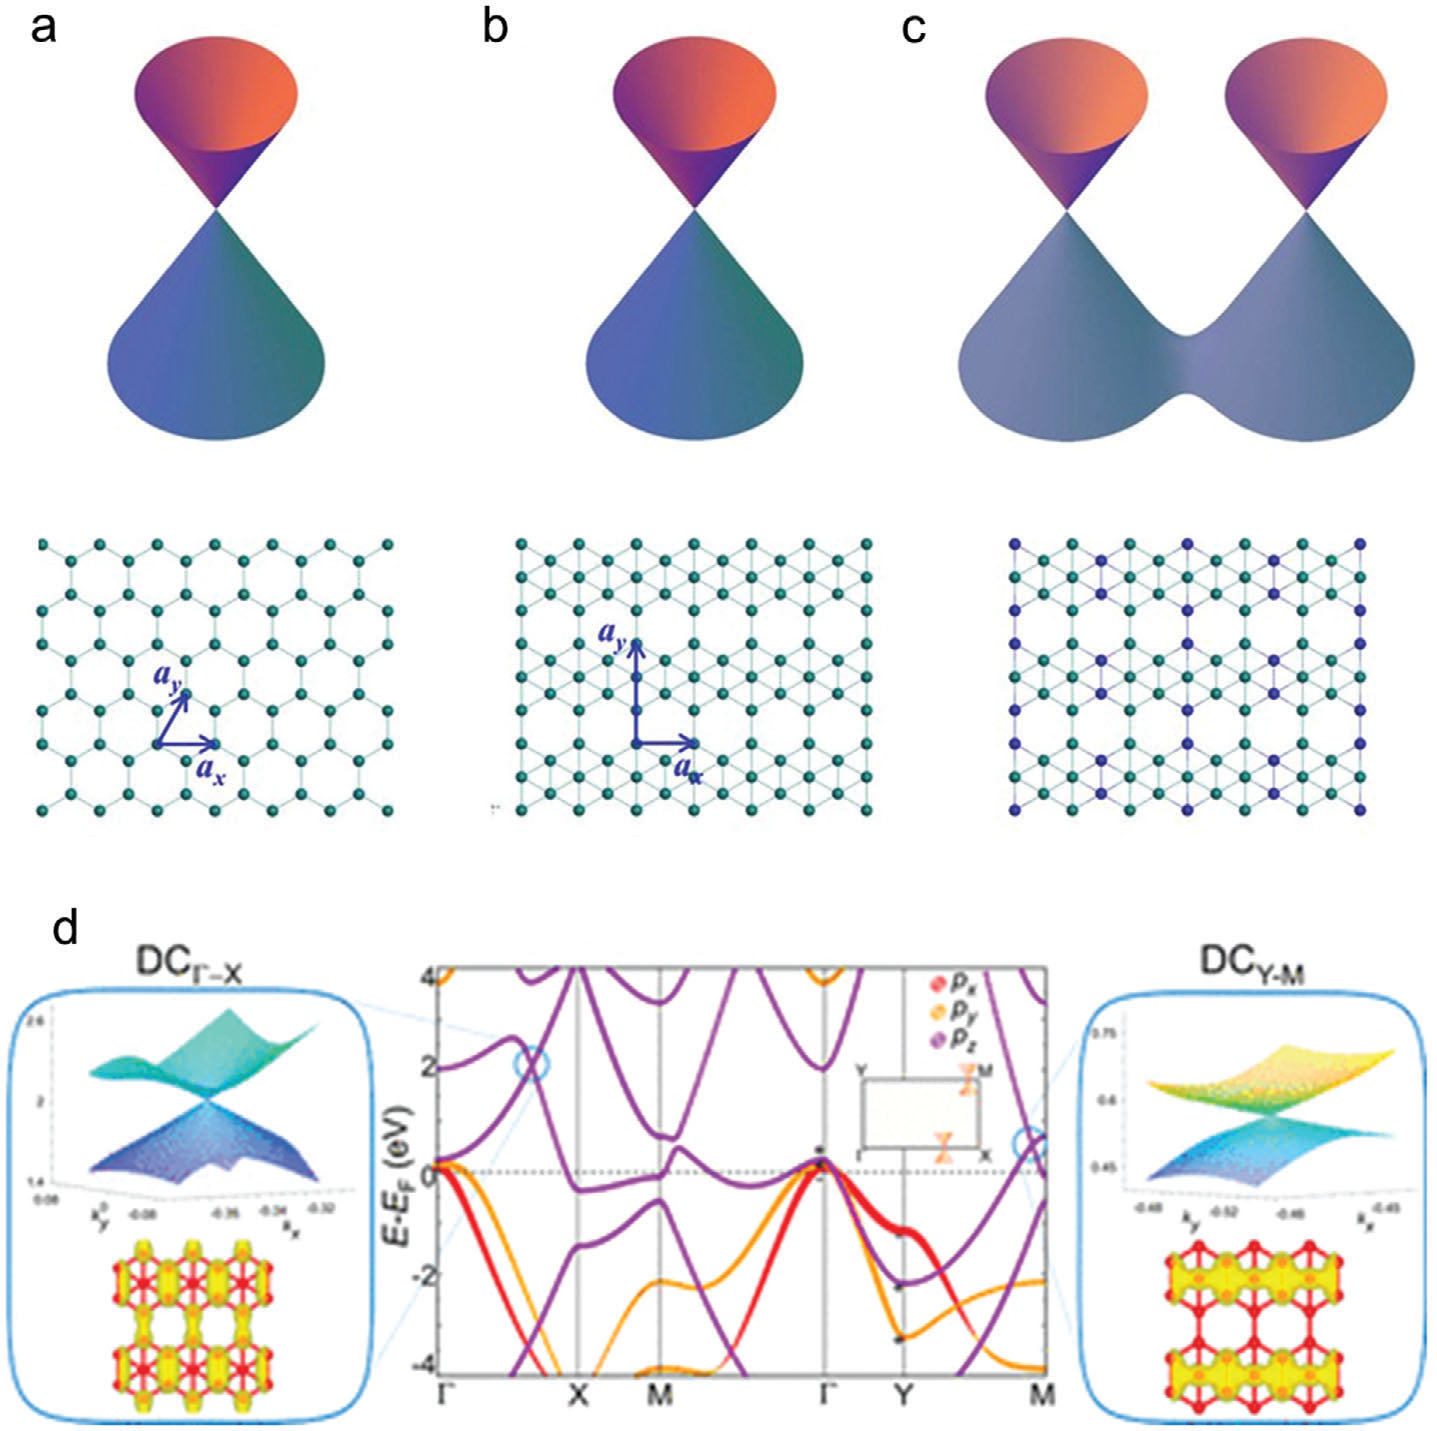
\includegraphics[width=0.7\linewidth]{Diraccone.png}
    \caption{مخروط‌های دیراک و شبکه‌های الف) بوروفین لانه زنبوری. ب) بوروفین $\beta_{12}$. ج) بوروفین} $\beta_{12}$ با اختلال $3\times 1$. الف – ج). د) ساختار نواری بوروفین $\beta_{12}$ (مرکز)، و نمای سه‌بعدی مخروط دیراک ($DC_{\Gamma-X}$، سمت چپ) و مخروط دیراک ($D_{CY-M}$، سمت راست) با نمودار چگالی ایزوشارژ تجزیه‌شده نواری
    \label{fig:Diraccone}
\end{figure*}
ابتدا با محاسبات اولیه در سال 2017 تأیید کردند که $\beta_{12}$ \gls{Borophene} دارای فرمیون‌های دیراک است که به طور تجربی اولین ماده دیراک تک لایه غیر لانه زنبوری را تأیید کرد. گزارش شده است که نوارهای $\pi$ نزدیک سطح فرمی $\beta_{12}$ \gls{Borophene} از مدار $p_z$ مانند گرافین جدا شده است. علاوه بر این، تنها با در نظر گرفتن مدار $p_z$ روی \gls{Borophene} $\beta_{12}$ مستقل، مخروط‌های دیراک در $(±2\pi/3a،0)$ از اولین منطقه بریلوین \lr{(BZ)} در \gls{Borophene} $\beta_{12}$ مستقل از طریق یک مدل اتصال محکم ساده آشکار شدند. مشابه شبکه لانه زنبوری، $\beta_{12}$ \gls{Borophene} را می توان به دو زیرشبکه مثلثی تجزیه کرد و در نتیجه مخروط دیراک میزبان، و شکافتن مخروط های دیراک تحت تأثیر تقارن زیرشبکه قرار می گیرد (شکل \ref{fig:Diraccone}الف-ج). در همین حال، \gls{Matsuda} و همکاران همچنین پیشنهاد کرد که هر مخروط دیراک را می‌توان با استفاده از اختلالات تناوبی تقسیم کرد و مخروط‌های شکافته دیراک غیر متمرکز هستند و با گرافین متفاوت هستند. \gls{Gupta} و همکاران \cite{guptaDiracConesNodal2018} منشا فرمیونهای دیراک را به ترتیب در $\beta_{12}$ روی \lr{Ag(111)} و $\beta_{12}$ بوروفین مستقل کاوش کرده اند. بر اساس گزارش آنها، یک خط گره دیراک از نظر توپولوژیکی و دو مخروط دیراک در $\beta_{12}$ \gls{Borophene} وجود دارد که در میان آنها دو مخروط دیراک به ترتیب در امتداد جهت‌های $\Gamma-X$($DC_{\Gamma-X}$) و $Y-M$ ($DC_{Y-M}$) قرار دارند. شکل \ref{fig:Diraccone}.د). بعلاوه، اگرچه مخروط های دیراک \gls{Borophene} $\beta_{12}$ با پشتیبانی \lr{Ag(111)} می توانند شکاف ایجاد کنند. خط گره هنوز از نظر توپولوژیکی محافظت می شود. حالت‌های توپولوژیکی بی‌اهمیت در این $\beta_{12}$ \gls{Borophene} می‌توانند از درک بیشتر خواص توپولوژیکی \gls{Borophene} حمایت کنند، و بنابراین به نفع ایفای نقش در تحقیقات و کاربردهای پایه هستند. در سال 2017، \gls{Chen} و همکاران \cite{zhangDiracNodalLines2017} یک ساختار بور دو بعدی جدید به نام \ce{hr-sB} با دو نوع فرمیون دیراک مربوط به خط گره دیراک و مخروط های دیراک گرادیان ناهمسانگرد قوی جدا از هم، متفاوت از مخروط های دیراک سنتی مشاهده شده در $\beta_{12}$ پیش بینی کرد. با الهام از ساختار لانه زنبوری در گرافین، تحقیقات مربوط به مخروط‌های دیراک بور درون صفحه‌ای لانه زنبوری نیز جذاب است. علاوه بر این، یک اکسید \gls{Borophene} لانه زنبوری به نام \ce{h-B2O} که اخیراً یافت شده است، دارای رسانایی عالی به عنوان فلز حلقه گره‌ای توپولوژیکی دوبعدی است و بنابراین یک ماده آند بسیار امیدوارکننده برای باتری‌هایی با ظرفیت بسیار زیاد است \cite{hu2DHoneycombBorophene2020}. 

امروزه مطالعات مربوط به خواص توپولوژیکی به مدل فرمیون های ویل یا دیراک محدود نمی شود و تجزیه و تحلیل تقارن به کریستال های دارای نظم مغناطیسی و برهمکنش‌ها نیز کشیده شده است \cite{bradlynDiracWeylFermions2016}. اخیراً \lr{Ezawa} و همکاران \cite{ezawaTripletFermionsDirac2017} پیشنهاد کرد که ممکن است فرمیون های سه گانه در $\beta_{12}$ بوروفین وجود داشته باشد و تئوری های سه باندی برای فرمیون های سه گانه ساخت. همه درک بالا از خواص توپولوژیکی مواد بور دوبعدی، پایه محکمی را برای تحقیقات بعدی کاربرد الکتریکی ایجاد می کند.\cite{fanCatScradlelikeDirac2018}
\subsection{ابررسانایی}
گزارش شده است که جرم اتمی نسبتاً کم بور می تواند جفت الکترون-فونون قوی ایجاد کند، و فلزی بودن \gls{Borophene} می تواند باعث ایجاد غلظت حامل بالاتری شود، \cite{kortusSuperconductivityMetallicBoron2001, choiOriginAnomalousSuperconducting2002, anSuperconductivityMgB2Covalent2001} که هر دو از عوامل کلیدی در تشکیل ابررساناهای معمولی هستند. ، ثابت می کند که \gls{Borophene} پتانسیل تبدیل شدن به یک ابررسانا را دارد. شایان ذکر است، \gls{Yakobson} و همکاران \cite{penevCanTwoDimensionalBoron2016} دمای بحرانی آن را $T_c$ نسبت به گرافین پیش بینی کرد ($T_c \approx 8.1\; K$ در تئوری \cite{profetaPhononmediatedSuperconductivityGraphene2012} و از نظر تجربی $4.5\;K$ \cite{xueSuperconductivityPotassiumDopedFewLayer2012}) با این وجود، \gls{doped} الکترون و \gls{strain} کششی می‌توانند باعث سرکوب ابررسانایی برای \gls{Borophene} شوند، \cite{chengSuppressedSuperconductivitySubstratesupported2017, xiaoEnhancedSuperconductivityStrain2016}\cite{wuLithiumBoronLiBMonolayers2016} که تشخیص دمای بحرانی \gls{Borophene} در آزمایش‌ها را دشوار می‌سازد. با این حال، هنگامی که به این مسائل پرداخته شد، این ویژگی‌ها انعطاف پذیری طراحی و راحتی برای \gls{Borophene} را در دستگاه های ابررسانا افزایش می دهد.
\subsection{نیمه رسانایی}
دانشمندان به طور تجربی نشان داده‌اند که چندین فاز \gls{Borophene} به دلیل وجود \gls{bandgap} غیرصفر دارای نیمه‌رسانایی هستند. دریافتند که صفحات $\alpha$و $\alpha^{\prime}$ (صفحه کمی کمانش شده) هر دو نیمه هادی‌های با \gls{bandgap} با فاصله باند غیرمستقیم 1.40 و $1.10\; eV$ هستند که در میان آنها صفحه $\alpha^{\prime}$ بیشترین انرژی \gls{cohesive} را دارد و احتمالاً بیشترین انرژی \gls{cohesive} را دارد. \gls{Borophene} کماندار پایدار \gls{Kou} و همکاران \cite{kouHighmobilityAnisotropicTransport2016} دریافتند که اگرچه حداقل است، اما باز هم می توان با تغییر تنش اعمال شده، شکاف باند سطح \gls{Borophene} ضخیم تر را تغییر داد، که باعث تغییر بیشتر در تحرک الکترون و در نتیجه تبدیل نوع رسانایی \gls{Borophene} از فلزی به نیمه هادی می شود. در این حالت، تحرک الکترون بالاتری را می توان با تغییر تنش اعمال شده به دست آورد. بنابراین، $\gamma-B_{28}$ \gls{Borophene} دارای چشم انداز کاربردی در زمینه دستگاه‌های حساس به فشار و حساس به نور است.

\subsection{حالت های الکترونی تقریباً آزاد یک بعدی:}
حالت‌های تقریباً الکترون آزاد \gls{NFE} که با جرم مؤثر تقریباً مطابق با جرم الکترون آزاد ($m_e$) مشخص می‌شوند \cite{eknapakulNearlyfreeelectronSystemMonolayer2016, fengElectronicPropertiesSuperatom2011}، پراکندگی انرژی سهموی را نشان می‌دهند ، که خواص انتقال الکترون آن نسبتاً قابل‌توجه است و می‌تواند در گسیل‌کننده‌های الکترون اعمال شود \cite{chenNonlocalChemicalReactivity2009, csanyiRoleInterlayerState2005}. حالت‌های \gls{NFE} می‌توانند به طور گسترده روی سطوح مواد با ابعاد کم که پتانسیل محصور شدن به آنها عمود است وجود داشته باشند، مانند مولکول‌های صفر بعدی \ce{C60}، \cite{zhaoSuperatomStatesFullerenes2009, fengAtomlikeHollowcoreboundMolecular2008} نانولوله‌ها و نانوروبان‌های یک بعدی، \cite{yamanakaElectronInjectionNearly2014, huNearlyFreeElectron2010} و گرافین دو بعدی، \cite{silkinImagePotentialStates2009} در حالی که به دلیل وجود گرادیان پتانسیل معمولاً به صفحه پایه ماده عمود است، این حالت‌های \gls{NFE} ترجیح می دهند به جای ماندن در اطراف صفحه پایه، در ناحیه خلاء گسترش یابند، بنابراین محدودیت‌هایی را بر برتری آنها در خواص انتقال اعمال می کنند \cite{kongOnedimensionalNearlyFree2019}.

% \gls{Wu} و همکاران با استفاده از \gls{STM همراه با محاسبات اصول اولیه} \cite{kongOnedimensionalNearlyFree2019} حالت‌های \gls{NFE} یک بعدی ناجایگزیده را در یک اتصال همجنس \gls{Borophene} با زیرلایه \lr{Ag(111)} مشاهده کرده‌اند که از دو (2،3) دامنه (یعنی صفحه $\nu_{1/6}$ \cite{zhangTwoDimensionalBoronMonolayers2015} یا $\beta_{12}$ \cite{fengExperimentalRealizationTwodimensional2016}) تشکیل شده است که این دو را به عنوان یک نقص خطی هم متصل می‌کند (2، 2) نوارها.
قابل توجه است که حالت‌های \gls{NFE} در \gls{Borophene} با سایر مواد کم بعدی که در بالا ذکر شد کاملاً متفاوت است. که اولی هنوز در نزدیکی سطح \gls{Borophene} به دلیل گرادیان پتانسیل درون صفحه ای شکل گرفته است و اختلال کمتری در امتداد عمود بر صفحه را تجربه می کند. این مکانیسم منحصر به فرد به این معنی است که حالت‌های \gls{NFE} موجود در \gls{Borophene} ممکن است در زمینه انتقال بار اعمال شود. با هدف این کشف مهم، \gls{Wu} و همکاران تلاش کرد تا با تعمیق چاه پتانسیل، حالت \gls{NFE} را نزدیک تر به سطح فرمی تغییر دهد تا این حالت بتواند انتقال الکترون را بسیار بهتر تحت تأثیر قرار دهد. در نهایت، محاسبات جامع نشان می‌دهد که موقعیت بهینه برای حالت \gls{NFE} کمی فراتر از سطح فرمی قرار می‌گیرد، به طوری که با اعمال \gls{strain} درون صفحه‌ای دو درصد عمودی با نقص خطی و در نتیجه القای انتقال الکترون به طور موثر در انتقال الکترون شرکت می‌کند. چاه بالقوه عمیق‌تر علاوه بر این، حالت‌های \gls{NFE} ممکن است یک کانال انتقال بالستیک ایده‌آل را به دلیل عدم حساسیت آن به پراکندگی حمل و نقل فراهم کنند، که می‌تواند به دستیابی به زمان آرامش حمل و نقل بسیار طولانی‌تر برای کاهش تولید گرما و مقاومت الکترون کمک کند.
\section{خواص گرمایی}
\gls{Borophene} دارای خواص گرمایی استثنایی از جمله پایداری گرمایی و هدایت گرمایی است. در سال های اخیر مطالعات نشان داده است که خواص گرمایی آن رابطه زیادی با ساختار \gls{Borophene} دارد. 

در سال‌های اخیر، بسیاری از انواع مختلف \gls{Borophene} از نظر تئوری پیش‌بینی و تأیید تجربی شده‌اند، \cite{fengExperimentalRealizationTwodimensional2016, mannixSynthesisBorophenesAnisotropic2015, wuTwoDimensionalBoronMonolayer2012} از جمله فازهای $\beta_{12}$، $\delta_6$ و $\chi_3$ که به صورت \gls{epitaxial} روی \lr{Ag(111)} رشد کردند. پس از جدا شدن از بستر، ممکن است از نظر گرمایی ناپایدار باشند، به خصوص در فاز $\delta_6$. برای کنترل ناپایداری $\delta_6$ فاز \gls{Borophene}، \gls{Zhou} و همکاران \cite{zhouMolecularDynamicsSimulations2017} دو پتانسیل تجربی کارآمد را برای شبیه‌سازی دینامیک مولکولی ایجاد کرد تا برهمکنش بین ساختارهای مثلثی کم انرژی و \gls{Borophene} را نشان دهد: حالت میدان نیروی ظرفیت پتانسیل خطی و پتانسیل غیرخطی \gls{Stillinger-Weber}. علاوه بر این، استراتژی دیگر برای از بین بردن ناپایداری \gls{Borophene}، تولید \gls{Borophene} کاملاً هیدروژنه شده است. 

جالب توجه است که مطالعات اخیر نشان داده است که \gls{Borophene} خواص ویژه‌ای در ترابرد گرمایی از خود نشان می‌دهد که با توجه به ساختار آن متفاوت است. به طور کلی، هنگامی که رسانا در یک گرادیان دما قرار دارد، انتقال گرمایی شار گرما است، در حالی که این فرآیند دارای یک مکانیسم انتقال فونون و پراکندگی پیچیده است \cite{li2018review}. با استفاده از تابع گرین غیرتعادلی \gls{NEGF} و محاسبات اولیه، \cite{zhouSuperiorLatticeThermal2017} مشخص شد که \gls{Borophene} رسانایی گرمایی شبکه ای برتری را در رژیم بالستیک نشان می دهد، که بیشتر از گرافین است. این می تواند ناشی از جرم نور، پیوندهای کوتاه \ce{B-B}، انتقال فونون غیر معمول، ناهمسانگردی ساختاری قوی \gls{Borophene} باشد که منجر به سرعت گروه فونونی بالاتر می شود. به طور کلی، زمانی که طول نمونه کوتاهتر از مسیر آزاد میانگین فونونی مجاز آن باشد \cite{mortazaviAnomalousStrainEffect2017}. رسانایی گرمایی محاسبه شده توسط \lr{MD} با افزایش طول نمونه افزایش می‌یابد، که شبیه معادله انتقال فونون بولتزمن است. که پراکندگی فونون خارج از صفحه را افزایش می دهد و منجر به انتقال گرمایی انتشار قوی تر می شود \cite{liuRecentProgressGrapheneanalogous2019}. علاوه بر این، ساختار \gls{bulk} در \gls{Borophene}، انتقال گرمایی آن را ناهمسانگرد می کند. 

فرکانس فونون فازهای مختلف \gls{Borophene} به هم نزدیک است زیرا \gls{Borophene} از یک اتم بور تشکیل شده است. با این وجود، مقادیر اتم‌های بور در هر سلول واحد یکسان نیست، که منجر به تقارن‌های هندسی متمایز و تعداد متفاوتی از شاخه‌های فونون نوری می‌شود که منجر به انتقال گرمایی متعدد می‌شود. در \gls{Borophene} تقریباً همسانگرد است، در حالی که برای فونون های فرکانس بالا، انتقال یک بعدی است که منجر به هدایت گرمایی فوق العاده بالا می شود \cite{zhouSuperiorLatticeThermal2017}. این نشان می دهد که نرخ های مختلف پراکندگی فونون منجر به تفاوت های مشاهده شده در هدایت گرمایی و خواص گرمایی می شود. به عنوان مثال، $\beta_{12}$ فاز \gls{Borophene} بسیار ناهمسانگرد است در حالی که فاز $\beta_{12}$ همسانگرد است. فاز $\alpha$ ذاتاً پایدار است، در حالی که فاز $\chi_6$ از نظر گرمایی ناپایدار است \cite{zhouSuperiorLatticeThermal2017, xiaoLatticeThermalConductivity2017}\cite{tsafackThermomechanicalAnalysisTwodimensional2016}.
خواص گرمایی ویژه \gls{Borophene} که در بالا توضیح داده شد، راهنمایی برای کاربرد احتمالی این مواد، قادر به برآوردن نیازهای مختلف صنایع مختلف است. به عنوان مثال، رسانایی گرمایی بالا می تواند به حذف گرمای انباشته در تجهیزات فتوولتائیک و الکترونیکی کمک کند، در حالی که صنایع ترموالکتریک و عایق گرمایی به مواد رسانایی گرمایی کم نیاز دارند. تعدد حمل و نقل گرمایی در \gls{Borophene}، کاربرد آن را در مدیریت گرمایی و رساناهای شفاف ممکن می سازد.

\section{کاربردهای بوروفین}
مقدار زیادی از داده‌های نظری و تجربی نشان داده است که \gls{Borophene} دارای خواص عالی با پتانسیل در کاربردهای مختلف در زمینه‌های بسیاری مانند ذخیره‌سازی انرژی، \cite{raoUltrahighEnergyStorage2017} دستگاه‌های الکترونیکی، \cite{pengTuningElectronicStructure2016, mortazaviBoropheneAnodeMaterial2016} و زیست‌پزشکی، \cite{jiNovelTopDownSynthesis2018} از جمله موارد دیگر است. اندازه و خواص فیزیک و شیمیایی \gls{Borophene} نقش تعیین کننده ای در کاربرد بیشتر آن در دستگاه‌های الکترونیکی و بسیاری از زمینه های دیگر دارد. با این حال، تولید در مقیاس بزرگ \gls{Borophene} با سطح بزرگ در آزمایشگاه همچنان چالش برانگیز است. \gls{Borophene} تولید شده در حال حاضر در اندازه کوچک (مقیاس نانومتری) و در حالت آزاد ناپایدار است، که نشان دهنده موانعی برای کاربرد بیشتر \gls{Borophene} در دستگاه های الکترونیکی است، اما در زیست پزشکی با قدرت نشان می‌دهد. مواد با اندازه نانو در زمینه درمان تومور محبوب هستند. از آنجایی که \glsdesc{EPR} اثر(\gls{EPR}) تومورها، حامل‌های دارو با اندازه‌های بین 10 تا 1000 نانومتر در محل تومور غنی‌سازی می‌شوند تا هدف‌گیری غیرفعال تومورها و بهبود اثربخشی داروها و کاهش جانبی انجام شود. تحویل هوشمند داروها اغلب نیاز به اصلاح گروه‌های خاص بر روی حامل برای دستیابی به رهاسازی دقیق در محل تومور یا افزایش پایداری سیستم تحویل در بدن دارد. اصلاح گروه‌های ویژه بر روی \gls{Borophene} نه تنها به یک حامل داروی بور دارای عملکردهای ویژه‌ای نمی‌شود، بلکه چالش‌های پایداری بور را نیز حل می‌کند.

\subsection{ابرخازنها}
ابرخازن نوع جدیدی از دستگاه ذخیره‌سازی انرژی است که دارای ویژگی‌های قابل توجه: هزینه کم، عمر چرخه طولانی، سرعت شارژ/دشارژ سریع، چگالی توان بالا و چگالی انرژی کم هستند. بر اساس مکانیسم ذخیره بار سطحی، رسانایی الکتریکی و مساحت سطح مواد الکترود به‌طور برجسته‌ای بر عملکرد ابرخازن تأثیر می‌گذارد.پیشرفت‌های اخیر در نانومواد دو بعدی، نامزدهای بسیار امیدوارکننده‌ای برای ابرخازن‌ها، \cite{wangPhaseTransformationGuided2014, lukatskayaCationIntercalationHigh2013, wuTwodimensionalVanadylPhosphate2013, zhangBoropheneExtremelyHigh2016} با تحرک الکتریکی فوق‌العاده بالا، سطح بسیار بزرگ، و ضخامت بسیار نازک ارائه کرده است \cite{zhangBoropheneExtremelyHigh2016, zhanBoronSupercapacitors2016}. 

تحقیقات نظری اخیر نشان داده است که \gls{Borophene}، به عنوان یک ماده دو بعدی، خواص بهتری نسبت به گرافین در برخی جنبه های الکتروشیمیایی از خود نشان می دهد، بنابراین یک ماده الکترود امیدوار کننده‌تر برای باتری‌ها است. این خصوصیات به شرح زیر است: 
\begin{figure*}
    \centering
    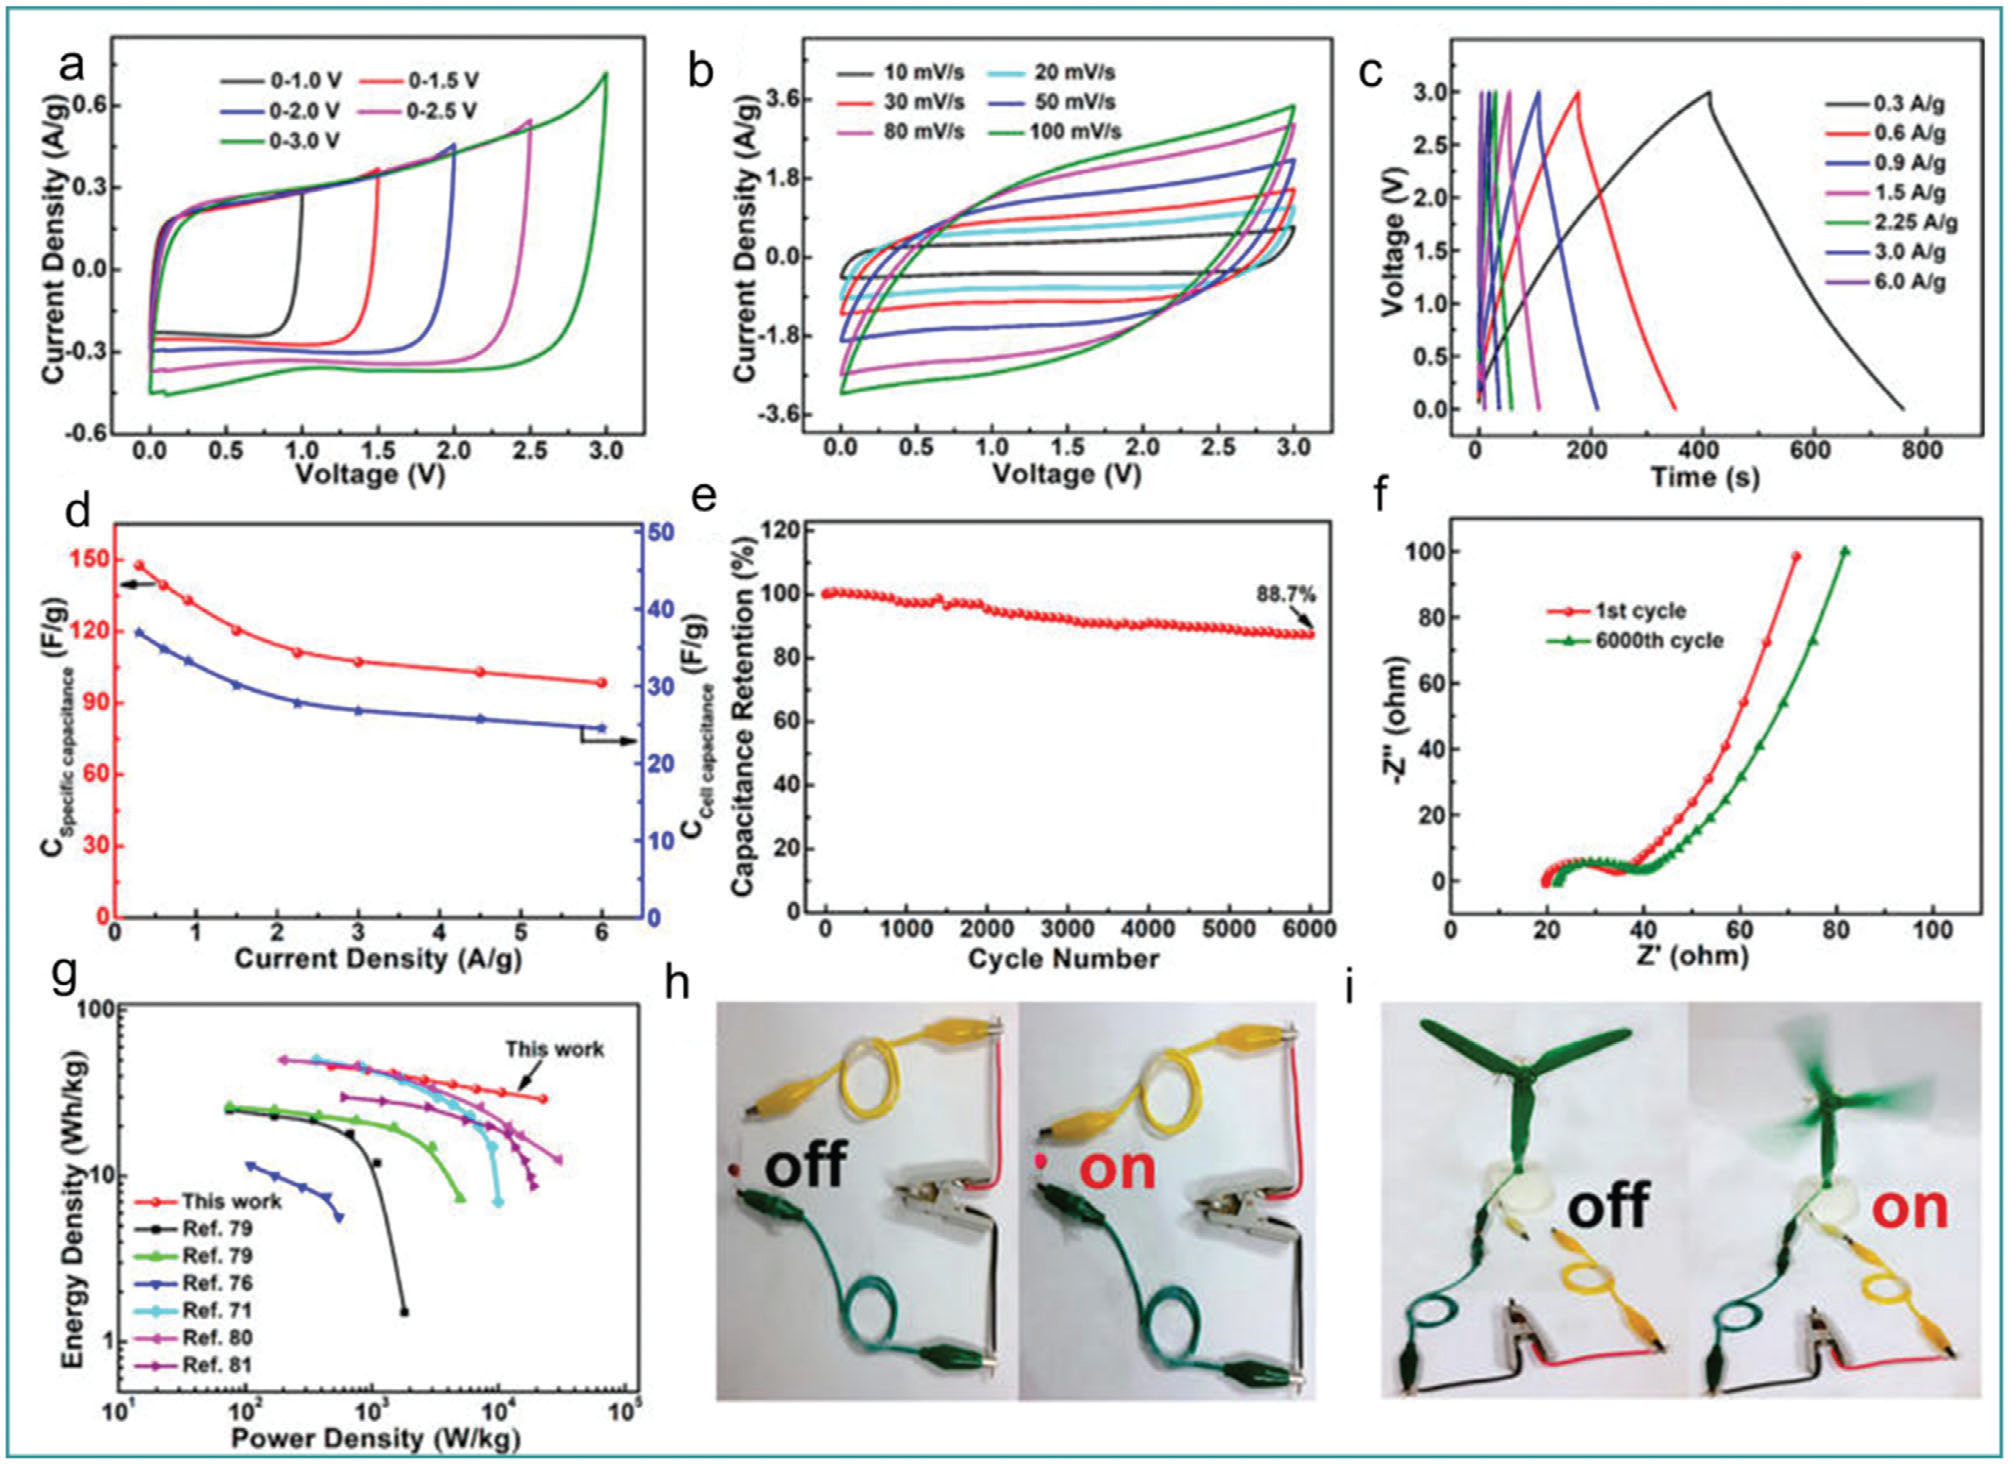
\includegraphics[width=0.7\linewidth]{electricalproperties.png}
    \caption{خواص الکتروشیمیایی ابرخازن مبتنی بر صفحه آماده شده الف) منحنی های ولتامتری چرخه ای که تحت ولتاژهای مختلف به دست می آیند. ب) منحنی های ولتامتری چرخه ای که تحت نرخ‌های مختلف اسکن جمع آوری شده اند. ج) منحنی‌های GCD تحت چگالی جریان های مختلف آزمایش شده اند. د) ظرفیت سلولی مربوطه (منحنی آبی) و ظرفیت خازنی ویژه (منحنی قرمز) تحت چگالی جریان های مختلف. ه) پایداری تناوبی برای 6000 سیکل (سرعت اسکن: $50 mV s^{-1}$ و)  نایکیست در ابتدا و انتهای 6000 سیکل جمع آوری شد. ز) نمودار راگون در مایع یونی. باتری آماده شده می تواند به عنوان منبع تغذیه برای نور ح) و فن استفاده شود.}
    \label{fig:electricalproperties}
\end{figure*}

۱) \textbf{پنجره ولتاژ بزرگ و پایدار:} همانطور که در شکل \ref{fig:electricalproperties}.الف) نشان داده شده است، ابرخازن مونتاژ شده با \gls{Borophene} لایه برداری شده با \gls{DMF} تا 3.0 ولت پنجره ولتاژ را نشان می دهد. علاوه بر این، شکل \ref{fig:electricalproperties}.ب) نشان می دهد که حتی در اسکن سریع $100 mV\; s^{-1}$، تمام منحنی های ولتامتری حلقوی شکلی تقریبا مستطیلی را نشان می دهند، \cite{luHTiO2MnO2HTiO22013} که نشان دهنده خاصیت شارژ/دشارژ سریع و رفتار خازنی نسبتاً خوبی است (شکل \ref{fig:electricalproperties}.ج) 

۲) \textbf{ظرفیت ویژه خوب:} در چگالی جریان $0.3 A\; g^{-1}$، حداکثر ظرفیت ویژه $147.6 F\; g^{-1}$به دست می آید (شکل \ref{fig:electricalproperties}.د). حداکثر ظرفیت ویژه بسیار بالاتر از ابرخازن مبتنی بر مواد مبتنی بر کربن و بور \gls{bulk} است\cite{liuElectrochemicalBehaviorGraphene2011, chenHighPerformanceSupercapacitors2011}.

۳) \textbf{قابلیت سرعت عالی:} چگالی جریان از $.0.3-6.0 A\; g^{-1}$، حدود 20 برابر افزایش می یابد، ظرفیت خازنی ویژه $98.3 F^{-1}$ است، و نرخ نگهداری ظرفیت $66.6٪$ است\cite{liScalableProductionFewLayer2018}.

4) \textbf{پایداری چرخه خوب:} شکل \ref{fig:electricalproperties}.ه) نشان می دهد که حفظ ظرفیت ویژه اولیه هنوز $88.7٪$ پس از 6000 چرخه با سرعت اسکن $50 mV s^{-1}$ است، \cite{liScalableProductionFewLayer2018} که برابر یا حتی بهتر از ابرخازن های مبتنی بر کربن است. ، حتی اگر پس از 6000 سیکل آزمایش شده توسط طیف سنجی امپدانس الکتروشیمیایی در شکل \ref{fig:electricalproperties}.و)، یک کاهش جزئی در ظرفیت وجود داشته باشد. 

5) \textbf{چگالی انرژی عالی: }تحت چگالی توان $478.5 W kg^{-1}$، چگالی انرژی $46.1 Wh\; kg^{-1}$ را می توان به دست آورد (شکل \ref{fig:electricalproperties}.ز)،\cite{shaoHighperformanceFlexibleAsymmetric2013} که برابر یا حتی بیشتر از ابرخازن های ساخته شده از کربن است. در کاربردهای عملی، پس از شارژ برای چند ثانیه، یک سلول سکه با موفقیت نور را روشن کرد (شکل \ref{fig:electricalproperties}.ح) یا فن را به حرکت درآورد (شکل \ref{fig:electricalproperties}.ی). بنابراین، با ویژگی‌های چگالی جرم کم، سطح ویژه بالا، رسانایی قابل‌توجه الکترونی و غیره، چشم‌انداز کاربرد نانومواد \gls{Borophene} برای فتوولتائیک‌های نسل بعدی و ذخیره انرژی بسیار امیدوارکننده است.

\subsection{باتری‌ها}
خواص فلزی بودن و وزن اتمی کم این امکان را فراهم می کند که \gls{Borophene} آند باتری‌ها باشد. مطالعات نظری نشان داده است \cite{atacaHydrogenStorageCalcium2009} که وقتی جاهای خالی شش ضلعی توخالی ذاتی در \gls{Borophene} فلزات جذب شده مانند لیتیوم و سدیم را محکم نگه می‌دارد، پایداری کل سیستم بالا می‌ماند یا حتی بهبود می‌یابد. مهمتر از آن، \gls{Borophene} هیچ مشکل کلی از نظر انبساط حجمی ، \gls{kinetics} کم آهسته، \gls{Intercalation} کم ندارد، که همگی در مواد آند رایج مانند \ce{NiCo2O4}، کربن سخت و \ce{Sn} وجود دارند.\cite{ponrouchHighCapacityHard2013, alcantaraNiCo2O4SpinelFirst2002,liuUltrasmallSnNanoparticles2015} به طور خلاصه، \gls{Borophene} دارای مزایای زیر به عنوان آند، به ویژه برای باتری‌های لیتیوم-یونی و سدیم-یونی و  همانطور که از نظر تئوری پیش بینی شده است.
\begin{figure*}
    \centering
    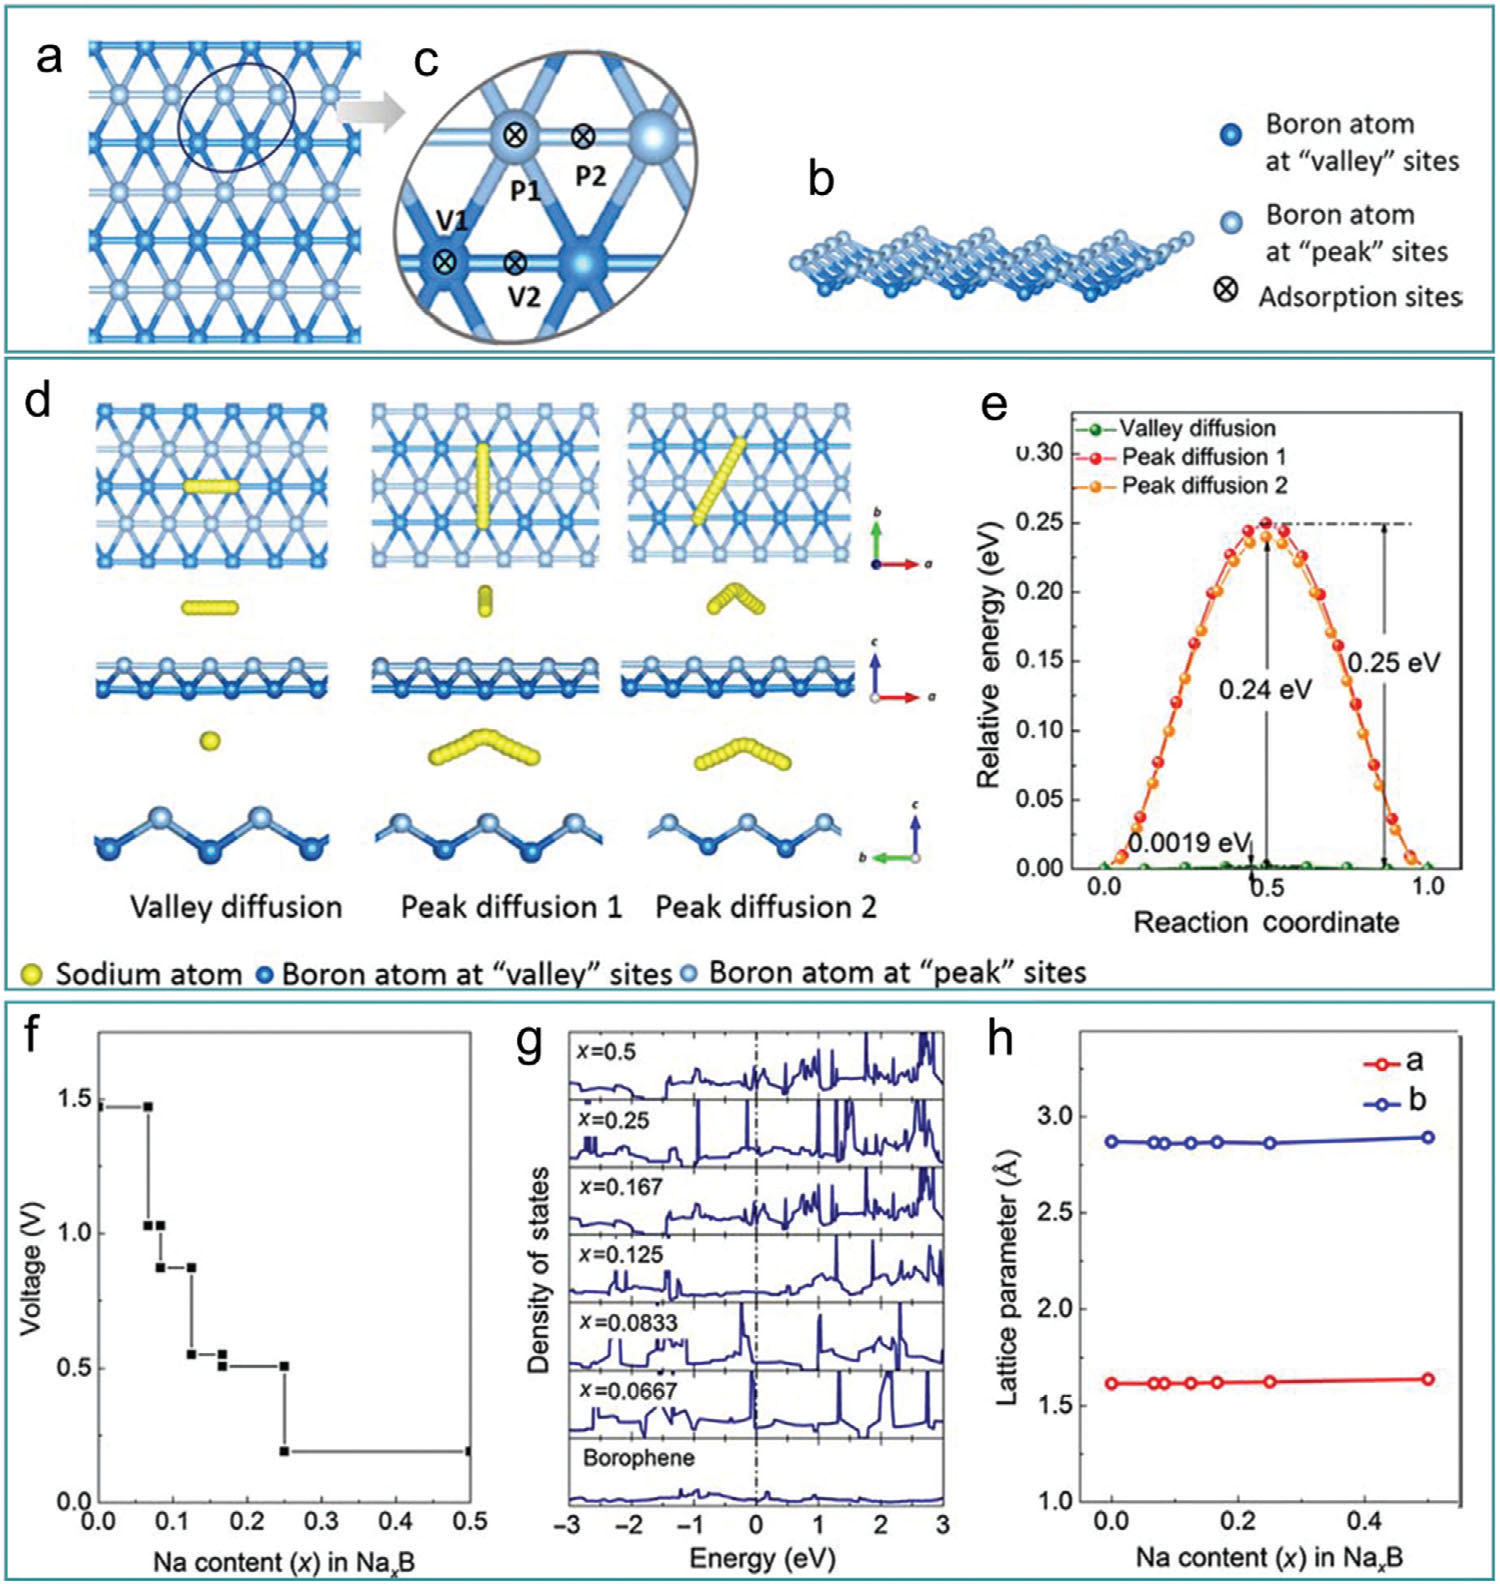
\includegraphics[width=0.7\linewidth]{absorbtion.png}
    \caption{الف) نمای بالا، ب) نمای جانبی، و ج) محل های جذب انتخابی \lr{Pmmn} بوروفین. د) سه مسیر انتشار سدیم روی بوروفین. ه) منحنی های انرژی مسیرهای انتشار. و) تغییر ولتاژ در طی فرآیند سدیاسیون. ز،ح) پارامترهای \lr{DOS} و شبکه بوروفین تحت غلظت‌های مختلف سدیم. الف – ح) با اجازه تکثیر می شود.}
    \label{fig:absorbtion}
\end{figure*}

\subsubsection{خواص رسانایی پایدار:}
\gls{Borophene} فاز \lr{Pmmn} ساختار کمانشی منحصر به فردی دارد (شکل \ref{fig:absorbtion}.الف-ج)، که در آن اتم‌های بور را می‌توان به دو گروه «قله» و «دره» با توجه به ارتفاع موقعیت‌شان تقسیم کرد.\cite{mannixSynthesisBorophenesAnisotropic2015} ساختار لایه شلی است، که می تواند پس از قرار گرفتن در غلظت‌های مختلف اتم‌های فلزی مانند سدیم و لیتیوم، انبساط حجمی کوچک (فقط ($2٪$) و تغییر شبکه را تضمین کند. بنابراین، \gls{Borophene} می‌تواند یکپارچگی ساختاری و پایداری چرخه خوبی را به عنوان ماده آند باتری نشان دهد.

\subsubsection{نرخ ظرفیت فوق العاده}
بر اساس ساختار ویژه \gls{Borophene}، \gls{Xu} و همکاران \cite{shiInitioPredictionBorophene2016} با محاسبات \gls{DFT} یک سد انرژی انتشاری بسیار کم ($0.0019\;eV$) سدیم در "جهت دره" بدست آوردند که بسیار کمتر از مواد آندی سنتی مانند \ce{Na2Ti3O7} و \ce{Na3Sb} (به ترتیب $0.19$ و $0.21\; eV$) است. بیشتر. به طور شگفت انگیزی، نرخ انتشار در آن جهت بیش از $1000$ برابر بیشتر از \ce{Na2Ti3O7} و \ce{Na3Sb} بود \cite{baggettoIntrinsicThermodynamicKinetic2013, gonzeFirstprinciplesComputationMaterial2002, panSodiumStorageTransport2013}. در نهایت، سد انرژی انتشار \ce{Li} کمی بالاتر از سدیم از طریق خواص انتشار ناهمسانگرد بود (شکل \ref{fig:absorbtion}.د،ه).  همه این مشاهدات نشان می‌دهند که \gls{Borophene} نرخ ظرفیت قابل‌توجهی به عنوان آند باتری‌های لیتیوم یا سدیم-یونی دارد، که به وضوح می‌تواند مشکل \gls{kinetics} کند را حل کند \cite{shiInitioPredictionBorophene2016}.

\subsubsection{ظرفیت نظری فوق العاده بالا:}
با در نظر گرفتن باتری های سدیم-یونی به عنوان مثال، زمانی که نسبت \ce{Na/B} (\gls{Borophene}) به $0.5$ می رسد (سدیم به طور کاملاً یکنواخت دو طرف بالا و پایین \gls{Borophene} را می پوشاند)، مقدار ظرفیت نظری به حداکثر می رسد ($1218 mAh\; g^{-1} Na_{0.5}B$)، \cite{shiInitioPredictionBorophene2016} که حداکثر مقدار و حدود سه برابر بیشتر از آند گرافیت ($372 mAh g^{-1}$) است. وضعیت حتی برای لیتیوم ($Li_{0.75}B$) به دلیل شعاع اتمی بزرگتر، که ظرفیت نظری آن $1860$ میلی آمپر ساعت بر گرم است، در حدود چهار برابر بیشتر از آند گرافیت است \cite{jiangBorophenePromisingAnode2016} بنابراین، \gls{Borophene} می‌تواند به طور قابل‌توجهی کاربرد \gls{Intercalation} فلزات را افزایش دهد، تراکم انرژی باتری و چگالی توان را افزایش دهد.

\subsubsection{:جلوگیری موثر از تشکیل دندریت}
باتری‌های لیتیوم و سدیم یونی هر دو به دلیل داشتن فلزات بسیار واکنش‌پذیر با دمای ذوب پایین، با مسائل \gls{Dendrite} به چالش کشیده می‌شوند، \cite{mortazaviElasticSofteningAlloy2013, chevrierChallengesNaionNegative2011} که یک نگرانی جدی ایمنی را نشان می‌دهد که هنوز به طور موثر حل نشده است. با این حال، \gls{Borophene} ممکن است بتواند این را معکوس کند. \gls{Xu} و همکاران \cite{shiInitioPredictionBorophene2016} دریافت که میانگین ولتاژ مدار باز محاسبه‌شده یک باتری سدیم یونی با \gls{Borophene} به عنوان ماده آند به اندازه $0.53$ ولت در هنگام شارژ کردن است و پیوند بین \gls{Borophene} و سدیم قوی است. (شکل \ref{fig:absorbtion}.و-ح). هر دو نشان می‌دهند که اتم‌های فلز به‌جای خوشه‌بندی برای تشکیل یک فاز فلزی جداگانه، به‌طور یکنواخت بوروفین را پوشانده‌اند، که می‌تواند به طور مؤثری از تشکیل دندریت جلوگیری کند و در عین حال چگالی انرژی بالایی را حفظ کند. اگرچه داده‌های بالا نشان می‌دهند که \gls{Borophene} به عنوان ماده آند باتری،  امیدوارکننده است، تحقیقات فعلی کاملاً تئوری باقی مانده است و آزمایش‌های وسیعی برای تأیید کاربردهای عملی آن هنوز مورد نیاز است.
\begin{figure*}
    \centering
    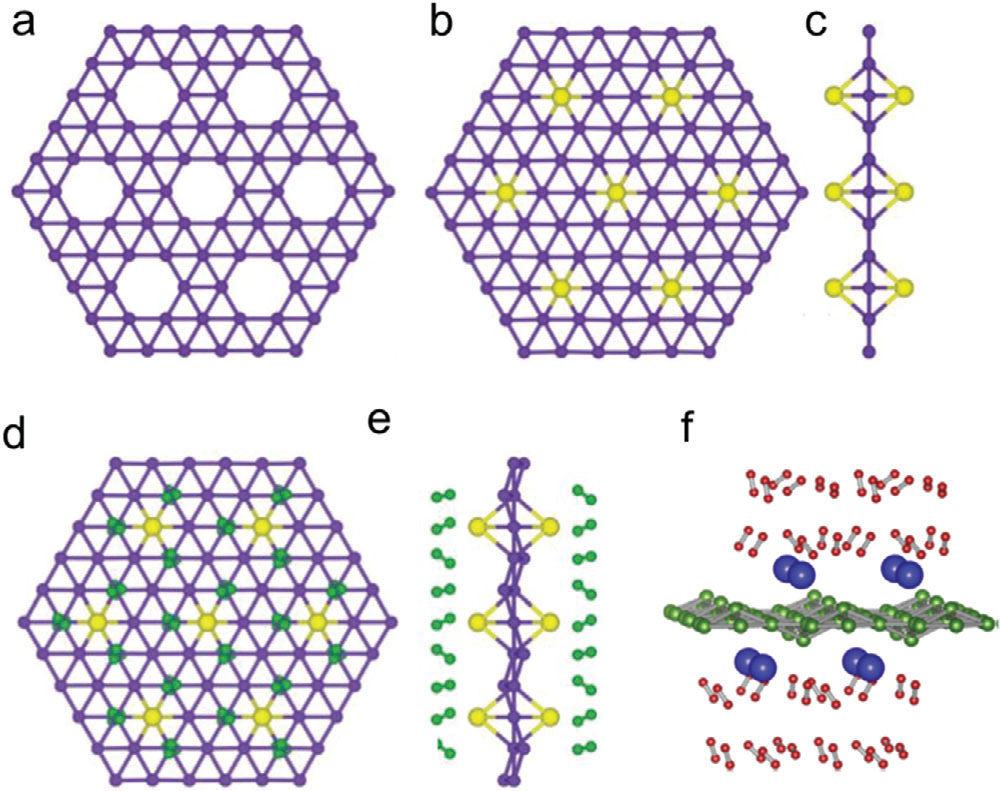
\includegraphics[width=0.7\linewidth]{alphasheet.png}
    \caption{الف) ساختار بوروفین صفحه $\alpha$ بدون لیتیوم. ب، ج) ساختار بهینه شده بوروفین صفحه $\alpha$ با اتم های لیتیوم (کره های زرد). د، ه) ساختار بهینه شده بوروفین $\alpha$-صفحه با لیتیوم پس از جذب \ce{H2}. الف-ه) ساختار بهینه‌شده بوروفین با تزئین کلسیم (کره‌های آبی) پس از جذب \ce{H2}}
    \label{fig:alphasheet}
\end{figure*}

\subsection{ذخیره سازی هیدروژن}
با توجه به سوخت محدود و مسائل زیست محیطی، توسعه یک ماده مناسب برای ذخیره سازی هیدروژن ضروری است. برای ارزیابی توانایی ذخیره هیدروژن یک ماده، دو شاخص، یعنی انرژی جذب و ظرفیت جذب \ce{H2} مورد نیاز است. با توجه به انرژی جذب، انرژی جذب در محدوده $0.2-0.6\; eV$ لازم است تا اطمینان حاصل شود که مولکول های \ce{H2} می توانند به طور پایدار و آسان روی سطح مواد جذب شوند. با توجه به ظرفیت جذب \ce{H2}، هدف تعیین شده توسط وزارت انرژی ایالات متحده 7.5 درصد وزنی است. اخیراً مشخص شده است که \gls{Borophene} به دلیل وزن سبک و مساحت سطح ویژه بزرگ، کاندیدای ذخیره‌سازی \ce{H2} است، به ویژه هنگامی که گرافین یا فلزات واسطه اضافه می‌شوند. مطالعات قبلی انرژی جذب \ce{H2} را بر روی سطح بوروفن خالص تجزیه و تحلیل کرده و دریافتند که حداکثر آن کمتر از $0.01\; eV$ است که برای ذخیره عملی \ce{H2} بسیار کوچک است.
خوشبختانه، با کمک فلزات قلیایی یا واسطه، می توان فعالیت شیمیایی را افزایش داد و برهمکنش بین \gls{Borophene} و \ce{H2} را تقویت کرد. در طول جذب \ce{H2}، \gls{Borophene} نیازی به ایجاد نقص برای جذب فلزات ندارد، زیرا \glsdesc{HH} های آن می توانند به عنوان مکان های جذب فلز استفاده شوند (شکل \ref{fig:alphasheet}.آ-ج) \cite{shangTwoDimensionalBoron2018} \gls{Tang} و همکاران \cite{tangTheoreticalInvestigationCalcium2018} دریافتند که فاز $\beta_{12}$ \gls{Borophene} با تزئینات کلسیم کاندیدای مناسبی برای ذخیره سازی \ce{H2} است. \gls{Borophene} فاز $\beta_{12}$ به طور طبیعی می تواند \glsdesc{HH} ها را تشکیل دهد و به کلسیم محل جذب خوبی می دهد (شکل \ref{fig:alphasheet}.f) \cite{wangCadecoratedNovelBoron2016} ظرفیت جذب \ce{H2} حدود $8.92$ درصد وزنی است. برای $\chi_3$ فاز \gls{Borophene} با کلسیم؛ همچنین می‌تواند به ظرفیت جذب \ce{H2} 7.2 \lr{wt٪}، نزدیک به گرافین دست یابد. برای مثال، \gls{Borophene} $\beta_{12}$ فاز دارای لیتیوم می تواند به ظرفیت جذب \ce{H2} $10.85$ درصد وزنی دست یابد \cite{liuLiDecorated12BorophenePotential2017} و صفحه تزئین شده با لیتیوم می تواند حداکثر $10.75$ درصد وزنی \ce{H2} را جذب کند که نشان دهنده جذب حداکثر 3 مولکول \ce{H2} است. برای هر اتم لی (شکل \ref{fig:alphasheet}.d,e).\cite{erDFTStudyPlanar2009} علاوه بر این، \gls{Borophene} مثلثی کمانش شده با لیتیوم، ظرفیت جذب \ce{H2} $13.7$ درصد وزنی است.\cite{shangTwoDimensionalBoron2018, liHighHydrogenStorage2017} علاوه بر این، \gls{Borophene} تزئین شده با لیتیوم $(\nu= 1/8)$ با ظرفیت ذخیره سازی \ce{H2} $15.2$6 درصد گزارش شده است \cite{liUltrahighCapacityMolecularHydrogen2015}.

\begin{figure*}
    \centering
    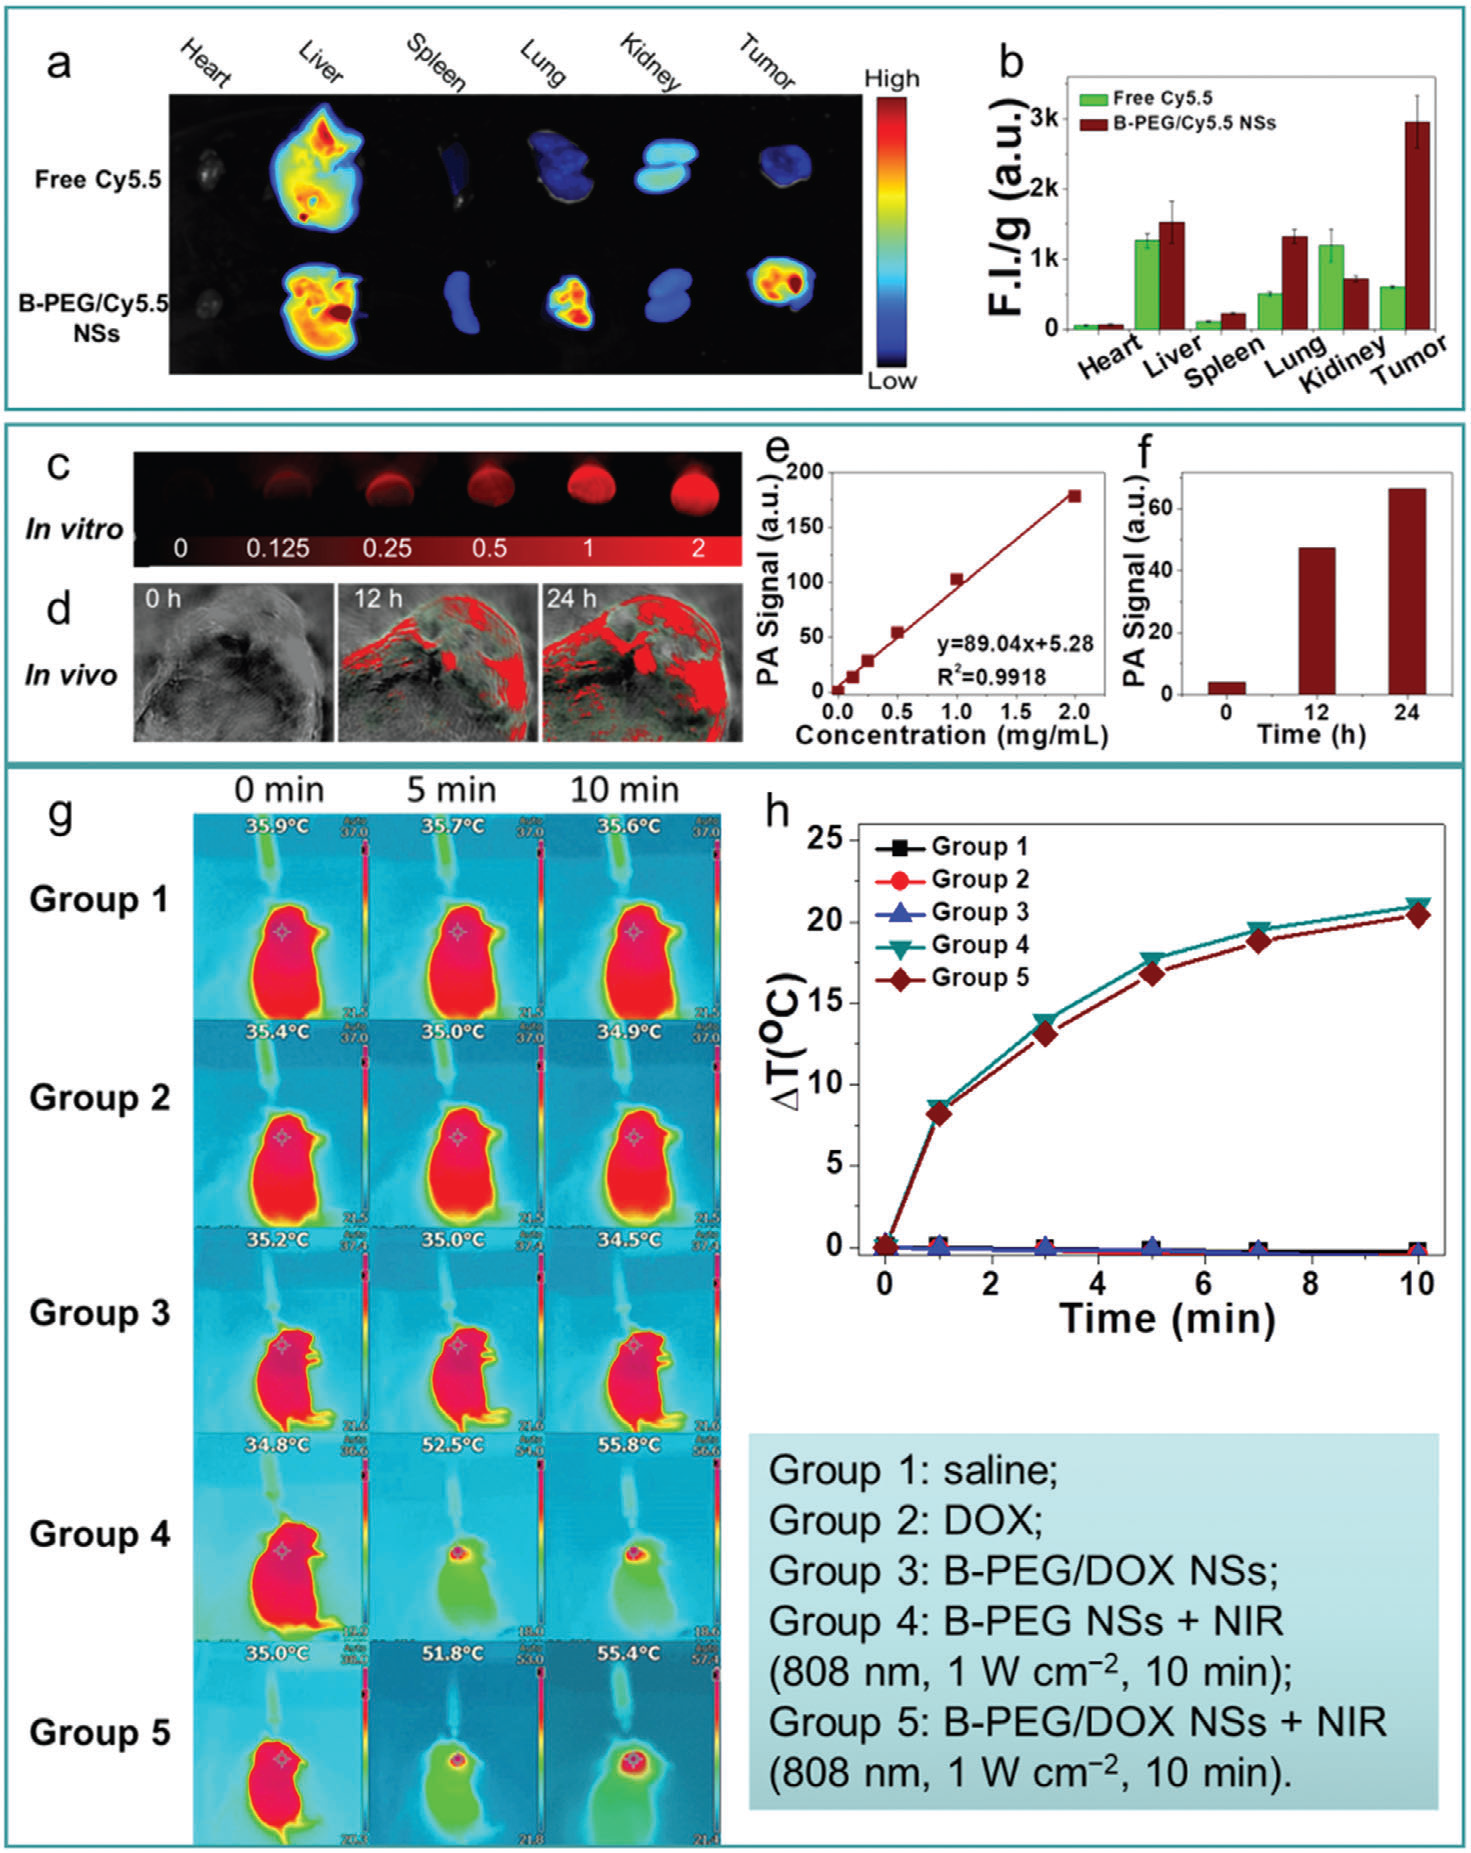
\includegraphics[width=0.9\linewidth]{Multimodal.png}
    \caption{تصویربرداری چندوجهی از NS های مبتنی بر . الف) تشخیص اندام‌ها و تومورهای اصلی با تصویربرداری \gls{fluorescence}. ب) توزیع زیستی نیمه کمی اندام های اصلی و تومورها. ج) تصاویر \lr{PA} از \lr{B-PEG NSs} با غلظت های مختلف ($0$،$ 0.125$،$ 0.25$، $0.5$، $0.1$، و $0.2$ میلی گرم بر لیتر) در داخل بدن. د) تصاویر تومور \lr{PA}. ه) رابطه خطی بین مقادیر \lr{PA} و غلظت \lr{B-PEG NSs}. و) تجزیه و تحلیل کمی مقادیر \lr{PA}. ز) تصاویر فتوترمال و ح) مشخصات دمایی موش‌ها.)}
    \label{fig:Multimodal}
\end{figure*}

\subsection{تصویربرداری زیستی}
تصویربرداری زیستی، از جمله تصویربرداری \gls{fluorescence}، \cite{gaoVivoCancerTargeting2004, medintzQuantumDotBioconjugates2005} تصویربرداری \gls{photothermal}، \cite{huangCancerCellImaging2006} و تصویربرداری \gls{photoacoustic} (\gls{PA})، \cite{beardBiomedicalPhotoacousticImaging2011} می‌تواند مکان و اندازه تومورها را فراهم کند و یک فناوری مهم برای تشخیص بالینی و درمان تومورها است. اطلاعات ضایعه نمایش داده شده توسط هر حالت تصویربرداری متفاوت است و هر حالت تصویربرداری مزایا و معایب خاص خود را دارد. بنابراین، اطلاعات تومور را می توان به طور جامع تری از طریق یک پلتفرم تصویربرداری چندوجهی تومور ارائه کرد، که می تواند تا حد زیادی خطر تشخیص اشتباه را کاهش دهد. \gls{Ji} و همکاران \cite{jiNovelTopDownSynthesis2018} یک پلتفرم تصویربرداری چندوجهی تومور مبتنی بر \gls{Borophene} ساخته شد که می تواند به طور همزمان تصویربرداری \gls{fluorescence}، تصویربرداری \lr{PA} و تصویربرداری \gls{photothermal} را انجام دهد. مواد فلورسنت بر روی حامل بارگذاری می شود و فرمولاسیون در تومور با روش های هدف گیری فعال یا هدف گیری غیرفعال غنی می شود. عکس تصویربرداری \gls{fluorescence} از موش توموری که \gls{Borophene} نشاندار \lr{Cy 5.5} اصلاح شده توسط \gls{PEG} (\gls{B-PEG NS} با نشاندار \lr{Cy5.5}) تزریق شده است (شکل \ref{fig:Multimodal}.الف،ب) به وضوح بین تومورهای بدخیم و بافت‌های طبیعی تمایز قائل شد. در مقایسه  فلورسنت بدون رنگ \lr{Cy5.5}، \gls{B-PEG NS} با نشاندار \lr{Cy5.5} به دلیل اثر \gls{EPR}، زمان گردش خون طولانی‌تر و تجمع تومور بهتری دارد. علاوه بر این، \gls{B-PEG NS}نیز یک عامل بالقوه \gls{PA} است. تصویربرداری \gls{PA} یک روش تصویربرداری زیستی غیر مخرب است که از \gls{ultrasound} به عنوان واسطه استفاده می کند. در مقایسه با تصویربرداری نوری و تصویربرداری صوتی، تصویربرداری \gls{PA} بر بسیاری از کاستی‌های این دو فناوری تصویربرداری غلبه کرده و عمق کاوش، کنتراست تصویر و وضوح فضایی را افزایش می‌دهد. تصویربرداری \gls{PA} می‌تواند نمودار ساختار تومور موش تومور را در زمان‌های مختلف پس از تزریق \lr{B-PEG NS} نشان دهد (شکل \ref{fig:Multimodal}.د،ه)، و شدت سیگنال \lr{PA} با غلظت \lr{B-PEG NS} همبستگی مثبت دارد (شکل \ref{fig:Multimodal}.ه) - هر چه غلظت \lr{B-PEG NS} بیشتر باشد، سیگنال قوی تر است. نتایج فوق نشان داد که \lr{B-PEG NS} می تواند به طور موثر در محل های تومور غنی شود و یک عامل بالقوه \gls{PA} است. علاوه بر این، \gls{Borophene} دارای نرخ تبدیل \gls{photothermal} و پایداری \gls{photothermal} خوبی است و انرژی نور را به انرژی گرمایی تحت تابش نور مادون قرمز نزدیک (\gls{NIR}) تبدیل می‌کند. توزیع \gls{Borophene} و تغییرات دما در اندام های مختلف را می توان با دوربین گرمایی مادون قرمز نیز بدست آورد. به عنوان مثال، در یک آزمایش، موش‌ها به پنج گروه تقسیم شدند، گروه‌های چهار و پنج پس از تزریق داخل وریدی \lr{B-PEG NSs} یا \lr{B-PEG/DOXNSs} (دوکسوروبیسین بارگذاری شده با \lr{B-PEG NSs}) و درجه حرارت در تومور این دو گروه از 308 به 328 کلوین افزایش یافت، در حالی که دمای سایر گروه‌ها بدون \gls{B-PEG NS} یا \gls{NIR} در \lr{≈308K} ثابت ماند (شکل \ref{fig:Multimodal}.و،ز). در نتیجه، \gls{Borophene} را می توان به طور بالقوه در پلت فرم های تصویربرداری زیستی چندوجهی تومور مورد استفاده قرار داد و به دستیابی به تشخیص دقیق و درمان دقیق تومورها کمک کرد.

\begin{figure*}
    \centering
    \includegraphics[width=0.8\linewidth]{UV.png}
    \caption{الف) طیف \lr{UV B-PEG NSs}. ب) مشخصات تغییر دما \lr{B-PEG NSs} تحت لیزر 808 نانومتر. ج) رابطه خطی بین $\ln\theta$ و زمان. د) مشخصات گرمایش \lr{B-PEG NSs} پس از پنج سیکل. ه) اسکن تصاویر میکروسکوپ الکترونی عبوری–EDS از \lr{B-PEG/DOX NSs}. و) طیف UV بارگیری بوروفین با DOX. ز) توانایی بوروفین برای بارگیری داروهای شیمی درمانی. ح) منحنی های DOX را تحت pH های مختلف آزاد کنید. ی-ن) آزمایشات سلولی. ی) ارزیابی ایمنی بوروفین در سلول های مختلف (بدون لیزر). ک) ارزیابی سمیت بوروفین در سلول های مختلف (لیزر 808 نانومتر). ل) زنده ماندن نسبی سلول های تومور تحت درمان های مختلف. م) تصاویر CLSM از سلول های تومور رنگ شده با PI (مرده، قرمز) و AM (زنده، سبز). ن) عکسهای دیجیتالی موشها و تومورهای معرف در گروههای مختلف تحت درمان به مدت 14 روز. ن) وزن بدن موش‌ها. G1: کنترل؛ G2: داروهای شیمی درمانی. G3: بوروفین + داروهای شیمی درمانی. G 4: بوروفین + لیزر 808 نانومتری. G5: بوروفین} + داروهای شیمی درمانی + لیزر 808 نانومتری.
    \label{fig:UV}
\end{figure*}

\subsection{تحویل دارو }
انتشار موضعی داروهای شیمی درمانی کلید کاهش عوارض جانبی شیمی درمانی است. بنابراین، طراحی یک پلتفرم آزادسازی دارو با پاسخ ریزمحیط تومور هوشمند بسیار مهم است. سطح ویژه بسیار بالا \gls{Borophene} فضایی را برای بارگیری دارو و نقاط لنگر برای اصلاح گروه عملکردی فراهم می کند و آن را به ماده‌ای مناسب برای بسیاری از جنبه‌های درمان ضد سرطان تبدیل می‌کند. در یک سیستم دارورسانی مبتنی بر \gls{Borophene}، دوکسوروبیسین (\gls{DOX}) با \gls{Borophene} انکوبه شد (نرخ بارگذاری: \lr{114\%}) و سیستم با \lr{PEG-NH2} پوشانده شد تا به گردش طولانی مدت داروهای شیمی درمانی در بدن دست یابد (شکل \ref{fig:UV}د-ز). ) اصلاح موفقیت آمیز \lr{PEG} و بارگذاری \gls{DOX} را نشان داد.\cite{jiNovelTopDownSynthesis2018} به عنوان یک حامل دارو، \gls{Borophene} \gls{pH} و واکنش گرمایی خوبی نشان داد. در \gls{pH} 7.4 و 5.0، نرخ آزادسازی \gls{DOX} توسط \gls{Borophene} به ترتیب \lr{8.3٪} و \lr{24٪} بود (شکل \ref{fig:UV}.ح). \gls{pH} ریزمحیط تومور کمتر از بافت طبیعی است (ادبیات)، که به \gls{Borophene} اجازه می دهد تا به رهاسازی هدفمند دارو در تومور دست یابد. علاوه بر این، \gls{Borophene} همچنین حامل دارو برای پاسخ \gls{NIR} است. تحت شرایط فوق، 5 دقیقه نور \gls{NIR} برای گروه‌های \gls{pH} مختلف اعمال شد، با سرعت انتشار دارو در \gls{pH} 7.4 به \lr{41.4٪} و در \gls{pH} 5.0 افزایش به \lr{77.6٪} (شکل \ref{fig:UV}.ح). به طور خلاصه، \gls{Borophene} با ظرفیت بارگیری دارو بالا و \gls{pH} و پاسخ دوگانه مادون قرمز، یک پلت فرم یکپارچه دارورسانی امیدوارکننده برای تشخیص و درمان سرطان است.

\subsection{درمان سرطان}
\gls{photothermal} می‌تواند به درمان غیر تهاجمی کم تهاجمی سرطان دست یابد. این روش از تشعشعات \gls{NIR} برای تابش بافت تومور استفاده می کند و دمای بافت تومور به دلیل تبدیل \gls{photothermal} افزایش می‌یابد و منجر به مرگ سلول‌های تومور می‌شود.\cite{prasadMechanismCellDeath2007} یک عامل درمانی \gls{photothermal} ایده‌آل باید سمیت کم، جذب نور قوی، راندمان تبدیل \gls{photothermal} بالا و پایداری \gls{photothermal} در پنجره \lr{NIR} (650-950 نانومتر) داشته باشد.\cite{jangGoldNanorodPhotosensitizerComplex2011, chengPEGylatedWS2Nanosheets2014} \gls{Ji} و همکاران \cite{jiNovelTopDownSynthesis2018} از \gls{Borophene} در درمان \gls{photothermal} تومورها استفاده کرد و به اثرات درمانی خوبی دست یافت. سه معیار مهم برای یک عامل \gls{photothermal} عالی عبارتند از: راندمان تبدیل \gls{photothermal}، پایداری \gls{photothermal} و جذب \lr{UV}. این خواص \gls{Borophene} مورد ارزیابی قرار گرفت. جذب \lr{UV-vis-NIR} \gls{Borophene} بالا است (شکل \ref{fig:UV}.الف). \gls{Borophene} در یک محلول آبی پراکنده شد و با نور مادون قرمز 808 نانومتری \lr{(2 $W\; cm^{-2}$)} به مدت 5 دقیقه تحت تابش قرار گرفت و تغییرات دمایی \gls{Borophene} در غلظت‌های مختلف ثبت شد (شکل \ref{fig:UV}.ب). با توجه به نتایج، تحت شرایط فوق، بالاترین دمای انتقال (\lr{310 K}) در غلظت 0.2 میلی گرم در میلی لیتر در لیتر به دست آمد. در مقایسه با سایر عوامل \gls{photothermal} گزارش شده، مانند نقاط کوانتومی فسفر سیاه \lr{(28.4\%)} و نانومیله های طلا (\lr{21\%})، \gls{Borophene} دارای راندمان تبدیل \gls{photothermal} بالاتری \lr{(42.5\%)} است (شکل \ref{fig:UV}.ج). علاوه بر این، پایداری \gls{Borophene} با تابش مکرر \gls{NIR} ارزیابی شد. پس از پنج دور تابش و خنک‌سازی مکرر، ویژگی‌های \gls{photothermal} نانوصفحات به سختی تغییر کرد، که نشان می‌دهد پایداری نور گرمایی خوبی دارد (شکل \ref{fig:UV}.د). اثربخشی و زیست سازگاری بالا شاخص های مهمی برای ارزیابی اینکه آیا یک ماده می تواند با موفقیت در زمینه زیست پزشکی استفاده شود یا خیر است. بنابراین، سمیت سلولی و در دسترس بودن \gls{photothermal} \gls{Borophene} هم در شرایط آزمایشگاهی و هم در داخل بدن ارزیابی شده است. غلظت های مختلف \gls{Borophene} با چهار نوع سلول سرطانی به مدت 48 ساعت انکوبه شد و زنده ماندن سلول مورد بررسی قرار گرفت. سمیت سلولی ناچیز مشاهده شد (شکل\ref{fig:UV}) که نشان می دهد \gls{Borophene} زیست سازگاری خوبی دارد. بر این اساس، \gls{Borophene} به عنوان یک عامل \gls{photothermal} برای ارزیابی اثر ضد توموری یک سیستم دارورسانی مبتنی بر بور استفاده شد (شکل \ref{fig:UV}.ک-ل). در غلظت \lr{B-PEG NSs} 200 میکروگرم $mL^{-1}$ و تحت نور \gls{NIR}، بیش از 80 درصد از سلول های تومور \lr{MCF7} مردند و تقریبا 90 درصد از سلول های تومور \lr{PC3} مردند. علاوه بر این، به دنبال تزریق داخل وریدی \lr{B-PGE/DOX} و تابش محل تومور با نور مادون قرمز، حجم تومور در موش‌ها به طور قابل توجهی کاهش یافت و وزن بدن موش به سختی تحت تاثیر قرار گرفت (شکل \ref{fig:UV}.م،ن). به طور خلاصه، \gls{Borophene} یک پلت فرم عالی درمان ضد تومور با راندمان تبدیل \gls{photothermal} بالا \lr{(42.5٪)}، پایداری گرمایی بالا، توانایی حذف تومور با راندمان بالا، و زیست سازگاری خوب است.

\subsection{حسگرهای زیستی}
حسگرهای زیستی می‌توانند به سرعت و با دقت بیومارکرهایی مانند هورمون‌ها، پروتئین‌ها و گلوکز را با ویژگی و حساسیت بالا شناسایی کنند، \cite{taoEmergingTwodimensionalMonoelemental2019} و برای تشخیص نمونه خون، تشخیص زودهنگام سرطان و آنالیز بالینی در دسترس هستند و توجه زیادی را در زمینه زیست‌پزشکی به خود جلب می‌کنند. نانومواد دوبعدی به دلیل عملکرد الکتروشیمیایی برتر، نسبت سطح به حجم بالا،\cite{huangAdsorptionGasMolecules2018} مکان‌های فعال‌تر سطح، \cite{ranjanBoropheneNewSensation2020, li2DBoronSheets2020} و تحرک‌های الکترونی بالا در ضخامت‌های تک لایه، کاندیدای عالی برای حسگرهای زیستی شده‌اند \cite{liRatiometricImmunoassaysBuilt2019, ranjanBoropheneNewSensation2020} \gls{Borophene} پتانسیل کاربرد بیوسنینگ وسیعی را برای تشخیص گاز نشان می‌دهد زیرا سطح فوق‌العاده‌ای دارد و قابلیت جذب عالی برای مولکول‌های گاز دارد \cite{li2DBoronSheets2020} به عنوان حسگر زیستی، نه تنها می تواند گازهای غیر سمی مانند اتانول (\ce{CH2OH}) \cite{xieTwoDimensionalBoropheneProperties2020} و آمونیاک \ce{(NH3)}، \cite{huangAdsorptionGasMolecules2018}، بلکه گازهای بسیار سمی مانند فرمالدئید (\ce{CHOH})، \ce{CO}، و \ce{NO} \cite{huangAdsorptionGasMolecules2018} را نیز کنترل کند. حتی نمی‌توان آن را با حسگرهای زیستی گاز گرافین و فسفرن، که هر دوی آنها اخیراً به عنوان حسگرهای زیستی بسیار حساس در نظر گرفته شده‌اند، پایش کرد. علاوه بر قدرت جذب نسبتاً قوی گازهای بسیار سمی روی سطح \gls{Borophene}، دلیل اینکه \gls{Borophene} برای بیوسنسورهای گازی بسیار سمی مناسب‌تر است، تا حدی توسط باند گپ الکترونی فعال می‌شود که سایر مواد دو بعدی مانند گرافین فاقد آن هستند. شکاف باند الکترونی \gls{Borophene} می تواند به سرعت کاهش یابد زمانی که گاز جذب می شود، انتقال الکترون های زیادی را تسهیل می کند و هدایت الکتریکی را افزایش می دهد، و بنابراین، \gls{Borophene} را در کاربردهای حسگرهای زیستی گاز بسیار سمی قابل توجه می کند. \cite{shuklaRealization2DBorophene2017} \ce{HCOH} به عنوان ماده سرطان‌زای بسیار سمی و تحریک‌کننده شناخته می‌شود و قرار گرفتن در معرض آن ممکن است باعث واکنش‌های نامطلوب مانند آبریزش چشم، تحریک تنفسی و آسم شود. به واکنش شیمیایی عالی و پایداری گرمایی بالا \cite{cockcroftOCCUPATIONALASTHMACAUSED1982} بنابراین، لازم است یک بیوسنسور \ce{HCOH} با حساسیت بالا ایجاد شود تا به طور موثر از اثرات نامطلوبی که \ce{HCOH} ممکن است منجر شود، جلوگیری شود. انصاری و همکاران \cite{kootenaeiB36BoropheneElectronic2016} پتانسیل کاربرد \ce{B36} را به عنوان حسگر زیستی \ce{HCOH} با تجزیه و تحلیل ساختار توخالی شش ضلعی تلفیقی آن با محاسبات \gls{DFT} مورد مطالعه قرار دادند و دریافتند که حضور \ce{HCOH} می تواند به طور قابل توجهی رسانایی \ce{B36} را افزایش دهد و در نتیجه سیگنال های الکتریکی تولید کند. علاوه بر این، قدرت سیگنال‌های الکتریکی می‌تواند همراه با مولکول‌های جذب‌شده \ce{HCOH} افزایش یابد، که نشان می‌دهد \ce{B36} حساسیت بالایی به غلظت (یا فشار) \ce{HCOH} دارد و به عنوان حسگر زیستی \ce{HCOH} چشم‌انداز زیادی خواهد داشت. از نقطه نظر کاربرد عملی، این همچنین نشان می دهد که \gls{Borophene} ممکن است در تشخیص غلظت برخی از گازهای سمی برجسته تر باشد. هوانگ و همکاران \cite{huangAdsorptionGasMolecules2018} ویژگی‌های انتقال \gls{Borophene} را پس از جذب گاز \ce{CO} و \ce{NO} به ترتیب با استفاده از روش‌های مبتنی بر \gls{NEGF} تجزیه و تحلیل کرده‌اند. مشخص شد که انرژی جذب بسیار زیاد است و در نتیجه مقادیر زیادی بار روی سطح \gls{Borophene} انتقال می‌یابد که نشان می‌دهد \gls{Borophene} کاندیدای عالی برای حسگرهای زیستی جدید گاز است. \ce{CO} و \ce{NO} چشم انداز خوبی در ضد التهاب، ضد باکتری، ضد تومور و غیره نشان داده اند \cite{otterbeinCarbonMonoxideHas2000} با این حال، عوامل کنترل نشده زیادی در حمل و نقل گاز وجود دارد، مانند کنترل دوز و تحویل هدفمند. بنابراین، رهاسازی ایمن و قابل کنترل و نظارت بر غلظت در زمان واقعی در داخل بدن، کلیدهایی برای تسهیل تحول بالینی بیشتر گاز درمانی \ce{CO} و \ce{NO} هستند. اکنون که حسگرهای زیستی \gls{Borophene} به تغییر غلظت \ce{CO} و \ce{NO} حساس هستند، می توان آنها را برای نظارت موثر بر غلظت گاز در گاز درمانی \ce{CO} و \ce{NO} در تحقیقات آینده در نظر گرفت. بعلاوه، بیوسنسور هیبریدی متشکل از پلیمرهای مبتنی بر \gls{Borophene} و هیدروژل که در پزشکی احیا کننده به عنوان داربست چسب استفاده شده است، به جرأت در نظر گرفته شده و به عنوان یک دستگاه هوشمند و بسیار حساس در نظر گرفته شده است که می تواند \gls{pH}، دما و سایر محرک‌ها را به نوری تبدیل کند. ، سیگنال های الکتریکی و مکانیکی. این حسگر زیستی قرار است در زمینه های زیست پزشکی مانند آزمایش خون استفاده شود \cite{inchingoloNonsyndromicMultipleSupernumerary2010} اگرچه حسگر زیستی \gls{Borophene} از نظر تئوری یک دستگاه متمایز است، به ویژه برای تشخیص گاز، کاهش پایداری پس از جذب گاز و قابلیت استفاده مجدد کم به دلیل انرژی های جذب بالا، هر دو مسائل مهمی هستند که باید مورد توجه قرار گیرند. از این رو، برای تحقق تبدیل حسگرهای زیستی \gls{Borophene} در زمینه زیست پزشکی، تحقیقات جامع تری برای روشن شدن اثرات سیتوتوکسیک، پایداری طولانی مدت، اثرات هنگام تماس نزدیک با بافت های بیولوژیکی و غیره مورد نیاز است.\cite{tatulloBorophenePromising2D2019} علاوه بر این، \gls{Borophene} هنگام قرار گرفتن در معرض هوا ناپایدار است. بنابراین، لازم است واکنش‌های خارجی احتمالی، مانند واکنش‌ها با وسایل فلزی \cite{inchingoloOralPiercingOral2011} یا متابولیت‌های سیگار کشیدن، در نظر گرفته شود \cite{tatulloCrosstalkOralGeneral2016}.

% \section{چشم انداز}
% \subsection{کاربردهای بالقوه بوروفینین در زمینه زیست پزشکی} انتظار می‌رود که \gls{Borophene} در بسیاری از کاربردهای جالب در زیست‌پزشکی، علاوه بر درمان نوری، دارورسانی، تصویربرداری چندوجهی تومور و سایر عملکردها مورد استفاده قرار گیرد. واکسن‌های تومور در سال‌های اخیر مرکز توجه بوده‌اند.\cite{rosenbergCancerImmunotherapyMoving2004, nestleVaccinationMelanomaPatients1998}[240,241] در مقایسه با شیمی‌درمانی و رادیوتراپی، عوارض جانبی آن‌ها کوچک‌تر است و می‌توانند با فعال کردن سیستم ایمنی بدن خود از رشد، گسترش و عود تومور جلوگیری کنند.\cite{hirschowitzImmunotherapyLungCancer2009}[242] با این حال، واکسن های تومور در حال حاضر توسعه یافته مشکلاتی مانند مشکل در جمع آوری سلول های مرتبط با ایمنی، تحویل آنتی ژن ناکارآمد، یا توانایی ضعیف کشتن تومور دارند. \cite{dunnCancerImmunoeditingImmunosurveillance2002, chenElementsCancerImmunity2017, gibneyPredictiveBiomarkersCheckpoint2016}[243-245] \lr{Ma et al.} یک پلت فرم تحویل واکسن تومور "یکی برای همه" ایجاد کرده اند که با استفاده از گرافین اکسید شده (مواد دوبعدی) به عنوان یک شاسی، جذب/فعال سازی سلول های ارائه دهنده آنتی ژن \lr{(APC)}، تحویل آنتی ژن و ارائه متقابل را برای حل مشکلات موجود واکسن های تومور ادغام می کند. . در مقایسه با نانوحامل‌های کروی \ch{0D}، گرافین اکسید شده دوبعدی می‌تواند \lr{APC} ‌هاو متعاقب آن آنتی ژن را به طور موثرتری ارتقا دهد و به عنوان یک سیتوکین و مخزن آنتی ژن مرتبط با ایمنی نقش داشته باشد. مشاهدات تجربی نشان می دهد که وقتی گرافین اکسید شده وارد ماکروفاژها می شود، آنتی ژن را تا می کند و هوشمندانه در چین و چروک‌ها می پیچد تا از آنتی ژن در برابر آنزیم های موجود در پاکت محافظت کند. علاوه بر این، خواص تاشوندگی گرافین اکسید شده نیز با اتوفاژی، فعال‌سازی \lr{APC} ‌هاو نمایش متقابل آنتی ژن کارآمد مرتبط است. علاوه بر این، گرافین اکسید شده به عنوان یک نانومواد دوبعدی دارای ابعاد ویژه‌ای است که می‌تواند یک جلوه نانو زیست اینتر ایجاد کند که کاملاً از نانومواد میله‌مانند کروی معمولی متمایز است. این می تواند در طول فرآیند فاگوسیتوز ماکروفاژها بر روی غشای سلولی ساییده شود، سیالیت غشای ماکروفاژها را تسریع کند و سیگنال داخلی را با تحریک اینتگرین $\alpha\; v\;\beta\;8$ روی غشای سلولی فعال کند و به فعال شدن ماکروفاژها و افزایش سرعت مهاجرت ماکروفاژها کمک کند. . بنابراین، مواد دو بعدی پتانسیل زیادی در کمک به ایمونوتراپی دارند. \gls{Borophene}، به عنوان یک ماده دو بعدی، با چقرمگی مکانیکی عالی و انعطاف پذیری بالا، به احتمال زیاد عملکرد ایمنی عالی، از جمله فعالیت سیتوکین مانند، فعالیت آنزیم مانند، و فعالیت آگونیست مشابه گرافین اکسید شده را دارد که آن را به یک داروی بالقوه تبدیل می کند. پلت فرم تحویل برای ایمونوتراپی درمان با گاز هیدروژن دارای اثرات ضد تومور، ضد اکسیداسیون، درمان ایسکمی مغزی و درمان بیماری کبدی است. پتانسیل \gls{Borophene} در ذخیره سازی هیدروژن در بالا توضیح داده شده است، و پایه خوبی برای کاربرد \gls{Borophene} در هیدروژن درمانی می گذارد. گزارش داد که تنفس هیدروژن با فشار بالا می تواند کارسینوم سلول سنگفرشی پوست را در موش درمان کند. هیدروژن می تواند واکنش های نامطلوب پرتودرمانی و شیمی درمانی را در تومورهای بدخیم کاهش دهد و اثر هم افزایی خوبی با داروهای شیمی درمانی دارد که می تواند به طور قابل توجهی طول عمر حیوانات حامل تومور را افزایش دهد. در سلول های طبیعی، هیدروژن می تواند آپوپتوز سلولی را کاهش دهد. تا به امروز، نوشیدن آب غنی از هیدروژن و تنفس هوا با غلظت بالاتر هیدروژن دو روش اصلی تصفیه هیدروژن هستند که به دلیل هزینه بالای تصفیه، تجهیزات پیچیده تولید هیدروژن، حلالیت محدود هیدروژن در آب و میزان استفاده کم از هیدروژن محدود شده است. اندام بیمار بنابراین، بهبود غنی سازی و استفاده از هیدروژن در محل ضایعه یک چالش برای توسعه بیشتر هیدروژن درمانی است. با پتانسیل ذخیره سازی هیدروژن و اثر منحصر به فرد \lr{EPR}، \gls{Borophene} می تواند به عنوان یک پلت فرم دارورسانی که هیدروژن درمانی و چندین درمان را برای رسیدن به تحویل کارآمد هیدروژن ادغام می کند، استفاده شود. درمان ضایعات تومورهای مغزی دشوار است. نشان داده شده است که درمان جذب نوترون بور \lr{(BNCT)} تأثیر خوبی بر روی این ضایعات دارد. [252,253] اصل \lr{BNCT} شامل ایزوتوپ پایدار بور-10 (10B) است که در سلول های تومور غنی می شود و به دنبال آن تابش با پرتوهای نوترونی برای القای هسته ای ایجاد می شود. واکنش‌های جذب و شکافت، که سلول‌های سرطانی را از بین می‌برند. [254,255] در مقایسه با رادیوتراپی و شیمی‌درمانی سنتی، \lr{BNCT} دارای مزایای زیر است: \lr{I}) تومورها نسبت به بافت‌های طبیعی تمایل بسیار بیشتری به داروهای حاوی بور دارند که منجر به درمان هدفمند تومور می‌شود. \lr{III}) \lr{BNCT} اثر کشنده خوبی بر روی تومورهای غنی از اکسیژن و هیپوکسیک دارد و از وابستگی پرتودرمانی به اکسیژن جلوگیری می کند. \lr{III}) در مقایسه با شیمی درمانی و رادیوتراپی که وابستگی خاصی به چرخه رشد سلولی دارند، اثر کشنده \lr{BNCT} مستقل از چرخه رشد سلولی است و برای سلول های تومور در فاز ساکن موثر است.
% بنابراین، \lr{BNCT} یک روش رادیوتراپی ضد تومور بالغ‌تر در نظر گرفته می‌شود. با این وجود، یک شرط مهم برای فناوری \lr{BNCT} دستیابی به غلظت بالایی از حامل‌های بور در تومورها است که طراحی و انتخاب حامل‌های بور برای آن حیاتی است.[256] علاوه بر این، افزایش نفوذ سد خونی مغزی دارو یک مسئله اصلی در درمان بیماری‌های مغزی است. به طور دلگرم کننده ای، تحقیقات نشان داده است که نانوصفحات با اثرات \gls{photothermal}، مانند فسفر سیاه، می توانند به طور موثری نفوذ سد خونی مغزی دارو را از طریق اثرات \gls{photothermal} تقویت کنند و درمان بیماری آلزایمر و افسردگی را ارتقا دهند.\cite{chenBlackPhosphorusNanosheets2018, madsenNanoparticleloadedMacrophagemediatedPhotothermal2015, guoNutritionalStatusUnderfive2017}[257-259] \gls{Borophene}، که تومور خوبی دارد. اثرات هدف گیری و \gls{photothermal}، خلوص بور بالاتری نسبت به سایر ترکیبات حاوی بور دارد و بنابراین احتمالاً به یک حامل بالقوه بور در درمان گلیوم تبدیل می شود. علاوه بر این، مواد نانومقیاس (1-100 نانومتر) تمایل به نشان دادن خواصی دارند که با همان مواد در مقیاس ماکروسکوپی متفاوت است.\cite{schollQuantumPlasmonResonances2012}[260] به این ترتیب، نانومواد دو بعدی می‌توانند فعالیتی مشابه آنزیم‌ها در بدن انسان نشان دهند، اما با ثبات و کارایی بهتری نسبت به آنزیم‌های بیولوژیکی.\cite{huoTumorselectiveCatalyticNanomedicine2017}[261,262] این مواد که نانو آنزیم نامیده می‌شوند، توجه گسترده‌ای را در زمینه‌های تشخیص و درمان بیماری به خود جلب کرده‌اند. . به عنوان مثال، نانوذرات طلا، \cite{huSurfaceEnhancedRamanScattering2017}[263] نانولوله های کربنی، [264] و غیره، فعالیت کاتالیزوری شبه پراکسیداز خوبی دارند و نانوصفحات \lr{MnO2 2D} دارای فعالیت گلوکز اکسیداز هستند که قادر به کاتالیز کردن تجزیه گلوکز به پراکسید هیدروژن و اسید گلوکونیک هستند. 265] بنابراین، نانوصفحات \ch{Mn2O} \lr{2D} با استفاده از درمان گرسنگی در ترکیب با سایر روش‌های درمانی می‌توانند به طور موثر تومورها را از بین ببرند. مثال‌های بالا ما را به این حدس رساندند که \gls{Borophene}، که همچنین دارای ساختار دو بعدی است و از نظر مکان‌های فعال سطحی غنی است، می‌تواند فعالیت‌های آنزیمی خاصی نیز داشته باشد.
% \subsection{چالش های کاربرد بیشتر \gls{Borophene} تولید در مقیاس بزرگ} \gls{Borophene} کنترل شده با کیفیت هنوز یک چالش بزرگ برای کاربردهای بیشتر \gls{Borophene} است. هر دو رویکرد از پایین به بالا و از بالا به پایین محدودیت های ذاتی دارند. \lr{CDV} و \lr{PVD} دو روش کلاسیک از پایین به بالا برای تهیه \gls{Borophene} هستند، اما این دو روش خشن هستند، هزینه بالایی دارند و موادی با سطح کوچک تولید می کنند (سطح بزرگتر \gls{Borophene} برای کاربرد بیشتر در الکترونیک مناسب تر است. تجهیزات). علاوه بر این، انتقال \gls{Borophene} از بستر فلزی دشوار است، و آلودگی محیطی ممکن است به راحتی رخ دهد، که هر دوی آنها دستیابی به کاربردهای بیشتر در دستگاه های الکترونی را دشوارتر می کند. اگرچه روش تهیه از بالا به پایین اقتصادی تر و ساده تر است، ضخامت \gls{Borophene} یکنواخت نیست و دستیابی به ضخامت اتمی تک لایه دشوار است. بنابراین، توسعه یک روش کارآمد برای سنتز \gls{Borophene} با کیفیت قابل کنترل به کاربرد و توسعه بیشتر \gls{Borophene} کمک خواهد کرد.
\chapter{روش پیشنهادی}
\clearpage

روش مود مچینگ :
سازه های موجدار با ناپیوستگی های طولی در بسیاری از کاربردها نقش دارند. تجزیه و تحلیل ناپیوستگی های راهنمای موج از اهمیت بالایی برخوردار است. یک رویکرد قدرتمند ، روش تطبیق حالت \lr{(MMT)} است که با استفاده از آن حالتهای موجی راهنما زمینه ها را توصیف می کنند و سپس شرایط مرزی که باید زمینه های مماس در سطح مقطع ساختار هدایتگر موج داشته باشند ، در رابط اعمال می شوند. بین بخشهای مختلف موجبر. در \lr{MMT} ، ساختار مورد بررسی به زیرسازی های ساده تری تقسیم می شود که حالت های آن (ویژه توابع ) مشخص است یا می توان آنها را تعیین کرد. میدان های الکتریکی و مغناطیسی ناشناخته با مجموع حالت های ویژه با ضرایب ناشناخته تقریبی می شوند. وقتی این عملکردها حالت عادی دارند ، از آنها به عنوان حالت های طبیعی یاد می شود. گسترش سری ، همه شرایط مرزی مشکل را برآورده می کند ، به جز مواردی که در رابط های بین مناطق فرعی مجاور وجود دارد. سپس ضرایب انبساط ناشناخته از شرایط مرزی در رابط ها تعیین می شود.

ترابرد ، دره و اسپین را در یک اتصال سیلیسن طبیعی / فرومغناطیسی / طبیعی در [58]بررسی شده است. یوکوماما نشان داده است که رسانایی بار ، دره و اسپین در این محل اتصال با طول سیلیسن فرو مغناطیسی نوسان می کند. می‌توانیم از آن برای بروفین نیز استفاده کنیم.

ماتریس انتقال و الگوریتم لوپزسانشو برای محاسبه ترابرد
از آنجایی که در توضیح اثرات ابرشبکه بر روی خواص ترابرد ترکیبات دو بعدی از روش ماتریس انتقال استفاده خواهیم کرد در زیر به مرور نحوه کاربرد این مدل برای توصیف سیتمهای ساده تر مثل گرافین تک لایه تحت تأثیر پتانسیل پله ای دوره ای به نحوی که در شکل 1 مشخص گردید، می‌پردازیم.

قسمت بالایی شکل طیف انرژی شبه ذرات را در طول گرافین تک لایه نشان می‌دهد. از آنجایی که انرژی فرمی بین دو نوار گرافینی کنار هم متفاوت است، الگوی پتانسیل سیستم به شکل چاه های پتانسیل متوالی با استفاده از رابطه زیر قابل توصیف است
$$
V(x) = \begin{cases}
    V_0 &\quad l_{(2i-1)< |x| < l_{2i}\quad i=1,2,\dots}\\
    0 &\quad\text{\lr{Otherwise}}
\end{cases}
$$
این شکل پتانسیل مشابه همان شکلی است که در ابرشبکه های مبتنی بر نیمرسانا های معمولی اتفاق می‌افتد. تفاوت اساسی سیستم ما در این خواهد بود که رفتار حامل های بار به جای معادله شرودینگر از معادله دیراک تبعیت می‌کند که همیلتونی آن را می‌توان به شکل زیر نوشت
$$
\hat{H} = -i\hbar v_F\sigma \nabla + V(x)
$$
که در آن $v_f = 106$ \lr{m/s} سرعت فرمی و$\sigma(\sigma_x,\sigma_y)$ماتریس های پائولی هستند. الکترونها و حفره ها در نیمرساناها معمولا توسط دو معادله شرودینگر جداگانه که با یکدیگر ارتباطی ندارند توصیف می‌شوند. اما در سیستم های دو بعدی نظیر این سیستم الکترونها و حفره ها رفتار مرتبط با یکدیگر دارند و دارای خصوصیات کایرال می‌باشند. به این ترتیب که با یک تابع موج دو مؤلفه ای (توابع اسپینور) توصیف می‌شوند.

برای محاسبه ترابرد سیستمی که با همیلتونی رابطه 2 توصیف می‌شود، با در نظر گرفتن پاسخ کلی به صورت موج تختی که با زاویه معینی در جهت ابرشبکه حرکت می‌کند، مؤلفه های اسپینور دیراک بدست می‌آید. سپس با اعمال شرط پیوستگی تابع موج در مرز بین نوارهای مختلف ماتریس انتقال در اینترفیس دو ناحیه مجاور بدست می‌آید. از حاصلضرب ماتریس های انتقال ماتریس انتقال ابرشبکه به صورت زیر حاصل می‌شود:
\begin{equation}
    \begin{split}
    S(z) = S(z=l_{2}) = S(z=l_{3}) &= \dots S(z=l_{i})       \dots S(z=l_{n-1})\\
    S(z=l_{i}) &= 
        \begin{bmatrix} 
            t_{11} & t_{12} \\
            t_{21} & t_{22}
        \end{bmatrix}
    \end{split}
\end{equation}

به این ترتیب احتمال عبور موج به صورت تابعی از زاویه برخورد بدست می‌آید که برای این سیستم رابطه زیر بدست می‌آید:
\begin{equation}
    T(\phi) = \frac{e^{-2ik_x\prime D-q(D+L)(1+e^{2i\theta})^2(1+e^{2i\phi})^2}}{A_1^2 + B_1^2}
\end{equation}
پس از  بدست آمدن ضرایب عبور می‌توان با استفاده از رابطه بوتیکر رسانش سیستم را بدست آورد:
\begin{equation}
    G = G_0 \int_{-\pi/2}^{\pi/2} T(E,\sqrt{2E} sin\phi)cos\phi d\phi
\end{equation}
که در آن$G_0 = e^2m v_F w/\hbar^2$خواهد بود.

روش لوپز-سانشو برای محاسبه ترابرد در سیستمهایی که در یک بعد شرط مرزی بلاخ را رعایت می‌کنند دارای همگرایی بالایی است و توان محاسباتی کمی نیاز دارد. برای توضیح روش فرض می‌کنیم یک نانونوار گرافینی در یک بعد دارای ساختار تناوبی می‌باشد. ابتدا باید به کمک هامیلتونی \lr{TB} ماتریس برهمکنش یک سوپرسل با خودش $H_{0,0}$ را محاسبه و همچنین برهمکنش یک سوپرسل با سلول مجاورش$H_{0,1}$ را محاسبه کنیم.


حال به کمک ماتریس هاي فوق و روش لوپز خود انرژي الکترودهاي طرفین را محاسبه می‌کنیم. براي این کار ابتدا توابع گرین سطحی الکترودها را محاسبه می‌کنیم.
\begin{equation}
    \begin{split}
        g_{0,0}^L = \left[ E^{+}I - H_{0,0} -H^{\dagger}_{-1,0} \right]^{-1}\\
        g_{M+1,M+1}^R = \left[ E^{+}I - H_{0,0} -H^{\dagger}_{-1,0} \right]^{-1}
    \end{split}
\end{equation}
در روابط فوق $E^{+} = E + i\eta$  می‌باشدکه $\eta$ مقدار کوچکی است که برای فرار از تکینگی به کار می‌بریم. برای استفاده از روابط فوق نیاز داریم ماتریس های انتقال را محاسبه کنیم. برای این کار از یک روش تکرار استفاده می‌شود.
\begin{equation}
    \begin{split}
        \Lambda = t_0 + \hat{t_0} t_1 + \hat{t_0}\hat{t_1}t_2 + \dots \hat{t_0}\hat{t_1}\hat{t_2}\dots t_n\\
        \hat{\Lambda} = \hat{t_0} + t_0 \hat{t_1} + \hat{t_0}\hat{t_1}t_2 + \dots t_0 t_1 t_2\dots \hat{t_n}
    \end{split}
\end{equation}
که در آن $t_i$ و $\hat{t_i}$  به نحو زیر تعریف می‌شوند:
\begin{equation}
    \begin{split}
        t_i = \left(I-t_{i-1}\hat{t}_{i-1}-\hat{t}_{i-1}t_{i-1}\right)^{-1} t_{i-1}^2\\
        \hat{t_i} = \left(I-t_{i-1}\hat{t}_{i-1}-\hat{t}_{i-1}t_{i-1}\right)^{-1} \hat{t}_{i-1}^2
    \end{split}
\end{equation}
و به ازای مقدار $i = 0$ داریم:
\begin{equation}
    \begin{split}
        t_0 = \left(E^{+}I-H_{0,0}\right)^{-1} H^{\dagger}_{-1,0}\\
        t_0 = \left(E^{+}I-H_{0,0}\right)^{-1} H_{-1,0}
    \end{split}
\end{equation}
با در نظر گرفتن سوپرسل نمونه به عنوان قسمتی از لید چپ به صورت لایه به لایه ( از $l = M$ تا $l = 2$) می‌توانیم تابع گرین سطحی را بدست آوریم:
\begin{equation}
    g_{l,l}^R = \left[E^+ I- H_{l,l} - H_{l,l}g_{l+1,l+1}^RH^{\dagger}_{l,l+1} \right]^{-1}
\end{equation}
پس از آن تابع گرین کل از رابطه زیر قابل محاسبه خواهد بود:
\begin{equation}
    G_{11} = \left[E^+I- H_{1,1}- \Sigma^L-\Sigma^R\right]
\end{equation}
که در آن: 
\begin{equation}
    \begin{split}
        \Sigma^L = H^{\dagger}_{0,1} g^{L}_{0,0}H_{0,1}\\
        \Sigma^R = H_{1,2} g^{R}_{2,2}H^{\dagger}_{1,2}
    \end{split}
\end{equation}
خود انرژیهای مربوط به برهمکنش با لیدهای چپ و راست هستند. از تابع گرین می‌توان چگالی حالتهای جایگزیده \lr{(LDOS)} را نیز بدست آورد: 
\begin{equation}
    n_j = - \frac{1}{\pi} Im[G_{(j,j)}]
\end{equation}
که اندیس $j,j $به سایت مورد نظر اشاره می‌کند. در نهایت با استفاده از فرمول لانداور می‌تواند رسانش را بدست آورد:
\begin{equation}
    G_{(E)} = \frac{2e^2}{h} T_{(E)}
\end{equation}
که در آن از روابط زیر برای محاسبه احتمال عبور استفاده شده است: 
\begin{equation}
    \begin{split}
        T_{(E)} = Tr[\Gamma^{L}G_{11}\Gamma^{R}G^{\dagger}_{1,1}]\\
        \Gamma^{L,R} = i [\Sigma^{L,R}- (\Sigma^{L,R})^{\dagger}]
    \end{split}
\end{equation}
به این ترتیب هزینه محاسباتی این سیستم  $2N x 2N$ به طور خطی با $N$ تغییر می‌کند. این روش را به راحتی می‌توان با تنظیم پارامترهای هاپینگ و آنسایت به ابر شبکه ها تعمیم داد به طوری که سوپر سل حاوی یک دوره تناوب ابر شبکه باشد.
\section*{روش بازگشتی:}
\subsection*{معادله دایسون:}

روش تابع گرین بازگشتی رویکردی برای محاسبه توابع گرین سیستم‌های چند جزئی است، در صورتی که توابع گرین زیرسیستم‌های ایزوله شده و ماتریس‌های جفت شدگی بین زیرسیستم‌ها شناخته شده باشند. با شروع از یک انتهای سیستم (معمولاً یکی از الکترودها)، زیرسیستم ها یکی یکی اضافه می شوند، در نهایت می توان تابع گرین کل سیستم را پیدا کرد. این یک روش راحت برای محاسبه مولفه های تابع گرین مربوطه برای سیستم های پیچیده بزرگ است که می توان آنها را به بخش های متصل زیادی تقسیم کرد. از دیدگاه محاسباتی، روش بازگشتی می‌تواند بسیار سریع‌تر از حل مستقیم معادلات برای سیستم‌های بزرگ باشد.
این روش بر اساس معادله دایسون برای تابع گرین کامل $G$، تابع گرین برای یک سیستم جدا شده $G_0$ و ماتریس جفت شدگی $V$ است:
\begin{equation}
    \mathbf{G}={{\mathbf{G}}_{0}}+{{\mathbf{G}}_{0}}\mathbf{VG}.
\end{equation}
$G_F$ کامل با هامیلتونی کامل $H = H_0 + V$ تعریف می شود: $(E - H) G = I$، $G_F$ قسمت های خاص سیستم به صورت $(E - H_0) G_0 = I$ تعریف می شود. با مقایسه این دو معادله، بدست آوردن آن آسان است$\left(E-H_0-V\right)G=I\rightarrow\left(E-H_0\right)G-VG=I\rightarrow\left(E-H_0\right)G_0G-G_0VG=G_0\rightarrow G-G_0VG=G_0$
مزیت معادله دایسون این است که اگر یک سیستم خارجی اضافی را به سیستم مورد نظر متصل کنیم، کافی است تابع گرین این سیستم خارجی (مستقل از نحوه محاسبه آن) و ماتریس جفت شدن را بدانیم. توجه داشته باشید که این رویه فقط برای سیستم‌های غیر برهمکنشی یا به‌عنوان اختلال V برای سیستم‌های برهمکنشی کار می‌کند، در غیر این صورت V باید با یک خود انرژی عمومی‌تر جایگزین شود. با این حال، روش بازگشتی را می توان برای سیستم های برهمکنشی در ترکیب با روش تکراری اعمال کرد.

در نظر بگیرید که اگر دو سیستم را با توابع گرین $G_0 A$ و $G_0B$ جفت کنیم (شکل 3-3) این معادله چگونه کار می کند، توجه داشته باشید که برای زیرسیستم های $A$ و $B$ نیازی به همیلتونی صریح نداریم، آنها می توانند به هر تعداد دلخواه سیستم های دیگر و نیز الکترودها از طریق خود انرژی مربوطه متصل شوند. توابع $G0A$ و $G0B$ در زیرفضاهای $A$ و $B$ به ترتیب با تعداد حالت های $NA$ و $NB$ تعریف می شوند، ماتریس های کامل $G$ $G_0$، $V$ دارای ابعاد $(NA + NB) \times (NA + NB)$ هستند و ما معادله (3.1)به صورت زیر می نویسیم:
\begin{equation}
    \left( \begin{matrix}
           {{G}_{A}} & {{G}_{AB}}  \\
           {{G}_{BA}} & {{G}_{B}}  \\
        \end{matrix} \right)=\left( \begin{matrix}
           G_{A}^{0} & 0  \\
           0 & G_{B}^{0}  \\
        \end{matrix} \right)+\left( \begin{matrix}
           G_{A}^{0} & 0  \\
           0 & G_{B}^{0}  \\
        \end{matrix} \right)\left( \begin{matrix}
           0 & {{V}_{AB}}  \\
           {{V}_{AB}} & 0  \\
        \end{matrix} \right)\left( \begin{matrix}
           {{G}_{A}} & {{G}_{AB}}  \\
           {{G}_{BA}} & {{G}_{B}}  \\
        \end{matrix} \right),
\end{equation}

که در آن $V_{AB}$ ماتریس جفت شدگی بین زیرسیستم ها با ابعاد $N_A\times N_B$ است. ما علاقه مند به محاسبه تابع GA هستیم که زیرسیستم $A$ را توصیف می کند و $G_{BA}$ جفت شدگی بین زیرسیستم های $A$ و $B$ را توصیف می کند. پس از محاسبات ساده به دست می آوریم
\begin{equation}
    \begin{split}
          & {{G}_{A}}=G_{A}^{0}+G_{A}^{0}{{V}_{AB}}{{G}_{BA}}\qquad {{G}_{AB}}=G_{A}^{0}{{V}_{AB}}{{G}_{B}} \\ 
         & {{G}_{BA}}=G_{B}^{0}{{V}_{BA}}{{G}_{A}}\qquad \qquad {{G}_{B}}=G_{B}^{0}+G_{B}^{0}{{V}_{BA}}{{G}_{AB}} \\ 
         & {{G}_{A}}=G_{A}^{0}+G_{A}^{0}{{V}_{AB}}{{G}_{BA}}\qquad {{G}_{AB}}=G_{A}^{0}{{V}_{AB}}{{G}_{B}} \\ 
        & {{G}_{BA}}=G_{B}^{0}{{V}_{BA}}{{G}_{A}}\qquad \qquad {{G}_{B}}=G_{B}^{0}+G_{B}^{0}{{V}_{BA}}{{G}_{AB}} \\ 
    \end{split}
\end{equation}
ما محاسبه خود انرژی را به شیوه ای کلی تر از (3.120) بازتولید می کنیم 
\begin{equation}
    {{\Sigma }_{AB}}={{V}_{AB}}G_{B}^{0}{{V}_{BA}},
\end{equation}

توسط سیستم $B$ وارد سیستم $A$ شده است.
به عنوان یک مثال دیگر ثابت می کنیم که خود انرژی چند الکترودی (3.122) مجموع خود انرژی های الکترودهای خاص است. فرض کنید یک الکترود دیگر با تابع گرین (الکترود ایزوله) $G_s$ از طریق ماتریس جفت شدگی $V_{sC}$ اضافه می کنیم. تابع گرین سیستم قبلی $G(0)C= [E−HC−Σ(0)]^{-1}$ است که $\Sigma(\theta)$خود انرژی تمام الکترودهایی است که قبلا جفت شده اند. با استفاده از معادله (3.3) بدست می آوریم
\begin{equation}
    \left( {{\left( G_{C}^{0} \right)}^{-1}}-{{V}_{Cs}}{{G}_{s}}{{V}_{sC}} \right){{G}_{C}}=\left( E-{{H}_{C}}-{{\Sigma }^{(0)}}-{{\Sigma }_{Cs}} \right){{G}_{C}}=I,
\end{equation}

به طوری که خود انرژی جدید $\Sigma ={{\Sigma }^{(0)}}+{{\Sigma }_{C\ s}}$ باشد. 
روش بازگشتی برای سیستم های $1$ بعدی:
محاسبه مستقیم تابع گرین ریتاردد با استفاده از وارونگی ماتریس (3.118) ممکن است از نظر محاسباتی برای سیستم های بزرگ غیرقابل حل باشد. در مورد بسیار مهم سیستم‌های "طولانی" با نسبت طول به عرض بالا و جفت شدن کوتاه برد بین اوربیتال‌های پایه (نمونه‌های مهم نانولوله‌های کربنی و نانوروبان‌ها) سیستم مرکزی را می‌توان به بسیاری از بخش‌ها (برش‌ها) تقسیم کرد که فقط همسایه‌ها بین برش‌ها جفت می‌شوند (شکل 3.4)، یعنی $H_{i,i+1}$ جفت شدن برش $i$ و $(i + 1)$ است. همیلتونی شکل سه قطری دارد:
\begin{equation}
    H=\left( \begin{matrix}
           {{H}_{11}} & {{H}_{12}} & 0 & \ldots  & 0  \\
           {{H}_{21}} & {{H}_{22}} & {{H}_{23}} & \ldots  & 0  \\
           0 & {{H}_{32}} & {{H}_{33}} & \ldots  & 0  \\
           \vdots  & \vdots  & \vdots  & \ddots  & {{H}_{N,N-1}}  \\
           0 & \ldots  & 0 & {{H}_{N-1\ N}} & {{H}_{NN}}  \\
        \end{matrix} \right),
\end{equation}

علاوه بر این، در اینجا فرض می‌کنیم که برش‌های $1$ و $N$ به ترتیب توسط انرژی‌های $\Sigma_L$ و $\Sigma_R$ به الکترودهای چپ و راست جفت می‌شوند.
تابع گرین $G$ را می توان به عنوان یک ماتریس در "فضای برش" با عناصر ماتریس بر اساس برش های مربوطه نشان داد:
\begin{equation}
    G=\left( \begin{matrix}
           {{G}_{11}} & {{G}_{12}} & {{G}_{13}} & \ldots  & {{G}_{1N}}  \\
           {{G}_{21}} & {{G}_{22}} & {{G}_{23}} & \ldots  & {{G}_{2N}}  \\
           {{G}_{31}} & {{G}_{32}} & {{G}_{33}} & \ldots  & {{G}_{3N}}  \\
           \vdots  & \vdots  & \vdots  & \ddots  & \vdots   \\
           {{G}_{N1}} & {{G}_{N2}} & {{G}_{N3}} & \ldots  & {{G}_{NN}}  \\
        \end{matrix} \right),
\end{equation}
تابع گرین کامل را می توان از معادله زیر پیدا کرد
\begin{equation}
    \left( E-H-\Sigma  \right)G=I,
\end{equation}
که در آن خود انرژی الکترود فقط دو مولفه در فضای برش دارد: $\Sigma_{11} = \Sigma_{L}$ و $\Sigma_{NN} = \Sigma_{R}$.
معمولاً محاسبه همه عناصر مورد نیاز نیست. در واقع، جایگزین کردن (3.142) در عبارات برای تابع رسانندگی (3.133) و چگالی محلی حالات (3.104) و در نظر گرفتن این که فقط اولین و آخرین برش ها به الکترودها جفت می شوند ($\Gamma_{L}$ فقط یک عنصر غیر صفر دارد ${{\Gamma }_{L,11}}=-2\operatorname{Im}\ {{\Sigma }_{L}}$ و ${{\Gamma }_{R,NN}}=-2\operatorname{Im}\ {{\Sigma }_{R}}$، پیدا می کنیم 
\begin{equation}
    \begin{split}
        T(E)=\underbrace{\left( \begin{matrix}
        -2\operatorname{Im}{{\Sigma }_{L}} & 0 & 0 & \ldots  & 0  \\
        0 & 0 & 0 & \ldots  & 0  \\
        0 & 0 & 0 & \ldots  & 0  \\
        \vdots  & \vdots  & \vdots  & \ddots  & \vdots   \\
        0 & 0 & 0 & \ldots  & 0  \\
        \end{matrix} \right)}_{{{\Gamma }_{L}}}\times \underbrace{\left( \begin{matrix}
        {{G}_{11}} & {{G}_{12}} & {{G}_{13}} & \ldots  & {{G}_{1N}}  \\
        {{G}_{21}} & {{G}_{22}} & {{G}_{23}} & \ldots  & {{G}_{2N}}  \\
        {{G}_{31}} & {{G}_{32}} & {{G}_{33}} & \ldots  & {{G}_{3N}}  \\
        \vdots  & \vdots  & \vdots  & \ddots  & \vdots   \\
        {{G}_{N1}} & {{G}_{2N}} & {{G}_{3N}} & \ldots  & {{G}_{NN}}  \\
        \end{matrix} \right)}_{{{G}^{R}}}\times  \\ 
        \underbrace{\left( \begin{matrix}
        {{G}_{11}} & {{G}_{21}} & {{G}_{31}} & \ldots  & {{G}_{N1}}  \\
        {{G}_{12}} & {{G}_{22}} & {{G}_{32}} & \ldots  & {{G}_{N3}}  \\
        {{G}_{13}} & {{G}_{23}} & {{G}_{33}} & \ldots  & {{G}_{N3}}  \\
        \vdots  & \vdots  & \vdots  & \ddots  & \vdots   \\
        {{G}_{1N}} & {{G}_{2N}} & {{G}_{3N}} & \ldots  & {{G}_{NN}}  \\
        \end{matrix} \right)}_{{{G}^{A}}}\times \underbrace{\left( \begin{matrix}
        0 & 0 & 0 & \ldots  & 0  \\
        0 & 0 & 0 & \ldots  & 0  \\
        0 & 0 & 0 & \ldots  & 0  \\
        \vdots  & \vdots  & \vdots  & \ddots  & \vdots   \\
        0 & 0 & 0 & \ldots  & -2\operatorname{Im}{{\Sigma }_{R}}  \\
        \end{matrix} \right)}_{{{\Gamma }_{R}}} \\
        \left( \begin{matrix}
        0 & 0 & 0 & \ldots  & (-2\operatorname{Im}{{\Sigma }_{L}})\ {{G}_{1N}}(-2\operatorname{Im}{{\Sigma }_{R}})\ {{G}_{N1}}  \\
        0 & 0 & 0 & \ldots  & 0  \\
        0 & 0 & 0 & \ldots  & 0  \\
        \vdots  & \vdots  & \vdots  & \ddots  & \vdots   \\
        0 & 0 & 0 & \ldots  & 0  \\
        \end{matrix} \right)
        T(E)=Tr\left({{\Gamma }_{L}}{{G}_{1N}}{{\Gamma }_{R}}G_{1N}^{\dagger} \right),
    \end{split}
\end{equation}
\begin{equation}
    \rho (E)=\sum\limits_{i=1}^{N}{{{\rho }_{i}}(E)}=-\frac{1}{\pi }\sum\limits_{i=1}^{N}{\operatorname{Im}(Tr\ {{G}_{ii}})}.
\end{equation}
همانطور که می بینید، برای محاسبه انتقال و جریان فقط $G_{1N}$ مورد نیاز است، برای محاسبه $DOS$ نیز تمام $G_{ii}$. 
توابع گرین را می توان با شروع از هر انتهایی محاسبه کرد، ابتدا جهت بازگشتی را از چپ به راست در نظر می گیریم (بازگشتی رو به جلو). در مرحله اول تابع گرین $G_{11}\rightarrow(1)$ است 
\begin{equation}
    G_{11}^{\to (1)}={{\left[ E-{{H}_{11}}-{{\Sigma }_{L}} \right]}^{-1}},
\end{equation}
این تابع $G_{11}$ تابعی که در (3.7) هست، نیست، بلکه فقط تابع اولین برش متصل به الکترود سمت چپ است (شکل 3.5). این روش را N بار برای توابع $G_{ii}\rightarrow(i)$ و $G_{1i}\rightarrow(i)$، برای $2<i<N$ تکرار می کنیم: 
\begin{equation}
    G_{ii}^{\to (i)}={{\left[ E-{{H}_{ii}}-{{\Sigma }_{R}}{{\delta }_{iN}}-{{H}_{i,i-1}}G_{i-1,i-1}^{\to (i-1)}\ {{H}_{i-1,i}} \right]}^{-1}}
\end{equation}
\begin{equation}
    G_{1i}^{\to (i)}=G_{1,i-1}^{\to (i-1)}\ {{H}_{i-1,i}}\ G_{ii}^{\to (i)}.
\end{equation}

معادله (3.12) از (3.3) به دست می آید.
\begin{equation}
    \begin{split}
          & \left[ \begin{matrix}
           G_{11}^{\to (1)} & G_{12}^{\to (1)}  \\
           G_{21}^{\to (1)} & G_{22}^{\to (2)}  \\
        \end{matrix} \right]=\left[ \begin{matrix}
           G_{11}^{\to (0)} & 0  \\
           0 & G_{22}^{\to (0)}  \\
        \end{matrix} \right]+\left[ \begin{matrix}
           G_{11}^{\to (0)} & 0  \\
           0 & G_{22}^{\to (0)}  \\
        \end{matrix} \right]\left[ \begin{matrix}
           0 & {{H}_{12}}  \\
           {{H}_{21}} & 0  \\
        \end{matrix} \right]\left[ \begin{matrix}
           G_{11}^{\to (1)} & G_{12}^{\to (1)}  \\
           G_{21}^{\to (1)} & G_{22}^{\to (2)}  \\
        \end{matrix} \right] \\ 
         & \left[ \begin{matrix}
           G_{11}^{\to (1)} & G_{12}^{\to (1)}  \\
           G_{21}^{\to (1)} & G_{22}^{\to (2)}  \\
        \end{matrix} \right]=\left[ \begin{matrix}
           G_{11}^{\to (0)} & 0  \\
           0 & G_{22}^{\to (0)}  \\
        \end{matrix} \right]+\left[ \begin{matrix}
           G_{11}^{\to (0)}{{H}_{12}}G_{21}^{\to (1)} & G_{11}^{\to (0)}{{H}_{12}}G_{22}^{\to (2)}  \\
           G_{22}^{\to (0)}{{H}_{21}}G_{11}^{\to (1)} & G_{22}^{\to (0)}{{H}_{21}}G_{12}^{\to (1)}  \\
        \end{matrix} \right] \\ 
        & G_{22}^{\to (2)}=G_{22}^{\to (0)}+G_{22}^{\to (0)}{{H}_{21}}G_{12}^{\to (1)} \\ 
        & G_{12}^{\to (1)}=G_{11}^{\to (0)}{{H}_{12}}G_{22}^{\to (2)}\left.\right\}\Rightarrow G_{22}^{\to (2)}=G_{22}^{\to (0)}+G_{22}^{\to (0)}{{H}_{21}}G_{11}^{\to (0)}{{H}_{12}}G_{22}^{\to (2)}\\
        &\left[ 1-G_{22}^{\to (0)}{{H}_{21}}G_{11}^{\to (0)}{{H}_{12}} \right]G_{22}^{\to (2)}=G_{22}^{\to (0)}\Rightarrow \left[ {{\left( G_{22}^{\to (0)} \right)}^{-1}}-{{H}_{21}}G_{11}^{\to (0)}{{H}_{12}} \right]G_{22}^{\to (2)}=I \\
        & G_{22}^{\to (2)}={{\left[ {{\left( G_{22}^{\to (0)} \right)}^{-1}}-{{H}_{21}}G_{11}^{\to (0)}{{H}_{12}} \right]}^{-1}}\Rightarrow G_{22}^{\to (2)}={{\left[ E-{{H}_{22}}-{{H}_{21}}G_{11}^{\to (0)}{{H}_{12}} \right]}^{-1}} 
    \end{split}
\end{equation}
برای به دست آوردن معادله (3.13) ما معادله دایسون (3.1) را که قبل از اتصال تکه $i$ام $G_0$ گرفته شده است در نظر می گیریم (فقط عناصر محاسبه شده با روش فوروارد را نشان می دهیم):
\begin{equation}
    {{G}_{0}}=\left( \begin{matrix}
        G_{11}^{\to (1)} & G_{12}^{\to (2)} & \ldots  & G_{1,i-1}^{\to (i-1)} & 0  \\
        {} & G_{22}^{\to (2)} & {} & {} & 0  \\
        {} & {} & \ddots  & {} & {}  \\
        {} & {} & {} & G_{i-1,i-1}^{\to (i-1)} & \vdots   \\
        0 & 0 & \ldots  & 0 & G_{ii}^{\to (0)}  \\
    \end{matrix} \right)
\end{equation}
و ماتریس جفت شدگی $V$ فقط دارای عناصر $V_{i-1,i} = H_{i-1,i}$ و $V_{i,i-1} = H_{i,i-1}$ است. از سطر و ستون  $i$-ام (3.1) بلافاصله معادله (3.13) به دست می آید.
\begin{equation}
    \left( \begin{matrix}
        G_{11}^{\to (1)} & G_{12}^{\to (2)} & \ldots  & G_{1i-1}^{\to (i-1)} & 0  \\
        {} & G_{22}^{\to (2)} & {} & {} & 0  \\
        {} & {} & \ddots  & {} & {}  \\
        {} & {} & {} & G_{i-1,i-1}^{\to (i-1)} & \vdots   \\
        0 & 0 & \ldots  & 0 & G_{ii}^{(0)}  \\
        \end{matrix} \right)\times \left( \begin{matrix}
        0 & 0 & 0 & \ldots  & 0 & 0  \\
        0 & 0 & 0 & \ldots  & 0 & 0  \\
        \vdots  & \vdots  & \vdots  & \ddots  & 0 & 0  \\
        0 & 0 & 0 & 0 & {{H}_{i-1,1}} & 0  \\
        0 & 0 & 0 & {{H}_{i,i+1}} & 0 & 0  \\
        \vdots  & \vdots  & \vdots  & \vdots  & \ddots  & \vdots   \\
    \end{matrix} \right)
\end{equation}
در هر مرحله $i$-امین تابع گرین برش $G_{ii}\rightarrow(i)$ و انتشار دهنده بین اولین و برش $i$-امین $G_{1i}\rightarrow{i}$ برای سیستم متصل به برش $i$-امین به الکترود سمت چپ را بدست می آوریم. در مرحله آخر، $G_{1N}\rightarrow(N)$ را بدست می آوریم، که تابع درست $G_{1N}$ است و برای محاسبه تابع انتقال کافی است، همانطور که از (3.9) مشاهده می شود.
تلاش محاسباتی اضافی برای محاسبه چگالی حالات (3.10) مورد نیاز است، زیرا فرد به تمام عناصر قطری $G_{ii}$ نیاز دارد، و در طی روند بازگشتی از چپ به راست، ما فقط توابع میانی $G_{ii}\rightarrow(i)$ را برای سیستم های جزئی بدست آوردیم. برای بدست آوردن سایر توابع گرین برش، روند بازگشتی به عقب را برای $N ≥ i ≥ 1$ اعمال می کنیم:
\begin{equation}
    G_{NN}^{\leftarrow (N)}={{\left[ E-{{H}_{N\ N}}-{{\Sigma }_{R}} \right]}^{-1}},
\end{equation}
% 	\[\]	(3.15)
\begin{equation}
    G_{i\ i}^{\leftarrow (i)}={{\left[ E-{{H}_{i\ i}}-{{\Sigma }_{L}}{{\delta }_{i1}}-{{H}_{i,i+1}}G_{i+1,i+1}^{\leftarrow (i+1)}{{H}_{i+1,i}} \right]}^{-1}},
\end{equation}
در پایان این روش، ما پاسخ درست را برای G11 دریافت می کنیم، و همچنانکه درروند بازگشتی به جلو که GNN به دست آوردیم، همه $G_{ii}$ های دیگر برای  $1≤ i ≤ N$ به صورت زیر محاسبه می شوند:
\begin{equation}
    \left[ \begin{matrix}
           {{G}_{11}} & {{G}_{12}}  \\
           {{G}_{21}} & {{G}_{22}}  \\
        \end{matrix} \right]=\left[ \begin{matrix}
           G_{11}^{\leftarrow (1)} & 0  \\
           0 & G_{22}^{\to (2)}  \\
        \end{matrix} \right]+\left[ \begin{matrix}
           G_{11}^{\leftarrow (1)} & 0  \\
           0 & G_{22}^{\to (2)}  \\
        \end{matrix} \right]\left[ \begin{matrix}
           0 & {{H}_{12}}  \\
           {{H}_{21}} & 0  \\
        \end{matrix} \right]\left[ \begin{matrix}
           {{G}_{11}} & {{G}_{12}}  \\
           {{G}_{21}} & {{G}_{22}}  \\
        \end{matrix} \right]
        G_{i\ i}^{{}}={{\left[ E-{{H}_{i\ i}}-{{H}_{i,i-1}}G_{i-1,i-1}^{\to (i-1)}{{H}_{i-1,i}}-{{H}_{i,i+1}}G_{i+1,i+1}^{\leftarrow (i+1)}{{H}_{i+1,i}} \right]}^{-1}}.
\end{equation}
این فقط معادله دایسون برای برش $i$ با خود انرژی های چپ و راست است. در واقع اولین قسمت در این عبارت قبلاً $[G_{ii}\rightarrow(i)]^{-1}$ محاسبه شده است. به طوری که ما می توانیم این عبارت را بازنویسی کنیم
\begin{equation}
    G_{i\ i}^{{}}={{\left[ I-G_{i,i}^{\to (i)}{{H}_{i,i+1}}G_{i+1,i+1}^{\leftarrow (i+1)}{{H}_{i+1,i}} \right]}^{-1}}G_{ii}^{\to (i)},
\end{equation}
برای سیستم های طولانی با برهمکنش کوتاه برد، زمان مورد نیاز برای مقیاس های محاسبه به عنوان $M3N$، که در آن $M\times M$ ابعاد معمولی یک ماتریس برش هستند (زمان معمولی وارونگی ماتریس $M3$ است). اگر کسی از وارونگی برای کل سیستم استفاده کند، آن را به صورت $(MN)3$ مقیاس می کند که برای $N$ بزرگ بسیار بزرگتر است.
\subsection*{سیستم های با چند اتصال:}
در مورد سیستم‌های دوبعدی و سه‌بعدی چند اتصالی، اگر سیستم به برش‌هایی با چندین زیرسیستم در هر برش تقسیم شود، روش بازگشتی به شکلی که در بالا توضیح داده شد، می‌تواند اعمال شود. به طور متناوب، معادله دایسون را می توان برای سیستم های چند اتصالی با توابع سبز زیرسیستم های جدا شده در $G_0$ و تمام اتصالات بین زیرسیستم ها در $V$ اعمال کرد.
به عنوان مثال سه زیرسیستم بین دو الکترود را در نظر بگیرید (شکل 3.6). برش اول شامل زیرسیستم های $A$ و $B$ دومی شامل زیرسیستم $C$ است. انرژی $\Sigma_{L}$ باید برای سیستم $A + B$ محاسبه شود. این یک فرم عمومی غیر قطری و همچنین تابع گرین سیستم $A + B$ است. متصل به الکترود، که باید از معادله دایسون تعیین شود:
\begin{equation}
    {{\left( \begin{matrix}
           {{G}_{A}} & {{G}_{AB}}  \\
           {{G}_{BA}} & {{G}_{B}}  \\
        \end{matrix} \right)}^{\to (1)}}=\left( \begin{matrix}
           G_{A}^{0} & 0  \\
           0 & G_{B}^{0}  \\
        \end{matrix} \right)+\left( \begin{matrix}
           G_{A}^{0} & 0  \\
           0 & G_{B}^{0}  \\
        \end{matrix} \right)\left( \begin{matrix}
           {{\Sigma }_{AA}} & {{\Sigma }_{AB}}  \\
           {{\Sigma }_{BA}} & {{\Sigma }_{BB}}  \\
        \end{matrix} \right){{\left( \begin{matrix}
           {{G}_{A}} & {{G}_{AB}}  \\
           {{G}_{BA}} & {{G}_{B}}  \\
        \end{matrix} \right)}^{\to (1)}},
\end{equation}
این معادله جایگزین معادله (3.146) می شود. توابع $G_A$ و $G_B$ مستقل نیستند و باید به طور همزمان محاسبه شوند.
اجازه دهید نحوه ظاهر شدن اجزای خارج از قطر را با جزئیات در نظر بگیریم. با پیروی از رویکرد قبلی، جفت شدن سیستم های $A$ و $B$ را به سیستم "چپ" L در نظر می گیریم. معادله معادل (3.2) است:
\begin{equation}
    \begin{aligned}
          & \left( \begin{matrix}
           {{G}_{A}} & {{G}_{AB}} & {{G}_{AC}}  \\
           {{G}_{BA}} & {{G}_{B}} & {{G}_{BC}}  \\
           {{G}_{LA}} & {{G}_{LB}} & {{G}_{L}}  \\
        \end{matrix} \right)=\left( \begin{matrix}
           G_{A}^{0} & 0 & 0  \\
           0 & G_{B}^{0} & 0  \\
           0 & 0 & G_{L}^{0}  \\
        \end{matrix} \right)+ \\ 
         & \left( \begin{matrix}
           G_{A}^{0} & 0 & 0  \\
           0 & G_{B}^{0} & 0  \\
           0 & 0 & G_{L}^{0}  \\
        \end{matrix} \right)\left( \begin{matrix}
           0 & 0 & {{V}_{AL}}  \\
           0 & 0 & {{V}_{BL}}  \\
           {{V}_{LA}} & {{V}_{LB}} & 0  \\
        \end{matrix} \right)\left( \begin{matrix}
           {{G}_{A}} & {{G}_{AB}} & {{G}_{AC}}  \\
           {{G}_{BA}} & {{G}_{B}} & {{G}_{BC}}  \\
           {{G}_{LA}} & {{G}_{LB}} & {{G}_{L}}  \\
        \end{matrix} \right). \\ 
    \end{aligned}
\end{equation}
توجه داشته باشید که $A$ و $B$ با L جفت می شوند، اما هیچ جفت شدگی مستقیمی بین $A$ و $B$ وجود ندارد. از این معادله با خود انرژی (3.19) به دست می آید.
\begin{equation}
    \left( \begin{matrix}
           {{\Sigma }_{AA}} & {{\Sigma }_{AB}}  \\
           {{\Sigma }_{BA}} & {{\Sigma }_{BB}}  \\
        \end{matrix} \right)=\left( \begin{matrix}
           {{V}_{AL}}G_{L}^{0}{{V}_{LA}} & {{V}_{AL}}G_{L}^{0}{{V}_{LB}}  \\
           {{V}_{BL}}G_{L}^{0}{{V}_{LA}} & {{V}_{BL}}G_{L}^{0}{{V}_{LB}}  \\
        \end{matrix} 
    \right).
\end{equation}
عناصر قطری بازتولید می شوند (3.4)، و عناصر خارج از قطر تأثیر متقابل سیستم های $A$ و $B$ را توصیف می کنند. حتی اگر جفت شدگی مستقیمی بین $A$ و $B$ وجود نداشته باشد (اگر این جفت $V_{AB}$ وجود داشته باشد، باید آن را نیز در ((3.20)شامل کرد)، جفت شدگی موثر از طریق الکترود برقرار می شود.
توابع گرین $A$ و $B$ از (3.20) محاسبه می شوند. در مرحله دوم تابع گرین سیستم $C$ به صورت زیر تعیین می شود:
\begin{equation}
    {{G}_{C}}={{\left[ E-{{H}_{C}}-{{\Sigma }_{R}}-{{H}_{CA}}G_{A}^{\to (1)}\ {{H}_{AC}}-{{H}_{CB}}G_{B}^{\to (1)}\ {{H}_{BC}} \right]}^{-1}}.
\end{equation}
برای سیستم های بزرگ با عناصر زیاد و توپولوژی پیچیده، استفاده از روش بازگشتی شروع به سخت شدن می کند. به نظر می‌رسد روش‌های مبتنی بر حل مستقیم معادله دایسون در فضای زیرسیستم باید ارجح باشد. 

\subsection*{الکترودهای نیمه بی نهایت:}
\subsubsection*{تابع گرین سطحی:}
قبلاً در این فصل، خود انرژی های الکترود $\Sigma_{s}$ را معرفی کردیم که توسط (3.120)، (3.121) تعیین می‌شوند. اکنون اجازه دهید با جزئیات بیشتری در مورد چگونگی محاسبه این خود انرژی ها صحبت کنیم. مشکل این است که الکترودها معمولاً حداقل در یک جهت بی نهایت بزرگ فرض می شوند. وارونگی ماتریس مستقیم (3.119) را نمی توان در این مورد انجام داد زیرا ماتریس دارای اندازه بی نهایت است و طیف یک سیستم بی نهایت بزرگ پیوسته است.
برای ادامه، مدل الکترودها را اصلاح کرده و مفهوم تابع گرین سطحی را معرفی می کنیم. اول از همه، باید توجه داشت که معمولاً (در واقع در همه موارد مربوطه) $V_{sC}$ جفت‌کننده الکترود به سیستم در مبنای مکانی (با تنگ بست) فقط برای تعداد محدودی از اوربیتال‌های نزدیک به سطح، غیرصفر است. ما یک الکترود نیمه نامتناهی (شکل 3.7) را به عنوان مجموعه ای از بلوک های معادل با همیلتونی $H_0$ و کوپلینگ های همسایه بین بلوکی $H_1$ در نظر می گیریم. ما فرض می کنیم که اندازه بلوک به اندازه کافی بزرگ است تا دو شرط را برآورده کند:
1.	 فقط کوپلینگ های بین بلوک های همسایه را می توان در نظر گرفت. همیلتونی چنین الکترودی به شکل استاندارد سه قطری است:
\begin{equation}
    \left( \begin{matrix}
           {{H}_{0}} & {{H}_{1}} & 0 & 0 & \ldots   \\
           H_{1}^{\dagger } & {{H}_{0}} & {{H}_{1}} & 0 & \ldots   \\
           0 & H_{1}^{\dagger } & {{H}_{0}} & {{H}_{1}} & \ldots   \\
           0 & 0 & H_{1}^{\dagger } & {{H}_{0}} & \ddots   \\
           \vdots  & \vdots  & \vdots  & \ddots  & \ddots   \\
        \end{matrix} \right),
\end{equation}
2.	سیستم مرکزی فقط به بلوک لبه جفت می شود. به این معنی که ماتریس جفت شدگی دارای فرم زیر است
\begin{equation}
    \left( 
        \begin{matrix}
           \widetilde{{{V}_{sC}}} & 0 & 0 & 0 & \ldots   \\
           0 & 0 & 0 & 0 & \ldots   \\
           0 & 0 & 0 & 0 & \ldots   \\
           0 & 0 & 0 & 0 & \ldots   \\
           \vdots  & \vdots  & \vdots  & \vdots  & \ddots   \\
        \end{matrix} 
    \right).
\end{equation}
تابع گرین $G_{Rs}$ از نوع عمومی است (نه دوره ای):
\begin{equation}
    \left( \begin{matrix}
           \widetilde{G_{s}^{R}} & {{G}_{12}} & {{G}_{13}} & {{G}_{14}} & \ldots   \\
           {{G}_{21}} & {{G}_{22}} & {{G}_{23}} & {{G}_{24}} & \ldots   \\
           {{G}_{31}} & {{G}_{32}} & {{G}_{33}} & {{G}_{34}} & \ldots   \\
           {{G}_{41}} & {{G}_{42}} & {{G}_{43}} & {{G}_{44}} & \ldots   \\
           \vdots  & \vdots  & \vdots  & \vdots  & \ddots   \\
        \end{matrix} \right).
\end{equation}
ما در اینجا تابع گرین بلوک لبه را معرفی می کنیم (به طور دقیق، بخشی از تابع گرین مربوط به پایه بلوک لبه است) $\hat{G}_{Rs}$ و آن را تابع گرین سطح می نامیم. به دلیل شرط $(ii)$ خود انرژی تنها با $\hat{G}_{Rs}$ تعیین می شود، یعنی
\begin{equation}
    \Sigma _{s}^{R}=\tilde{V}_{sC}^{\dagger }\ \tilde{G}_{s}^{R}\ {{\tilde{V}}_{sC}},
\end{equation}
بنابراین، هدف ما محاسبه تابع گرین سطحی$\tilde{G}^R_s$ است، تمام بخش‌های دیگر ماتریس (3.160) نامربوط هستند. ما دو رویکرد متفاوت برای این مسئله در نظر می گیریم: اول راه حل تحلیلی، و دوم روش تکراری عددی.

\subsection*{روش تکراری برای الکترودهای 1 بعدی:}
در مواردی که محاسبه تحلیلی الکترود تابع گرین امکان پذیر نباشد، می توان از یک رویکرد عددی استفاده کرد. ما روش تکراری پیشنهاد شده در [5] را در نظر می گیریم. در اینجا ابتدا یک الکترود $1$ بعدی را در نظر می گیریم: در یک جهت نیمه نامتناهی، اما در جهات دیگر متناهی است. همیلتونی در این مورد به شکل (3.23) با تمام ماتریس های بلوک $H_0$، $H_1$ دارای اندازه محدود است، به طوری که می توان از عملیات وارونگی ماتریس معمول برای بلوک های هر بخش استفاده کرد.

ما از معادلات دقیق برای عناصر ماتریس تابع گرین شروع می کنیم (3.25)، تابع $\tilde{G}={{G}_{11}}$ تابع گرین سطحی است،
\begin{equation}
    \left( \begin{matrix}
           E-{{H}_{0}} & -{{H}_{1}} & 0 & 0 & \ldots   \\
           -H_{1}^{\dagger } & E-{{H}_{0}} & -{{H}_{1}} & 0 & \ldots   \\
           0 & -H_{1}^{\dagger } & E-{{H}_{0}} & -{{H}_{1}} & \ldots   \\
           0 & 0 & -H_{1}^{\dagger } & E-{{H}_{0}} & \ldots   \\
           \vdots  & \vdots  & \vdots  & \vdots  & \ddots   \\
        \end{matrix} \right)\times \left( \begin{matrix}
           {\tilde{G}} & {{G}_{12}} & {{G}_{13}} & {{G}_{14}} & \ldots   \\
           {{G}_{21}} & {{G}_{22}} & {{G}_{23}} & {{G}_{24}} & \ldots   \\
           {{G}_{31}} & {{G}_{32}} & {{G}_{33}} & {{G}_{34}} & \ldots   \\
           {{G}_{41}} & {{G}_{42}} & {{G}_{43}} & {{G}_{44}} & \ldots   \\
           \vdots  & \vdots  & \vdots  & \vdots  & \ddots   \\
        \end{matrix} \right)
\end{equation}

\begin{equation}
    \left( E-{{H}_{0}} \right)\tilde{G}=I+{{H}_{1}}{{G}_{21}},
\end{equation}
\begin{equation}
    \left( E-{{H}_{0}} \right){{G}_{p1}}=H_{1}^{\dagger }{{G}_{p-1,1}}+{{H}_{1}}{{G}_{p+1,1}},\quad p\ge 2,
\end{equation}
این سیستم نامتناهی از معادلات را می توان برای دادن پاسخ تقریبی کوتاه کرد. روش راحت و پایدار عددی برای انجام آن از ایده بازبهنجارش زیر استفاده می کند. اجازه دهید عبارت $G_{21}$ را از معادله دوم به معادله اول جایگزین کنیم:
\begin{equation}
    \left( E-{{H}_{0}} \right){{G}_{21}}=H_{1}^{\dagger }{{G}_{11}}+{{H}_{1}}{{G}_{31}}\Rightarrow {{G}_{21}}={{\left( E-{{H}_{0}} \right)}^{-1}}H_{1}^{\dagger }\tilde{G}+{{\left( E-{{H}_{0}} \right)}^{-1}}{{H}_{1}}{{G}_{31}}\\
\end{equation}
% 	\[\]
\begin{equation}
    \left( E-{{H}_{0}}-{{H}_{1}}{{\left( E-{{H}_{0}} \right)}^{-1}}H_{1}^{\dagger } \right)\tilde{G}=I+{{H}_{1}}{{\left( E-{{H}_{0}} \right)}^{-1}}{{H}_{1}}{{G}_{31}},
\end{equation}
در همان زمان (3.28) را فقط برای اعداد فرد $p = 3,5,\dots$ بازنویسی می کنیم.
\begin{equation}
    \begin{aligned}
          & -H_{1}^{\dagger }{{G}_{11}}+\left( E-{{H}_{0}} \right){{G}_{21}}-{{H}_{1}}{{G}_{31}}=0\Rightarrow {{G}_{21}}={{\left( E-{{H}_{0}} \right)}^{-1}}H_{1}^{\dagger }{{G}_{11}}+{{\left( E-{{H}_{0}} \right)}^{-1}}{{H}_{1}}{{G}_{31}} \\ 
         & -H_{1}^{\dagger }{{G}_{31}}+\left( E-{{H}_{0}} \right){{G}_{41}}-{{H}_{1}}{{G}_{51}}=0\Rightarrow {{G}_{41}}={{\left( E-{{H}_{0}} \right)}^{-1}}H_{1}^{\dagger }{{G}_{31}}+{{\left( E-{{H}_{0}} \right)}^{-1}}{{H}_{1}}{{G}_{51}} \\ 
         & -H_{1}^{\dagger }{{G}_{21}}+\left( E-{{H}_{0}} \right){{G}_{31}}-{{H}_{1}}{{G}_{41}}=0\Rightarrow  \\ 
         & \left( E-{{H}_{0}} \right){{G}_{31}}-H_{1}^{\dagger }{{\left( E-{{H}_{0}} \right)}^{-1}}H_{1}^{\dagger }{{G}_{11}}-H_{1}^{\dagger }{{\left( E-{{H}_{0}} \right)}^{-1}}{{H}_{1}}{{G}_{31}} \\ 
         & -{{H}_{1}}{{\left( E-{{H}_{0}} \right)}^{-1}}H_{1}^{\dagger }{{G}_{31}}-{{H}_{1}}{{\left( E-{{H}_{0}} \right)}^{-1}}{{H}_{1}}{{G}_{51}}=0 \\ 
    \end{aligned}
\end{equation}
ساختار این معادلات شبیه معادلات اولیه است، اما تنها برش های فرد را توصیف می کنند. همه بلوک های زوج از طریق جفت شدگی بازبهنجار $H_1 = H_1 (E - H_0)^{-1}H_{1}$ مشارکت می کنند (پس مجموعه فردها کامل است). اگر شماره گذاری تعریف کننده توابع گرین جدید را در $k > 1$ به صورت $G_{k,1}= G_{2k-1,1}$ تغییر دهیم: $G_{2,1} = G_{3,1}$, $G_{3,1} = G_{5,1}$ و غیره، و توابع را دوباره تعریف کنید
\begin{equation}
    \begin{aligned}
        & \left( E-{{H}_{0}} \right){{G}_{11}}-{{H}_{1}}{{G}_{21}}=I\Rightarrow \left( E-{{H}_{0}} \right){{G}_{11}}-{{H}_{1}}{{G}_{31}}=I \\ 
       & -H_{1}^{\dagger }{{G}_{11}}+\left( E-{{H}_{0}} \right){{G}_{21}}-{{H}_{1}}{{G}_{31}}=0\Rightarrow -H_{1}^{\dagger }{{G}_{11}}+\left( E-{{H}_{0}} \right){{G}_{31}}-{{H}_{1}}{{G}_{51}}=0 \\ 
       & -H_{1}^{\dagger }{{G}_{31}}+\left( E-{{H}_{0}} \right){{G}_{41}}-{{H}_{1}}{{G}_{51}}=0\Rightarrow -H_{1}^{\dagger }{{G}_{51}}+\left( E-{{H}_{0}} \right){{G}_{71}}-{{H}_{1}}{{G}_{91}}=0 \\ 
       & -H_{1}^{\dagger }{{G}_{21}}+\left( E-{{H}_{0}} \right){{G}_{31}}-{{H}_{1}}{{G}_{41}}=0\Rightarrow -H_{1}^{\dagger }{{G}_{31}}+\left( E-{{H}_{0}} \right){{G}_{51}}-{{H}_{1}}{{G}_{71}}=0 \\ 
      \end{aligned}
\end{equation}

\begin{equation}
    \begin{aligned}
        {{A}^{(0)}}={{H}_{1}},\\
        {{B}^{(0)}}=H_{1}^{\dagger},\\
        {{C}^{(0)}}=E-{{H}_{0}},\\
        {{D}^{(0)}}=E-{{H}_{0}},
    \end{aligned}
\end{equation}
با تبدیلات زیر
\begin{equation}
    \begin{aligned}
        {{A}^{(n)}}={{A}^{(n-1)}}{{({{D}^{(n-1)}})}^{-1}}{{A}^{(n-1)}},\\
        {{B}^{(n)}}={{B}^{(n-1)}}{{({{D}^{(n-1)}})}^{-1}}{{B}^{(n-1)}},\\
        {{C}^{(n)}}={{C}^{(n-1)}}-{{A}^{(n-1)}}{{({{D}^{(n-1)}})}^{-1}}{{B}^{(n-1)}},\\
        {{D}^{(n)}}={{D}^{(n-1)}}-{{A}^{(n-1)}}{{({{D}^{(n-1)}})}^{-1}}{{B}^{(n-1)}}-{{B}^{(n-1)}}{{({{D}^{(n-1)}})}^{-1}}{{A}^{(n-1)}},
    \end{aligned}
\end{equation}
ما به (3.171)، (3.172) با پارامترهای بازبهنجار شده می رسیم. توجه داشته باشید که $C$ و $D$ در ابتدا یکسان هستند، اما به طور متفاوتی تبدیل می شوند. با تکرار این روش $n$ بار معادلات را بدست می آوریم
\begin{equation}
    {{C}^{(n)}}\tilde{G}=I+{{A}^{(n)}}G_{21}^{(n)},
\end{equation}

\begin{equation}
	{{D}^{(n)}}G_{k1}^{(n)}={{B}^{(n)}}\ G_{k-1,1}^{(n)}+{{A}^{(n)}}G_{k+1,1}^{(n)},\quad k\ge 2,
\end{equation}
توابع گرین در هر مرحله با توابع مسئله اولیه مرتبط هستند، به عنوان مثال. $G_{21}^{(n)}={{G}_{{{2}^{n}}+1,1}}$، اما اولین (سطحی) تابع گرین $G_{11}$ با این تبدیل تغییر نمی کند.
در حد $n\to\infty$ بدست می آوریم که $A(n) \rightarrow 0$ و $\tilde{G}={{\left( {{C}^{(n)}} \right)}^{-1}}.$ می شود. مفهوم فیزیکی این روش این است که برهمکنش موثر برای فاصله بیشتر و بیشتر بین بلوک ها (در هر مرحله تعداد برش های "غیرفعال" بین "فعال" دو برابر می شود) کاهش می یابد و در نهایت می توان از آن چشم پوشی کرد. در عمل، تعداد کافی تکرار باید انجام شود، معیار همگرایی مقدار کافی کوچک بودن $A(n)$ است.
ولی برای لید راست 
\begin{equation}
    {{C}^{(n)}}={{C}^{(n-1)}}-{{B}^{(n-1)}}{{({{D}^{(n-1)}})}^{-1}}{{A}^{(n-1)}},
\end{equation}
\chapter{آزمایش و نتایج}

\clearpage
در اینجا یک متن فارسی می نویسم که میخواهم \index{نشانه} هم داشته باشد.
به عنوان مثال این \index{کلیدی} کلمات کلیدی هستند.
دیگران چگونه \index{تولید} میکنند

لورم ایپسوم متن ساختگی با تولید سادگی نامفهوم از صنعت چاپ و با استفاده از طراحان گرافیک است. چاپگرها و\index{سلام} متون بلکه روزنامه و مجله در ستون و سطرآنچنان که لازم است و برای شرایط فعلی تکنولوژی مورد نیاز و کاربردهای متنوع با هدف بهبود ابزارهای کاربردی می باشد. کتابهای زیادی در شصت و سه درصد گذشته، حال و آینده شناخت فراوان جامعه و متخصصان را می طلبد تا با نرم افزارها شناخت بیشتری را برای طراحان رایانه ای علی الخصوص طراحان خلاقی و فرهنگ پیشرو در زبان فارسی ایجاد کرد. در این صورت می توان امید داشت که تمام و دشواری موجود در ارائه راهکارها و شرایط سخت تایپ به پایان رسد وزمان مورد نیاز شامل حروفچینی دستاوردهای اصلی و جوابگوی سوالات پیوسته اهل دنیای موجود طراحی اساسا مورد استفاده قرار گیرد.

لورم ایپسوم متن ساختگی با تولید سادگی نامفهوم از صنعت چاپ و با استفاده از طراحان گرافیک است. چاپگرها و متون بلکه روزنامه و مجله در ستون و سطرآنچنان که لازم است و برای شرایط فعلی تکنولوژی مورد نیاز و کاربردهای متنوع با هدف بهبود ابزارهای کاربردی می باشد. کتابهای زیادی در شصت و سه درصد گذشته، حال و آینده شناخت فراوان جامعه و متخصصان را می طلبد تا با نرم افزارها شناخت بیشتری\index{شناخت} را برای طراحان رایانه ای علی الخصوص طراحان خلاقی و فرهنگ پیشرو در زبان فارسی ایجاد کرد. در این صورت می توان امید داشت که تمام و دشواری موجود در ارائه راهکارها و شرایط سخت تایپ به پایان رسد وزمان مورد نیاز شامل حروفچینی دستاوردهای اصلی و جوابگوی سوالات پیوسته اهل دنیای موجود طراحی اساسا مورد استفاده قرار گیرد.

لورم ایپسوم متن ساختگی با تولید سادگی نامفهوم از صنعت چاپ و با استفاده از طراحان گرافیک است. چاپگرها و متون بلکه روزنامه و مجله در ستون و سطرآنچنان که لازم است و برای شرایط فعلی تکنولوژی مورد نیاز و کاربردهای متنوع با هدف بهبود ابزارهای کاربردی می باشد. کتابهای زیادی در شصت و سه درصد گذشته، حال و آینده شناخت فراوان جامعه و متخصصان را می طلبد تا با نرم افزارها شناخت بیشتری را برای طراحان رایانه ای علی الخصوص طراحان خلاقی و فرهنگ پیشرو در زبان فارسی ایجاد کرد. در این صورت می توان امید داشت که تمام و دشواری موجود در ارائه راهکارها و شرایط سخت تایپ به پایان رسد وزمان مورد نیاز شامل حروفچینی دستاوردهای اصلی و جوابگوی سوالات پیوسته اهل دنیای موجود طراحی اساسا مورد استفاده قرار گیرد.

لورم ایپسوم متن ساختگی با تولید سادگی نامفهوم از صنعت چاپ و با استفاده از طراحان گرافیک است. چاپگرها و متون بلکه روزنامه و مجله در ستون و سطرآنچنان که لازم است و برای شرایط فعلی تکنولوژی مورد نیاز و کاربردهای متنوع با هدف بهبود ابزارهای کاربردی می باشد. کتابهای زیادی در شصت و سه درصد گذشته، حال و آینده شناخت فراوان جامعه و متخصصان را می طلبد تا با نرم افزارها شناخت بیشتری را برای طراحان رایانه ای علی الخصوص طراحان خلاقی و فرهنگ پیشرو در زبان فارسی ایجاد کرد. در این صورت می توان امید داشت که تمام و دشواری موجود در ارائه راهکارها و شرایط سخت تایپ به پایان رسد وزمان مورد نیاز شامل حروفچینی دستاوردهای اصلی و جوابگوی سوالات پیوسته اهل دنیای موجود طراحی اساسا مورد استفاده قرار گیرد.

لورم ایپسوم متن ساختگی با تولید سادگی نامفهوم از صنعت چاپ و با استفاده از طراحان گرافیک است. چاپگرها و متون بلکه روزنامه و مجله در ستون و سطرآنچنان که لازم است و برای شرایط فعلی تکنولوژی مورد نیاز و کاربردهای متنوع با هدف بهبود ابزارهای کاربردی می باشد. کتابهای زیادی در شصت و سه درصد گذشته، حال و آینده شناخت فراوان جامعه و متخصصان را می طلبد تا با نرم افزارها شناخت بیشتری را برای طراحان رایانه ای علی الخصوص طراحان خلاقی و فرهنگ پیشرو در زبان فارسی ایجاد کرد. در این صورت می توان امید داشت که تمام و دشواری موجود در ارائه راهکارها و شرایط سخت تایپ به پایان رسد وزمان مورد نیاز شامل حروفچینی دستاوردهای اصلی و جوابگوی سوالات پیوسته اهل دنیای موجود طراحی اساسا مورد استفاده قرار گیرد.

لورم ایپسوم متن ساختگی با تولید \index{سادگی}سادگی نامفهوم از صنعت چاپ و با استفاده از طراحان گرافیک است. چاپگرها و متون بلکه روزنامه و مجله در ستون و سطرآنچنان که لازم است و برای شرایط فعلی تکنولوژی مورد نیاز و کاربردهای متنوع با هدف بهبود ابزارهای کاربردی می باشد. کتابهای زیادی در شصت و سه درصد گذشته، حال و آینده شناخت فراوان جامعه و متخصصان را می طلبد تا با نرم افزارها شناخت بیشتری را برای طراحان رایانه ای علی الخصوص طراحان خلاقی و فرهنگ پیشرو در زبان فارسی ایجاد کرد. در این صورت می توان امید داشت که تمام و دشواری موجود در ارائه راهکارها و شرایط سخت تایپ به پایان رسد وزمان مورد نیاز شامل حروفچینی دستاوردهای اصلی و جوابگوی سوالات پیوسته اهل دنیای موجود طراحی اساسا مورد استفاده قرار گیرد.

لورم ایپسوم متن ساختگی با تولید سادگی نامفهوم از صنعت چاپ و با استفاده از طراحان گرافیک است. چاپگرها و متون بلکه روزنامه و مجله در ستون و سطرآنچنان که لازم است و برای شرایط فعلی تکنولوژی مورد نیاز و کاربردهای متنوع با هدف بهبود ابزارهای کاربردی می باشد. کتابهای زیادی در شصت و سه درصد گذشته، حال و آینده شناخت فراوان جامعه و متخصصان را می طلبد تا با نرم افزارها شناخت بیشتری را برای طراحان رایانه ای علی الخصوص طراحان خلاقی و فرهنگ پیشرو در زبان فارسی ایجاد کرد. در این صورت می توان امید داشت که تمام و دشواری موجود در ارائه راهکارها و شرایط سخت تایپ به پایان رسد وزمان مورد نیاز شامل حروفچینی دستاوردهای اصلی و جوابگوی سوالات پیوسته اهل دنیای موجود طراحی اساسا مورد استفاده قرار گیرد.

لورم ایپسوم متن ساختگی با تولید سادگی نامفهوم از صنعت چاپ و با استفاده از طراحان گرافیک است. چاپگرها و متون بلکه روزنامه و مجله در ستون و سطرآنچنان که لازم است و برای شرایط فعلی تکنولوژی مورد نیاز و کاربردهای متنوع با هدف بهبود ابزارهای کاربردی می باشد. کتابهای زیادی در شصت و سه درصد گذشته، حال و آینده شناخت فراوان جامعه و متخصصان را می طلبد تا با نرم افزارها شناخت بیشتری را برای طراحان رایانه ای علی الخصوص طراحان خلاقی و فرهنگ پیشرو در زبان فارسی ایجاد کرد. در این \index{رایانه}صورت می توان امید داشت که تمام و دشواری موجود در ارائه راهکارها و شرایط سخت تایپ به پایان رسد وزمان مورد نیاز شامل حروفچینی دستاوردهای اصلی و جوابگوی سوالات پیوسته اهل دنیای موجود طراحی اساسا مورد استفاده قرار گیرد.

لورم ایپسوم متن ساختگی با تولید سادگی نامفهوم از صنعت چاپ و با استفاده از طراحان گرافیک است. \index{چاپگر}چاپگرها و متون بلکه \index{روزنامه}روزنامه و مجله در ستون و سطرآنچنان که لازم است و برای شرایط فعلی تکنولوژی مورد نیاز و کاربردهای متنوع با هدف بهبود ابزارهای کاربردی می باشد. کتابهای زیادی در شصت و سه درصد \index{گذشته}گذشته، حال و \index{آینده}آینده شناخت فراوان جامعه و متخصصان را می طلبد تا با نرم افزارها شناخت بیشتری را برای طراحان \index{رایانه}رایانه ای علی الخصوص طراحان خلاقی و فرهنگ پیشرو در زبان فارسی ایجاد کرد. در این صورت می توان امید داشت که تمام و دشواری موجود در \index{اریه}ارائه راهکارها و شرایط سخت تایپ به پایان رسد وزمان مورد نیاز شامل حروفچینی \index{دستاورد}دستاوردهای اصلی و جوابگوی سوالات پیوسته اهل دنیای موجود طراحی اساسا مورد استفاده قرار گیرد.

لورم ایپسوم متن ساختگی با تولید سادگی نامفهوم از صنعت \index{چاپ}چاپ و با استفاده از طراحان گرافیک است. چاپگرها و متون بلکه روزنامه و\index{گرافیک} مجله در ستون و سطرآنچنان که لازم است و برای شرایط فعلی تکنولوژی مورد نیاز و کاربردهای \index{تنوع}متنوع با هدف بهبود ابزارهای کاربردی می باشد. کتابهای زیادی در شصت و سه درصد گذشته، حال و آینده شناخت فراوان جامعه و متخصصان را می طلبد تا با نرم افزارها شناخت بیشتری را برای طراحان رایانه ای علی الخصوص طراحان \index{خلاقیت}خلاقی و فرهنگ پیشرو در زبان \index{فارسی}فارسی ایجاد کرد. در این صورت می توان \index{امید}امید داشت که تمام و دشواری موجود در ارائه راهکارها و شرایط سخت \index{تایپ}تایپ به پایان رسد وزمان مورد نیاز شامل حروفچینی دستاوردهای اصلی و جوابگوی سوالات پیوسته اهل \index{دنیا}دنیای موجود طراحی اساسا مورد استفاده قرار گیرد.

لورم ایپسوم متن ساختگی با تولید سادگی نامفهوم از \index{صنعت}صنعت چاپ و با استفاده از طراحان گرافیک است. چاپگرها و متون بلکه روزنامه و مجله در ستون و سطرآنچنان که لازم است و برای \index{شرایط}شرایط فعلی \index{تکنولوژی}تکنولوژی مورد نیاز و کاربردهای متنوع با هدف بهبود ابزارهای کاربردی می باشد. کتابهای زیادی در شصت و سه درصد گذشته، حال و آینده شناخت فراوان \index{جامعه}جامعه و متخصصان را می طلبد تا با نرم افزارها شناخت بیشتری را برای طراحان رایانه ای علی الخصوص \index{طراحان}طراحان خلاقی و فرهنگ پیشرو در زبان فارسی ایجاد کرد. در این صورت می توان امید داشت که تمام و دشواری موجود در ارائه راهکارها و شرایط سخت تایپ به پایان رسد وزمان مورد نیاز شامل حروفچینی دستاوردهای اصلی و جوابگوی سوالات پیوسته اهل دنیای موجود طراحی اساسا مورد استفاده قرار گیرد.

لورم ایپسوم متن ساختگی با تولید سادگی نامفهوم از صنعت چاپ و با استفاده از طراحان گرافیک است. چاپگرها و متون بلکه روزنامه و مجله در ستون و سطرآنچنان که لازم است و برای شرایط فعلی تکنولوژی مورد نیاز و کاربردهای متنوع با هدف بهبود ابزارهای کاربردی می باشد. کتابهای زیادی در شصت و سه درصد گذشته، حال و آینده شناخت فراوان جامعه و \index{متخصصان}متخصصان را می طلبد تا با نرم افزارها شناخت بیشتری را برای طراحان رایانه ای علی الخصوص طراحان خلاقی و فرهنگ پیشرو در زبان فارسی ایجاد کرد. در این صورت می توان امید داشت که تمام و دشواری موجود در ارائه راهکارها و شرایط سخت تایپ به پایان رسد وزمان\index{زمان} مورد نیاز شامل حروفچینی دستاوردهای اصلی و جوابگوی سوالات پیوسته اهل دنیای موجود طراحی اساسا مورد استفاده قرار گیرد.
\chapter{نتیجه گیری}

\clearpage

این یک مثال از نوشتن متن فارسی با بسته‌ی \lr{xepersian} می‌باشد.
فرمول شیمیایی: \ce{CH4}

% \lr{\gls{internet}}
\begin{latin}
\gls{latex}
\gls{glossaries}
\section{Acronyms}
        \gls{svm} is a machine learning algorithm.
        \gls{ann} is a computational model.

\end{latin}
\index{کامپیوتر}
\index{ الف}
\index{ ب}
\index{ پ}
\index{ ت}

\index{آب}
\index{باد}
\index{پسته}
\index{تاریخ}

\pagestyle{empty}
{
\onehalfspacing
\bibliographystyle{ieeetr-fa}%{acm-fa}
% \bibliography{references/references}
\bibliography{chapters/ref}
\nocite{*}
}
\pagestyle{fancy}
\onehalfspacing
% \chapter*{واژه‌نامه فارسی به انگلیسی}\markboth{واژه‌نامه فارسی به انگلیسی}{واژه‌نامه فارسی به انگلیسی}
\addcontentsline{toc}{chapter}{واژه‌نامه فارسی به انگلیسی}
\thispagestyle{empty}

\englishgloss{Probabilistic}{احتمالی}
\englishgloss{Measure}{اندازه}
\englishgloss{Heuristic}{هیوریستیک}
\englishgloss{Topology}{توپولوژی}
\englishgloss{Cut}{برش}
\englishgloss{Experiment}{آزمایش}
\englishgloss{Social Networks}{شبکه‌های اجتماعی}
\englishgloss{Program Fragment}{قطعه‌برنامه}
\englishgloss{Data Mining}{داده‌کاوی}
\englishgloss{Graph}{گراف}
\englishgloss{Edge}{یال}
\englishgloss{Node}{گره}
\englishgloss{Centrality}{مرکزیت}
\englishgloss{Global}{جهانی}
\englishgloss{Local}{محلی}
\englishgloss{Lovain}{لوون}
\englishgloss{Unstable}{ناپایدار}
\englishgloss{Weblog}{وبلاگ}
\englishgloss{Post}{پست}
\englishgloss{Partition}{افراز}
\englishgloss{Cluster}{خوشه}
\englishgloss{Overlapping}{همپوشان}
\englishgloss{Bridge}{پل}
\englishgloss{Partition}{افراز}
\englishgloss{CLuster}{خوشه}
% \chapter*{واژه‌نامه  انگلیسی به  فارسی}\markboth{واژه‌نامه  انگلیسی به  فارسی}{واژه‌نامه  انگلیسی به  فارسی}
\addcontentsline{toc}{chapter}{واژه‌نامه انگلیسی به فارسی}
\thispagestyle{empty}

\persiangloss{مولفه}{Component}
\persiangloss{اجتماع}{Community}
\persiangloss{شبکه‌های پیچیده}{Complex Networks}
\persiangloss{توزیع توانی}{Power-Law Distribution}
\persiangloss{پدیده‌ي دنیای کوچک}{Small-World Phenomenon}
\persiangloss{احتمالی}{Probabilistic}
\persiangloss{تصادفی}{Random}
\persiangloss{محک}{Benchmark}
\persiangloss{نمودار میله‌ای}{Bar-Chart}
\persiangloss{انتخاب دانه}{Seed Selection}
\persiangloss{بسط}{Expansion}
\persiangloss{سیستم اجتماعی}{Social System}
\persiangloss{دنیای واقعی }{Real-World}
\persiangloss{گره دانه}{Seed Node}
\persiangloss{بسط}{Expansion}
\persiangloss{پیرامون}{Boundary}
\persiangloss{کارایی}{Performance}
\persiangloss{گره برشی}{Articulation-Point}
\persiangloss{گره برشی}{Cut-Node}
\persiangloss{یال برشی}{Cut-Edge}
\persiangloss{متخصص}{Expert}
\persiangloss{انسجام}{Cohesiveness}
\persiangloss{جدایی‌پذیری}{Separability}
\addtocontents{toc}{
    \protect\renewcommand\protect\cftchappresnum{\appendixname~}
    \protect\setlength{\cftchapnumwidth}{\mylenapp}}
   
\chapter{ضمایم}%\label{appendices}
\hypertarget{appendices}{}
\thispagestyle{empty}
\clearpage
\indent{
در این قسمت اطلاعات مربوط به توزیع اندازه‌ی افراز‌های تک تک ۲۲ گراف مورد آزمایش که مربوط به خروجی مرحله‌ی نخست روش
پیشنهادی ماست در دسترس خواننده قرار گرفته است.
}

\begin{figure}[!ht]
  \centering
  \includegraphics[width=0.6\textwidth]{partitions/bio-celegans}
  \caption{توزیع اندازه‌ی افراز‌های گراف
  \lr{celegans}}
\end{figure}

\begin{figure}[!ht]
  \centering
  \includegraphics[width=0.6\textwidth]{partitions/bio-celegans-dir-e}
  \caption{توزیع اندازه‌ی افراز‌های گراف
  \lr{celegans-dir.e}}
\end{figure}

\begin{figure}[!ht]
  \centering
  \includegraphics[width=0.6\textwidth]{partitions/ia-email-univ}
  \caption{توزیع اندازه‌ی افراز‌های گراف
  \lr{email-univ}}
\end{figure}

%%%%%%%%%%%%%%%%%%%%%%%%%%%%%

\begin{figure}[!ht]
  \centering
  \includegraphics[width=0.6\textwidth]{partitions/ia-enron-only}
  \caption{توزیع اندازه‌ی افراز‌های گراف
  \lr{enron-only}}
\end{figure}

\begin{figure}[!ht]
  \centering
  \includegraphics[width=0.6\textwidth]{partitions/ia-fb-messages}
  \caption{توزیع اندازه‌ی افراز‌های گراف
  \lr{fb-messages}}
\end{figure}

\begin{figure}[!ht]
  \centering
  \includegraphics[width=0.6\textwidth]{partitions/ia-infect-hyper}
  \caption{توزیع اندازه‌ی افراز‌های گراف
  \lr{infect-hyper}}
\end{figure}

%%%%%%%%%%%%%%%%%%%%%%%%%%%%%
\clearpage
\begin{figure}[!ht]
  \centering
  \includegraphics[width=0.6\textwidth]{partitions/ia-infect-dublin}
  \caption{توزیع اندازه‌ی افراز‌های گراف
  \lr{infect-dublin}}
\end{figure}

\begin{figure}[!ht]
  \centering
  \includegraphics[width=0.6\textwidth]{partitions/bio-dmela}
  \caption{توزیع اندازه‌ی افراز‌های گراف
  \lr{dmela}}
\end{figure}

\begin{figure}[!ht]
  \centering
  \includegraphics[width=0.6\textwidth]{partitions/bio-diseasome}
  \caption{توزیع اندازه‌ی افراز‌های گراف
  \lr{diseasome}}
\end{figure}

%%%%%%%%%%%%%%%%%%%%%%%%%%%%%
\clearpage
\begin{figure}[!ht]
  \centering
  \includegraphics[width=0.7\textwidth]{partitions/bio-yeast}
  \caption{توزیع اندازه‌ی افراز‌های گراف
  \lr{yeast}}
\end{figure}

\begin{figure}[!ht]
  \centering
  \includegraphics[width=0.7\textwidth]{partitions/ca-netscience}
  \caption{توزیع اندازه‌ی افراز‌های گراف
  \lr{netscience}}
\end{figure}

\begin{figure}[!ht]
  \centering
  \includegraphics[width=0.7\textwidth]{partitions/ca-GrQc}
  \caption{توزیع اندازه‌ی افراز‌های گراف
  \lr{ca-GrQc}}
\end{figure}

%%%%%%%%%%%%%%%%%%%%%%%%%%%%%
\clearpage
\begin{figure}[!ht]
  \centering
  \includegraphics[width=0.99\textwidth]{partitions/ia-wikiTalk}
  \caption{توزیع اندازه‌ی افراز‌های گراف
  \lr{wiki-Talk}}
\end{figure}

\begin{figure}[!ht]
  \centering
  \includegraphics[width=0.99\textwidth]{partitions/ca-AstroPh}
  \caption{توزیع اندازه‌ی افراز‌های گراف
  \lr{AstroPh}}
\end{figure}

\begin{figure}[!ht]
  \centering
  \includegraphics[width=0.99\textwidth]{partitions/soc-douban}
  \caption{توزیع اندازه‌ی افراز‌های گراف
  \lr{douban}}
\end{figure}


\clearpage
\begin{figure}[!ht]
  \centering
  \includegraphics[width=0.99\textwidth]{partitions/ca-CondMat}
  \caption{توزیع اندازه‌ی افراز‌های گراف
  \lr{CondMat}}
\end{figure}

\begin{figure}[!ht]
  \centering
  \includegraphics[width=0.99\textwidth]{partitions/ca-HepPh}
  \caption{توزیع اندازه‌ی افراز‌های گراف
  \lr{HepPh}}
\end{figure}

\begin{figure}[!ht]
  \centering
  \includegraphics[width=0.99\textwidth]{partitions/ia-email-EU}
  \caption{توزیع اندازه‌ی افراز‌های گراف
  \lr{email-EU}}
\end{figure}

%%%%%%%%%%%%%%%%%%%%%%%%%%%%%
\clearpage
\begin{figure}[!ht]
  \centering
  \includegraphics[width=0.99\textwidth]{partitions/inf-power}
  \caption{توزیع اندازه‌ی افراز‌های گراف
  \lr{power}}
\end{figure}

\begin{figure}[!ht]
  \centering
  \includegraphics[width=0.99\textwidth]{partitions/rec-amazon}
  \caption{توزیع اندازه‌ی افراز‌های گراف
  \lr{amazon}}
\end{figure}

\begin{figure}[!ht]
  \centering
  \includegraphics[width=0.99\textwidth]{partitions/ia-reality}
  \caption{توزیع اندازه‌ی افراز‌های گراف
  \lr{reality}}
\end{figure}

%%%%%%%%%%%%%%%%%%%%%%%%%%%%%
\clearpage
\begin{figure}[!ht]
  \centering
  \includegraphics[width=0.99\textwidth]{partitions/ia-enron-large}
  \caption{توزیع اندازه‌ی افراز‌های گراف
  \lr{enron-large}}
\end{figure}

\begin{figure}[!ht]
  \centering
  \includegraphics[width=0.99\textwidth]{partitions/soc-epinions}
  \caption{توزیع اندازه‌ی افراز‌های گراف
  \lr{epinions}}
\end{figure}
% \printindex
% \printglossary
% \printglossary[title={واژه‌نامه‌ی فارسی}]
% \printglossary[type=persian, style=persian-block]

\setglossarystyle{myAbbrlist}
\printglossary[type=acronym,title={فهرست علایم اختصاری}]
\twocolumn{}
\setglossarystyle{myEntoFa}
\printglossary[type=english,title={واژه‌نامه‌ی انگلیسی}]

% \setglossarystyle{myFaToEn}
% \setglossarystyle{mydotfillstyle}
% \printglossary[type=persian,title={واژه‌نامه‌ی فارسی}]
\setglossarystyle{myIndex}
\printglossary[type=index,title={اعلام}]
\printindex
\onecolumn{}
% !TeX root=main.tex
% در این فایل، عنوان پایان‌نامه، مشخصات خود و چکیده پایان‌نامه را به انگلیسی، وارد کنید.

%%%%%%%%%%%%%%%%%%%%%%%%%%%%%%%%%%%%
\baselineskip=.6cm
\begin{latin}
\latinuniversity{Iran University of Science and Technology}
\latinfaculty{Physics Department}
\latinsubject{Ph.D}
\latinfield{Condensed Matter}
\latintitle{Valley polarized electronic and spintronic transport in 2D boron sheets}
\firstlatinsupervisor{Dr. Amirhossein Ahmadkhan Kordbacheh}
%\secondlatinsupervisor{Second Supervisor}
%\firstlatinadvisor{Dr. Einollah Khanjari}
% \secondlatinadvisor{Dr. X}
\projectLabel{Thesis}
 
\degree{Ph.D}
\degree{دکتری}

\latinname{\lr{Erfan}}
\latinsurname{\lr{Nikan}}
\latinthesisdate{February 2024}
\latinkeywords{Borophene, NEGF, }
\en-abstract{
In this thesis, we investigate the conductance properties of β12-borophene nanoribbons (BNRs) with single edge defects and weak disorder using the tight-binding model and Green function technique. We find that single edge defects lead to quasi-localized states near the defects, resulting in conductance dips at anti-resonance energies of edge states and defect-induced quasi-localized states. The influence of a single vacancy on the conductance is found to be larger than that of two vacancies, due to sublattice symmetry breaking. A weak disorder at the edges of the nanoribbons has a slight impact on conductance, but as the disorder potential increases, more localized eigenstates are created, leading to a conductor-to-semiconductor transition due to Anderson localization. Furthermore, we present a theoretical analysis of spin-dependent transport and spin-transport torque for a borophene-based ferromagnetic/normal/ferromagnetic junction. We focus on BNRs as a basis for spin valve numerical calculations for conduction in both parallel and antiparallel configurations of lead magnetizations, magnetoresistance (MR), and spin transfer torque (STT). Our results show that the conductance is always larger than e2/h for the parallel configuration, while it becomes zero in specific energy ranges for the antiparallel configuration. A perfect MR plateau is found for the junction in the absence of disorder, indicating its potential as an excellent spin valve candidate. The spin transfer torque (STT) per unit bias voltage decreases significantly in the Dirac point energy, and a sinusoidal oscillatory pattern can be observed in the STT at unit bias voltage versus the angle between the magnetizations of two electrodes, which amplifies as the ferromagnetic magnetization increases. Borophene has unique properties, including low density, high hardness, heat resistance, and electrical conductance, making it a promising candidate for spintronic applications. Our analysis provides a comprehensive understanding of the spin-dependent properties of borophene and its potential applications in spintronics.
}
\latinfirstPage
\end{latin}

\label{LastPage}
\end{document}